\documentclass[logo,magister]{tesis-postgrado}
% * <victor.floress@usach.cl> 2015-08-28:
%
%
%
% opciones: logo,dosguias,ejecuci�n,civil,magister,doctorado,propuesta,txfonts,correccionesMarcadas

%\keywords{Desktop Grid; Javascript; Node.js; Volunteer Computing}
%\colorbox[rgb]{1,1,0}{}
\begin{document}
\baselineskip 23pt
% ----------------------------------------------------------
% ----------- PARTE INICIAL --------------------------------
\thispagestyle{empty} %Borra el N� de pagina en la portada
% Rellenar con la informacion personal y del trabajo

\titulo{Evolución de algoritmos para pares de problemas de optimización combinatoria}


\autor{Tamara Sáez Riquelme}
\run{16.682.972-0}
\email{tamara.saez@usach.cl}
\annoingreso{2014}

\fecha{Lunes}{18}{Julio}{2016}

\profesorguia{Víctor Parada Daza}

\ciudad{Santiago}
\pais{Chile}

\makecubierta


\paginaenblanco


% ----------------------------------------------------------
% ----------- PRIMERA PARTE --------------------------------
% ### Resumen e Indices ####
\pagestyle{fancy}
\renewcommand{\headrulewidth}{0pt} %Hace que no aparezca la linea horizontal superior al principio de estas paginas
\fancyhead[L]{}
\fancyhead[C]{}
\fancyhead[R]{}

%\fontsize{10}{12} %Tama�o de fuente por defecto en 10pt
\linespread{1.5} %interlineado de 1.5 para el documento
\normalsize %Lo mismo que lo anterior, haber si funciona
\thispagestyle{empty} %Borra el N� de p�gina en el copyright
\makecopyright % si es propuesta no se mostrara
\frontmatter %Utiliza numeraci�n romana
\resumenCastellano{

%Resumen 300 palabras máx.
En la actualidad a pesar de los múltiples estudios encontrados en la literatura, siguen existiendo problemas que no han podido ser resueltos de forma óptima en un tiempo polinomial. Entre los más conocidos y estudiados, se encuentran el problema del vendedor viajero y el problema de la mochila binaria. Estos problemas pertenecen al conjunto de problemas NP-Completo, lo que significa que no se ha determinado un algoritmo capaz de encontrar la solución óptima para cualquier instancia del problema con bajo tiempo computacional. Entre los métodos utilizados se encuentran los relacionados al proceso evolutivo, entre ellos la Programación Genética, la cual es utilizada para la generación automática de algoritmos mediante la combinación de distintos componentes elementales de heurísticas presentes en la literatura, utilizando conceptos básicos de la evolución como cruzamiento, mutación, reproducción, entre otros. Un concepto también proveniente de la evolución es la co-evolución, la cual ha comenzado a aparecer como complemento a los métodos que utilizan evolución en los últimos años. En este trabajo se evalúa el rendimiento computacional que poseen los algoritmos obtenidos mediante la Programación Genética tradicional en comparación a los algoritmos que se obtienen con la Programación Genética utilizando co-evolución. Para realizar la evaluación computacional se ha seleccionado un conjunto de instancias provenientes de la literatura. Luego de ejecutar los experimentos, se obtienen nuevas hiper-heurísticas para cada uno de los problemas mencionados que son evaluadas en un conjunto de instancias de evaluación y analizadas para comparar el rendimiento de éstas. Los mejores algoritmos para el problema de la mochila obtienen errores menores al 1\%, mientras que los algoritmos para el problema del vendedor viajero tienen un error aproximado de 7\%. Los resultados son similares en ambos métodos utilizados para cada uno de los problemas.


\vfill
\KeywordsES{
	%keywords 
	Programación Genética, co-evolución, problema del vendedor viajero, problema de la mochila.
	}
}

%\newpage

\resumenIngles{

Nowadays despite multiple studies found in the literature, problems remain that could not be solved optimally in polynomial time. Some of the best known and studied, are the traveling salesman problem and the problem of binary backpack. These problems belong to the set of NP-complete problems, meaning it has not been determined an algorithm able to find the optimal solution for any instance of the problem with low computational time. The methods used are those related to the evolutionary process, including the Genetic Programming, which is used for automatic generation of algorithms by combining different heuristics present in the literature using basic concepts of evolution as crossover, mutation, reproduction, among others. Another concept from evolution is the co-evolution, which has begun to appear as part of the methods that use evolution in recent years. In this document, the computational performance of algorithms obtained through traditional Genetic Programming compared to those obtained with Genetic Programming using coevolution is evaluated. To perform computational evaluation a set of instances has been selected from the literature. After running the experiments, the new hyper-heuristics obtained for each of the aforementioned problems are evaluated in a set of instances of evaluation and are analyzed to compare the performance of these. The best algorithms for the binary knapsack problem have errors less than 1\% while the algorithms for the traveling salesman problem have an approximate error of 7\%. The results are similar for both methods used for each of the problems.

% \vspace*{0.5cm}
\vfill
\KeywordsEN{
	Genetic Programming, coevolution, traveling salesman problem, binary knapsack problem.
	}
}



\dedicatoria{
  A quienes no tienen miedo a levantarse
  \ldots
}

\begin{agradecimiento}

A mi madre y abuelo (que en paz descanse), quienes han sido un apoyo incondicional. 

A mis amigos de toda la vida, y a los que conocí en el proceso universitario.

\end{agradecimiento}


\pagestyle{fancy}
%\fancyhead[L]{\slshape \leftmark}
\thispagestyle{fancy}

\vspace*{-2cm}
\tableofcontents        %% Indice general
\newpage
\vspace*{-2cm}
\listoftables           %% Indice de tablas
\newpage
\vspace*{-2cm}
\listoffigures          %% Indice de figuras
\newpage
%\listofalgorithms       %% Indice de algoritmos



% ----------------------------------------------------------
% ----------- SEGUNDA PARTE --------------------------------
\mainmatter %Reinicia el contador de paginas para partir de 1 y usando n�meros ar�bicos.
% ### Configuraci�n del header ###
\pagestyle{fancy}
% \renewcommand{\headrulewidth}{1pt} %Hace que vuelva a aparecer la linea horizontal

%\fancyhead[LE,RO]{\slshape \leftmark} %Hace que se muestre el ti�tulo del capitulo en las paginas que no son la primera de cada capi�tulo
%Comentar la linea anterior y descomentar la siguiente si se usa oneside:
% \fancyhead[L]{\slshape \leftmark}

%espacio entre parrafos en el cuerpo de: 3mm extras
\setlength{\parskip}{3mm}


% ### Capitulos de la tesis ###

\chapter{INTRODUCCIÓN}
\label{cap:intro}

%DESCOMENTAR ESTAS LINEAS SI EL CAPÍTULO TIENE FIGURAS O TABLAS
%\addtocontents{lof}{{\bf \noindent Figuras del capítulo \arabic{chapter}}}
%\addtocontents{lot}{{\bf \noindent Tablas del capítulo \arabic{chapter}}}



\section{Antecedentes y motivación}
\label{intro:motivacion}

Es común encontrar en la literatura problemas de optimización combinatoria similares entre sí, en los cuales uno de ellos posee un algoritmo polinomial que lo resuelve \citep{papadimitriou1982combinatorial} y el otro es de tipo NP-Hard.
A un par de problemas que tienen estas características, en este proyecto se les denomina problema fácil - problema difícil. El problema fácil es aquel que puede ser resuelto por un algoritmo polinominal, mientras que el otro se denomina problema difícil \citep{cook1995combinatorial}.

Estos problemas relacionados tienen diversos orígenes, los cuales pueden ser problemas del mundo real o problemas en el mundo teórico formulados en grafos.
Un caso típico lo constituye el problema del camino mínimo (PCM) \citep{papadimitriou1982combinatorial}, el cual consiste en identificar la ruta más corta entre dos puntos de un grafo dado. Donde puede existir más de un camino entre ellos, los arcos tienen una distancia que es dada por un número entero en general, no negativo (problema fácil). Este problema ha sido ampliamente estudiado en la literatura, \cite{dijkstra1959note} y otros científicos propusieron un algoritmo polinomial que lo resuelve conocido como el algoritmo de Dijkstra, que permite encontrar todos los caminos mínimos entre los pares de nodos \citep{cook1995combinatorial}. El problema difícil asociado es el problema del camino mínimo con restricción (PCMR), el cual pertenece a la clase NP-Hard \citep{handler1980dual}, consiste en determinar el mejor camino que une un par de nodos dados, pero considerando como restricción que, el camino posee un costo asociado que no se debe sobrepasar, lo que constituye una restricción del tipo mochila (PM). El problema del árbol de cobertura de costo mínimo (PACCM)\citep{papadimitriou1982combinatorial} tanmbién es un problema típico, el cual consiste en encontrar un árbol de costo mínimo, que cubra todos los vértices de un grafo, y el problema relacionado es el problema del árbol de cobertura mínima generalizado (PACMG) \citep{dror2000generalized}, que consiste en encontrar en un grafo no dirigido un árbol de cobertura de costo mínimo, Los vértices de cada grupo, donde el árbol de cobertura debe incluir sólo un vértice de cada grupo. Este problema es de gran interés debido  a las diversas aplicaciones, tales como, aplicaciones en la física \citep{kansal2001globally}, riesgos agrícolas \citep{dror2000generalized}, además de aplicaciones en el área de la toma de decisiones de ubicaciones de centro de distribución, entre otros \citep{myung1995generalized}. Otro par de problemas relacionados es el PACCM y el problema del vendedor viajero generalizado (PVVG) \citep{srivastava1969generalized}. El problema consiste en encontrar un recorrido en el que existen grupos predefinidos y el viajero debe visitar exactamente un nodo en cada grupo minimizando el costo total del viaje. El problema posee una serie de aplicaciones, entre las que destacan el despacho del correo \citep{laporte1996some}, orden de selección en bodegas \citep{noon1991lagrangian}, secuenciamiento de archivos computacionales \citep{henrylab1969record} entre otros.

Los métodos que se han utilizado para abordar el problema complejo a partir del correspondiente problema fácil, son generalizaciones del método que resuelve el problema fácil. Por ejemplo, la determinación de un circuito hamiltoniano que corresponde a una solución factible para el problema del vendedor viajero (problema difícil), puede ser encontrada de manera heurística generando el árbol de cobertura de costo mínimo (problema fácil) y adaptándolo como solución para el vendedor viajero \citep{Applegate09}. La generalización de este método fácil es el que da origen comúnmente a un método heurístico que resuelve el problema complejo, debido a que hasta ahora nadie ha encontrado un método polinomial que resuelva el problema difícil. Esto conduce a pensar que los elementos que se utilizan para resolver el problema fácil, es decir, los elementos algorítmicos que se utilizan para el problema sencillo, pueden ser reutilizados para dar solución al problema complejo, aunque esto de alguna forma genera un sesgo, debido a que los nuevos algoritmos que se van a generar para el problema difícil van a estar inspirados en el problema fácil. Se podría pensar que la exploración de todo el dominio de posibilidades algorítmicas que existen para resolver el problema difícil es mucho más amplio, sin embargo, este tema ha sido poco explorado en la literatura y los resultados recientes a través de hiper-heurística o de generación automática de algoritmos, algo de luz muestran sobre esta problemática de explorar otras posibilidades para generar soluciones a los problemas difíciles.


Los problemas relacionados considerados en este trabajo de investigación son el PCM - PCMR; PACCM - PACMG y PACCM - PVVG.

Para dar solución a los problemas mencionados que pertenecen a la clase NP-Hard se requieren algoritmos que encuentren en tiempos razonables para esto. Dentro de la optimización heurística existe una rama llamada Computación Evolutiva, que se encarga de encontrar dichos algoritmos. Esta rama pertenece a un área de la inteligencia artificial que se compone de un conjunto de técnicas basadas en los procesos que propuso Charles Darwin, que son: la evolución y selección natural de las especies, donde a partir de una población compuesta por diferentes soluciones que resuelven el problema de forma progresiva, se van generando nuevas soluciones respetando el principio de que las soluciones mas aptas, son las que dan origen a las nuevas poblaciones de solución \citep{koza1999genetic}.

Una de las técnicas utilizadas de la Computación Evolutiva es la Programación Genética donde las soluciones representan componentes elementales de programas, lo que permite que a partir de algunas especificaciones del problema en estudio, se produzca automáticamente un algoritmo que lo resuelva. Con ello, se puede decir que es el computador el que genera la nueva solución factible.
A partir de este enunciado es posible beneficiarse de heurísticas elementales para este problema de optimización y de forma evolutiva, generar nuevas soluciones. Para conseguir estas nuevas soluciones, se seleccionan tales heurísticas y se combinan de manera evolutiva, para obtener una huerística genérica que pueda resolver cualquier instancia de un problema de optimización.
La combinación de heurísticas se conoce como hiper-heurística \citep{burke2010genetic}, la cual realiza una búsqueda en el espacio de las heurísticas en vez de buscar en el espacio de la solución del problema.
La Programación Genética ha generado distintos descubrimientos e inventos, donde su principal exponente, John Koza, a través de distintos experimentos, genera productos electrónicos patentables, como antenas o circuitos \citep{Koza03}. En cuanto a la generación de algoritmos, se ha utilizado para resolver problemas NP-Hard como el problema de coloración de vértices \citep{bolton2013} y el problema de la mochila \citep{parada_2015}, dejado en evidencia la efectividad de esta técnica.


A pesar de los enormes esfuerzos existentes en la literatura para resolver los pares de problemas relacionados que pertenecen a los problemas difíciles, todavía existe una gran brecha para lograr que algoritmos exactos puedan ser utilizados para resolver instancias de cualquier tamaño del problema. Pocos investigadores se han preocupado de estudiar la relación que existe entre los componentes elementales de los algoritmos polinomiales  y los potenciales algoritmos que existen para los problemas difíciles. Aunque la computación evolutiva, específicamente la  Programación Genética ha sido utilizada para generar heurísticas en un concepto que es conocido como hiper-heurística, no se detectan nuevos algoritmos para el problema, más bien métodos de resolución que son difíciles de comprender que generalmente están escritos en lenguaje Lisp, al partir del cual es difícil descifrar como se relacionaron esos componentes algorítmicos para dar origen a estos nuevos métodos de resolución. En consecuencia es poco conocimiento el que se puede obtener a partir de esas estructuras debido a que no fue el enfoque esencial de esos autores en su trabajo. Generar automáticamente algoritmos para problemas difíciles a partir de los componentes del problema directamente relacionado, podría transformarse en una nueva metodología de resolución que se puede aplicar y extender a todos los problemas de optimización combinatoria que pertenecen a la clase difícil.

Generar automáticamente algoritmos eficientes para problemas de optimización facilitaría el trabajo de muchas personas que manualmente buscan una heurística eficiente para un determinado problema. La potencialidad de poder encontrar algoritmos eficientes para los problemas, en términos prácticos, algoritmos que resuelven en corto tiempo la solución con un alto nivel de precisión tiene consecuencias enormes en el mundo de la gestión. La mayoría de los problemas que surgen en la gestión de operaciones, tales como: la planificación de rutas, tareas, operaciones del procesamiento de las máquinas de un sistema productivo entre otros, día a día enfrentan este problema manualmente, típicamente resolviéndolos con heurísticas que provienen del mismo mundo real. Esto se debe a que las mismas herramientas computacionales para resolver estos problemas en la práctica no existen. Debido a que no es posible crear una herramienta que resuelva todos los casos posibles y de existir, sería costosa. Los resultados de esta tesis podrían ir en directo beneficio para el desarrollo de una herramienta computacional que sea capaz de abordar pares de problemas relacionados.


\section{Descripción del problema}
\label{intro:problema}

Los problemas que se abordan en el presente trabajo (PCMR, PACMG y PVVG) presentan diversos estudios en la literatura, a pesar de esto siguen siendo un desafío computacional. Entre los estudios relacionados existen algunos que utilizan la Programación Genética de forma tradicional, sin embargo, no existen estudios que utilizen los componentes elementales de los problemas fáciles para dar solución a los problemas difíciles utilizando Programación Genética.

Para el desarrollo de este estudio se analiza el comportamiento de la generación de algoritmos basados en los componentes elementales de los problemas fáciles y considerando la incorporación gradual de nuevos elementos de refinamiento que permiten encontrar mejores resultados computacionales para cada uno de los problemas en estudio. Para el desarrollo de éstos, surgen diversas preguntas que son consideradas como parte de este trabajo, entre ellas: ¿los algoritmos generados utilizando sólo los componentes elementales son suficientes para dar solución a los problemas?, ¿estos algoritmos son eficientes?, ¿cómo afecta al desempeño computacional de los algoritmos generados los grupos de instancias de adaptación? y ¿cómo afecta al desempeño computacional de los algoritmos generados la función de evaluación?.

\section{Solución propuesta}
\label{intro:solucion}


\subsection{Características de la solución}

Utilizando Computación Evolutiva, se pretende generar algoritmos que sean capaces de resolver problemas de optimización combinatoria. Estos algorimos son creados por una máquina computacional de forma automática utilizando componentes del problema fácil como heurística para la generación de algoritmos que resuelvan el problema difícil. Los algoritmos obtenidos serán estudiados comparativamente con los propuestos en la literatura utilizando las instancias propias de los problemas
que se tratarán en este trabajo de tesis, los cuales son: el PCMR, el PACMG y el PVVG.

\subsection{Propósito de la solución}

El propósito de la solución es aportar en el campo de la Computación Evolutiva y la optimización combinatoria, generando algoritmos automáticamente mediante el uso de componentes de los problemas fáciles, para los problemas difíciles que aún no poseen solución en un tiempo razonable.


\section{Objetivos y alcances del proyecto}
\label{intro:objetivos}
En ésta sección se presenta el objetivo general, los objetivos específicos y el alcance y limitaciones que componen la presente investigación.

\subsection{Objetivo general}

Diseñar automáticamente algoritmos para problemas de optimización combinatoria considerados computacionalmente difíciles, a partir de componentes elementales que provienen de problemas estrechamente relacionados.

Las parejas de problemas que se abordan son: problema del camíno mínimo - problema del camíno mínimo con restricción; problema del árbol de cobertura de costo mínimo - problema del árbol de cobertura mínima generalizado; problema del árbol de cobertura de costo mínimo - problema del vendedor viajero generalizado.

\subsection{Objetivos específicos}
\begin{itemize}

    \item Diseñar el proceso evolutivo para la creación de algoritmos.

    \item Definir las estructuras de datos necesarios para el PCMR, el PACMG y el PVVG, que soporten las instancias computacionales de los problemas y las respectivas soluciones algorítmicas.

    \item Definir los componentes a utilizar como funciones y terminales para la generación de los nuevos algoritmos.

    \item Realizar un conjunto de experimentos computacionales para generar los algortimos que resuelvan los casos de estudio.

    \item Analizar la complejidad, principios de funcionamiento y calidad de la soluciones obtenidas por los mejores algoritmos generados.

\end{itemize}


\subsection{Alcances}

\begin{itemize}

    \item El trabajo de ésta investigación se concentra escencialmente en descubrir nuevos algoritmos para el PCMG, el PACMG  y el PVVG, basandose en los componentes algorítmicos del problema para el cual se conoce su algoritmo polinomial. Los algoritmos se van a construir evolutivamente mediante el uso de programación genética.

    \item Los algoritmos van a ser probados con un grupo de instancias típicas para cada problema abordado en el presente trabajo.

     \item Se medirá el tiempo computacional de los algoritmos y la calidad de solución que se encuentren y en base a ellos se va a obtener una conclusión sobre los descubrimientos principales que se realicen en este trabajo.

  \end{itemize}



\section{Metodologías y herramientas utilizadas}
A continuación se especifica la metodología, herramientas y ambiente de desarrollo que se utilizará para llevar a cabo esta tesis.

\subsection{Metodología de trabajo}

La metodología para desarrollar el presente trabajo se basa en los siguientes objetivos: desarrollar, medir y evaluar la experiencia. El proceso a seguir para lograr estos objetivos consiste en las siguientes tres etapas:

\begin{itemize}
  \item Desarrollo y obtención del conjunto de algoritmos: para el desarrollo del programa necesario para obtener los algoritmos a evaluar, se utiliza el método propuesto por Riccardo Poli para usar la Programación Genética \cite{poli_2008}.
Para resolver un problema aplicando Programación Genética, se deben tomar en consideración 5 pasos preparatorios, los cuales son:
  \begin{enumerate}
    \item Conjunto de terminales: son entradas externas al programa, funciones sin argumento y constantes.
    \item Conjunto de funciones: son funciones definidas de acuerdo al dominio del problema. Éstas deben cumplir dos criterios:
    \begin{itemize}
      \item Clausura: se refiere a que una función u operador debería ser capaz de aceptar como entrada cualquier salida producida por cualquier función u operador del conjunto de no terminales.
      \item Suficiencia: hace referencia al hecho de que el poder expresivo del conjunto de no terminales debe ser suficiente para representar una solución para el problema en cuestión.
    \end{itemize}
    \item Función de evaluación o \textit{fitness}: se definen inicialmente las instancias de datos con que será evaluado el problema y en base a éstos, se definen funciones que midan el rendimiento y comportamiento de los resultados.
    \item Parámetros de la Programación Genética: se definen los parámetros propios de la Programación Genética. Los principales son: tamaño de la población, porcentaje de mutación y cruzamiento, casos de \textit{fitness}.
    \item Criterio de término y diseño de la solución: se definen los parámetros asociados a la cantidad de generaciones que se deben correr y cuando estas deben detenerse, o  resultado al que se espera llegar para obtener la solución.
  \end{enumerate}
  \item Desempeño computacional de los algoritmos: esta etapa mide la calidad de los algoritmos generados por el proceso evolutivo y que son seleccionados para ser estudiados. En este caso, la calidad de un algoritmo se determina a partir de su capacidad para encontrar buenas soluciones con instancias distintas a las utilizadas durante el proceso evolutivo y evaluar sus resultados numéricos a fin de determinar qué tan buenos son realmente.

  \item Evaluación: consiste en comparar los algoritmos con otras técnicas. Estas técnicas son las propuestas por \cite{derrac_2011}, donde se utiliza una serie de evaluaciones estadísticas para comparar el rendimiento de algoritmos como los que se obtienen en el desarrollo de este trabajo.
\end{itemize}

\subsection{Herramientas de desarrollo}


Para el desarrollo y ejecución de los experimentos se utilizarán dos equipos con las siguientes características:
\begin{itemize}

\item Computador personal:Procesador:Intel\textregistered Core\texttrademark i5-3317U CPU @ 1.70GHZ y 8 GB de memoria RAM DDR3
\item Clúster del Departamento de Ingeniería Industrial de la Universidad de Chile: 9 nodos, Intel (R) Xeon (R) CPU E5620 2.40GHZ y una memoria total de 400 GB.

las herramientas de software que se utilizarán son:
\item Sistema operativo: Ubuntu GNU/Linux.
\item Sistema de computación evolutiva: ECJ 23
\item Plataforma de desarrollo: Eclipse IDE for Java Developers.
\item Herramienta ofimática: \LaTeX.
\item Herramienta estadística: STATA.

\end{itemize}
%\section{Organización del documento}
%\label{intro:organizacion}

%El presente documento se encuentra dividido en varios capítulos. El contenido de cada uno de éstos se encuentra descrito a continuación:

%\begin{itemize}
%    \item Capítulo 2 (Aspectos teóricos y revisión de la literatura): presenta los aspectos teóricos básicos necesarios para la comprensión del presente trabajo. Adicionalmente, se realiza una revisión de la literatura asociada al mismo, incluyendo los métodos utilizados por otros autores, estudios sobre los parámetros e instancias, la generación automática de algoritmos, entre otros aspectos relacionados.
   % \item Capítulo 3 (Diseño y procedimiento del experimento): se describe la metodología a utilizar para el desarrollo del trabajo y el diseño del experimento.
  %  \item
  %  \item Capítulo 6 (Resultados): son presentados los resultados de cada uno de los experimentos del trabajo junto a un análisis.
  %  \item Capítulo 7 (Discusión de los resultados): se presentan las discusiones y análisis de los resultados, abordando sugerencias y propuestas para futuros trabajos.
  %  \item Capítulo 8 (Conclusiones): en este capítulo se escriben las conclusiones del trabajo, donde se habla de si los objetivos fueron cumplidos y si la hipótesis es aceptada o rechazada.
    % \item Glosario: Incluye un listado de las palabras claves del documento con su respectivo significado.
%\end{itemize}


\chapter{ASPECTOS TEÓRICOS Y REVISIÓN DE LA LITERATURA}
\label{cap:estado_del_arte}

%DESCOMENTAR ESTAS LINEAS SI EL CAPÍTULO TIENE FIGURAS O TABLAS
\addtocontents{lof}{{\bf \noindent Figuras del capítulo \arabic{chapter}}}
\addtocontents{lot}{{\bf \noindent Tablas del capítulo \arabic{chapter}}}

En esta sección se abarcan los aspectos relacionados al conocimiento general para la comprensión del presente trabajo (aspectos teóricos) y la revisión de la literatura asociada al trabajo presentado en esta tesis.
Para realizar un análisis de la Programación Genética aplicada a problemas NP-Completo es necesario conocer la base teórica de ésta. Para ello, se exponen los conceptos fundamentales de la computación evolutiva y la Programación Genética. La sección \ref{cap:aspectos_teoricos} se centra en explicar aquellas partes fundamentales al tema que se trata en esta tesis. De la revisión de la literatura se desprende lo presentado en la sección \ref{cap:rev_literatura}.

\section{Aspectos teóricos}
\label{cap:aspectos_teoricos}


\subsection{Computación Evolutiva}
\label{cap:ce}

A lo largo de la historia, la adaptabilidad de un organismo a un medio en constante variación ha sido la clave para la supervivencia y la evolución (Darwin 1968). Así nace la computación evolutiva (CE), cuyo principio  propone el mismo concepto de supervivencia y transformacion.

Los acontecimientos a los que un organismo se ve sometido conforman la selección que el medio impone sobre éste, y junto a su comportamiento determinan la adaptabilidad del individuo frente a la demanda variable a la cual es expuesto, siendo capaz incluso de encontrar las maneras mas extraordinarias para lograr su objetivo.

Se considera entonces que la evolucion consta de dos fases o etapas:los acontecimientos o variables aleatorias de los organismos y su posterior selección.

Los principios de la CE y sus algoritmos de optimización son la selección impuesta sobre una población inicial de individuos cuyos problemas son creados a partir de soluciones obtenidas al azar o con conocimiento del asunto en cuestión. El resultado de la selección determina una función objetivo (\textit{fitness}), cuyo proceso reiterarivo concluye en generaciones donde quedan los individuos mejor catalogados mediante la reproducción,la selección, cruzamiento y mutación.

La reproducción supone la transferencia del código genético de cada individuo a su descendencia, donde la capacidad reproductiva de las especies es enorme y el número de individuos podría incrementarse exponencialmente si todos sus individuos se pudieran reproducir con éxito simultáneamente, es por eso que existe una probabilidad de que la reproducción se lleve a cabo de forma exitosa. La mutación sucede debido a que los errores en la replicación durante el proceso de transferencia de información genética son inevitables, además de ser necesario incluir variabilidad en las especies. La selección es el resultado de la reproducción de las especies en un medio de competencia dentro de un espacio físico finito donde no hay espacio o recursos para todos y quienes sobreviven son los más aptos.



En la Figura \ref{fig:computacion_evol} se muestra la estructura general de la computación evolutiva, donde se destacan los componentes más importantes de ésta. Estos componentes son: representación (definición de individuos), función de evaluación (o función de \textit{fitness}), población, operadores de variación, cruzamiento, mutación y mecanismo de supervivencia (selección).

\begingroup
    \centering
    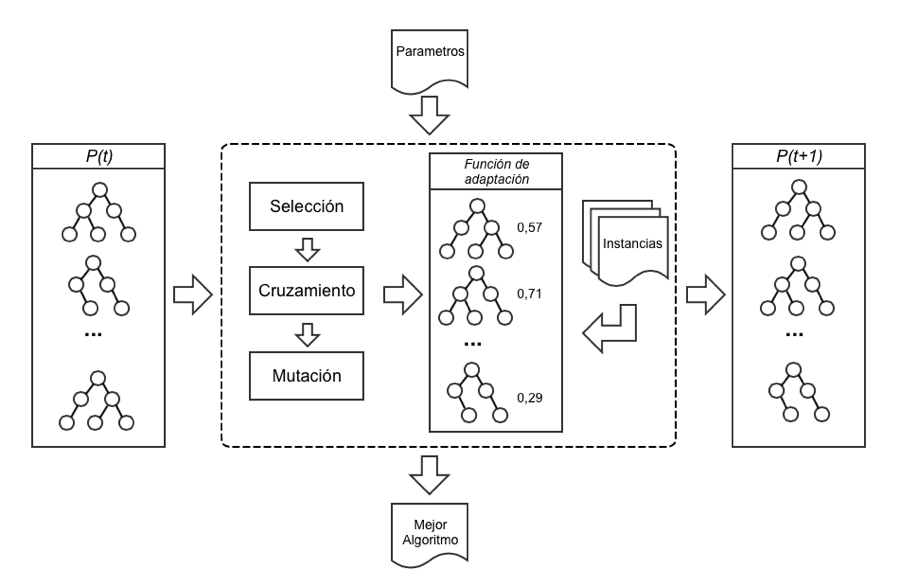
\includegraphics[width=14cm]{images/cap2/computacion_evol2.png}
    \captionof{figure}{Estructura general de la computación evolutiva \citep{contreras_2013}.}\label{fig:computacion_evol}
\endgroup

Los componentes principales para la CE son:
\paragraph{Representación} es una representación del problema a tratar en el mundo real, esto quiere decir que debe existir coherencia entre el espacio de solución a recorrer y el problema en si, para posteriormente poder interpretar la solución producida por la evolución.

\paragraph{Población} Son los individuos que se encuentran en una generación. Se les llama individuos a posibles candidatos que pueden dar solución al problema que se quiere resolver. La población compone la unidad de evolución, donde los individuos se mantienen estáticos, mientas que la población va cambiando.

\paragraph{Inicialización} El objetivo es generar la población inicial, la cual puede ser de forma aleatoria o utilizando alguna heurística. Generalmente,se utiliza la generación aleatória, ya que es la propia CE la que se encargará de mejorar a los individuos.

\paragraph{Función de mejora o {\it fitness}} Es la encargada de medir la aptitud de un individuo de la población (poli et. al 2008). Esta función permite discriminar quienes son los individuos que pasarán a las siguientes generaciones y quiénes no. Es así, dependiendo del problema, la evolución toma una tendencia de maximizar o minimizar, y va guía a generar buenas soluciones.

\paragraph{Operadores de variación} Los operadores permiten generar nuevos individuos a la población a partir de los ya existentes. Su objetivo principal es recorrer nuevas y mejores soluciones no producidas en las generaciones anteriores, con el fin de resolver el problema planteado de la mejor forma.

Los operadores clasicos se destacan tres: cruzamiento, mutación y selección (Falkenauer,1998).
\paragraph{El cruzamiento} Es una operación binaria que permite el intercambio de material entre dos individuos, teniendo como resultados, dos nuevos individuos con información híbrida en cada uno.

\paragraph{La mutación} Opera sobre un individuo, y se aplica para generar diversidad de población.

\paragraph{La selección} Se encarga de obtener la cantidad de los mejores individuos que sobrevivirán al proceso.

\paragraph{Criterio de parada}: Los criterios de parada se pueden diferenciar en dos casos. El primero es conocer el valor óptimo de la solución y que éste sea alcanzado. El segundo puede ser que se han acabado los recursos tales como el máximo tiempo de CPU, un periodo de tiempo, no hay variación en la población, etc. Dentro de la computación evolutiva, existen diversos métodos que utilizan este concepto de una forma más específica de acuerdo a su representación. En el artículo \citep{kouchakpour_2009} se presenta una de las clasificaciones, que se pueden realizar de las variantes de CE. Ésta puede ser vista en la Figura \ref{fig:metodosCE}.

\begingroup
    \centering
    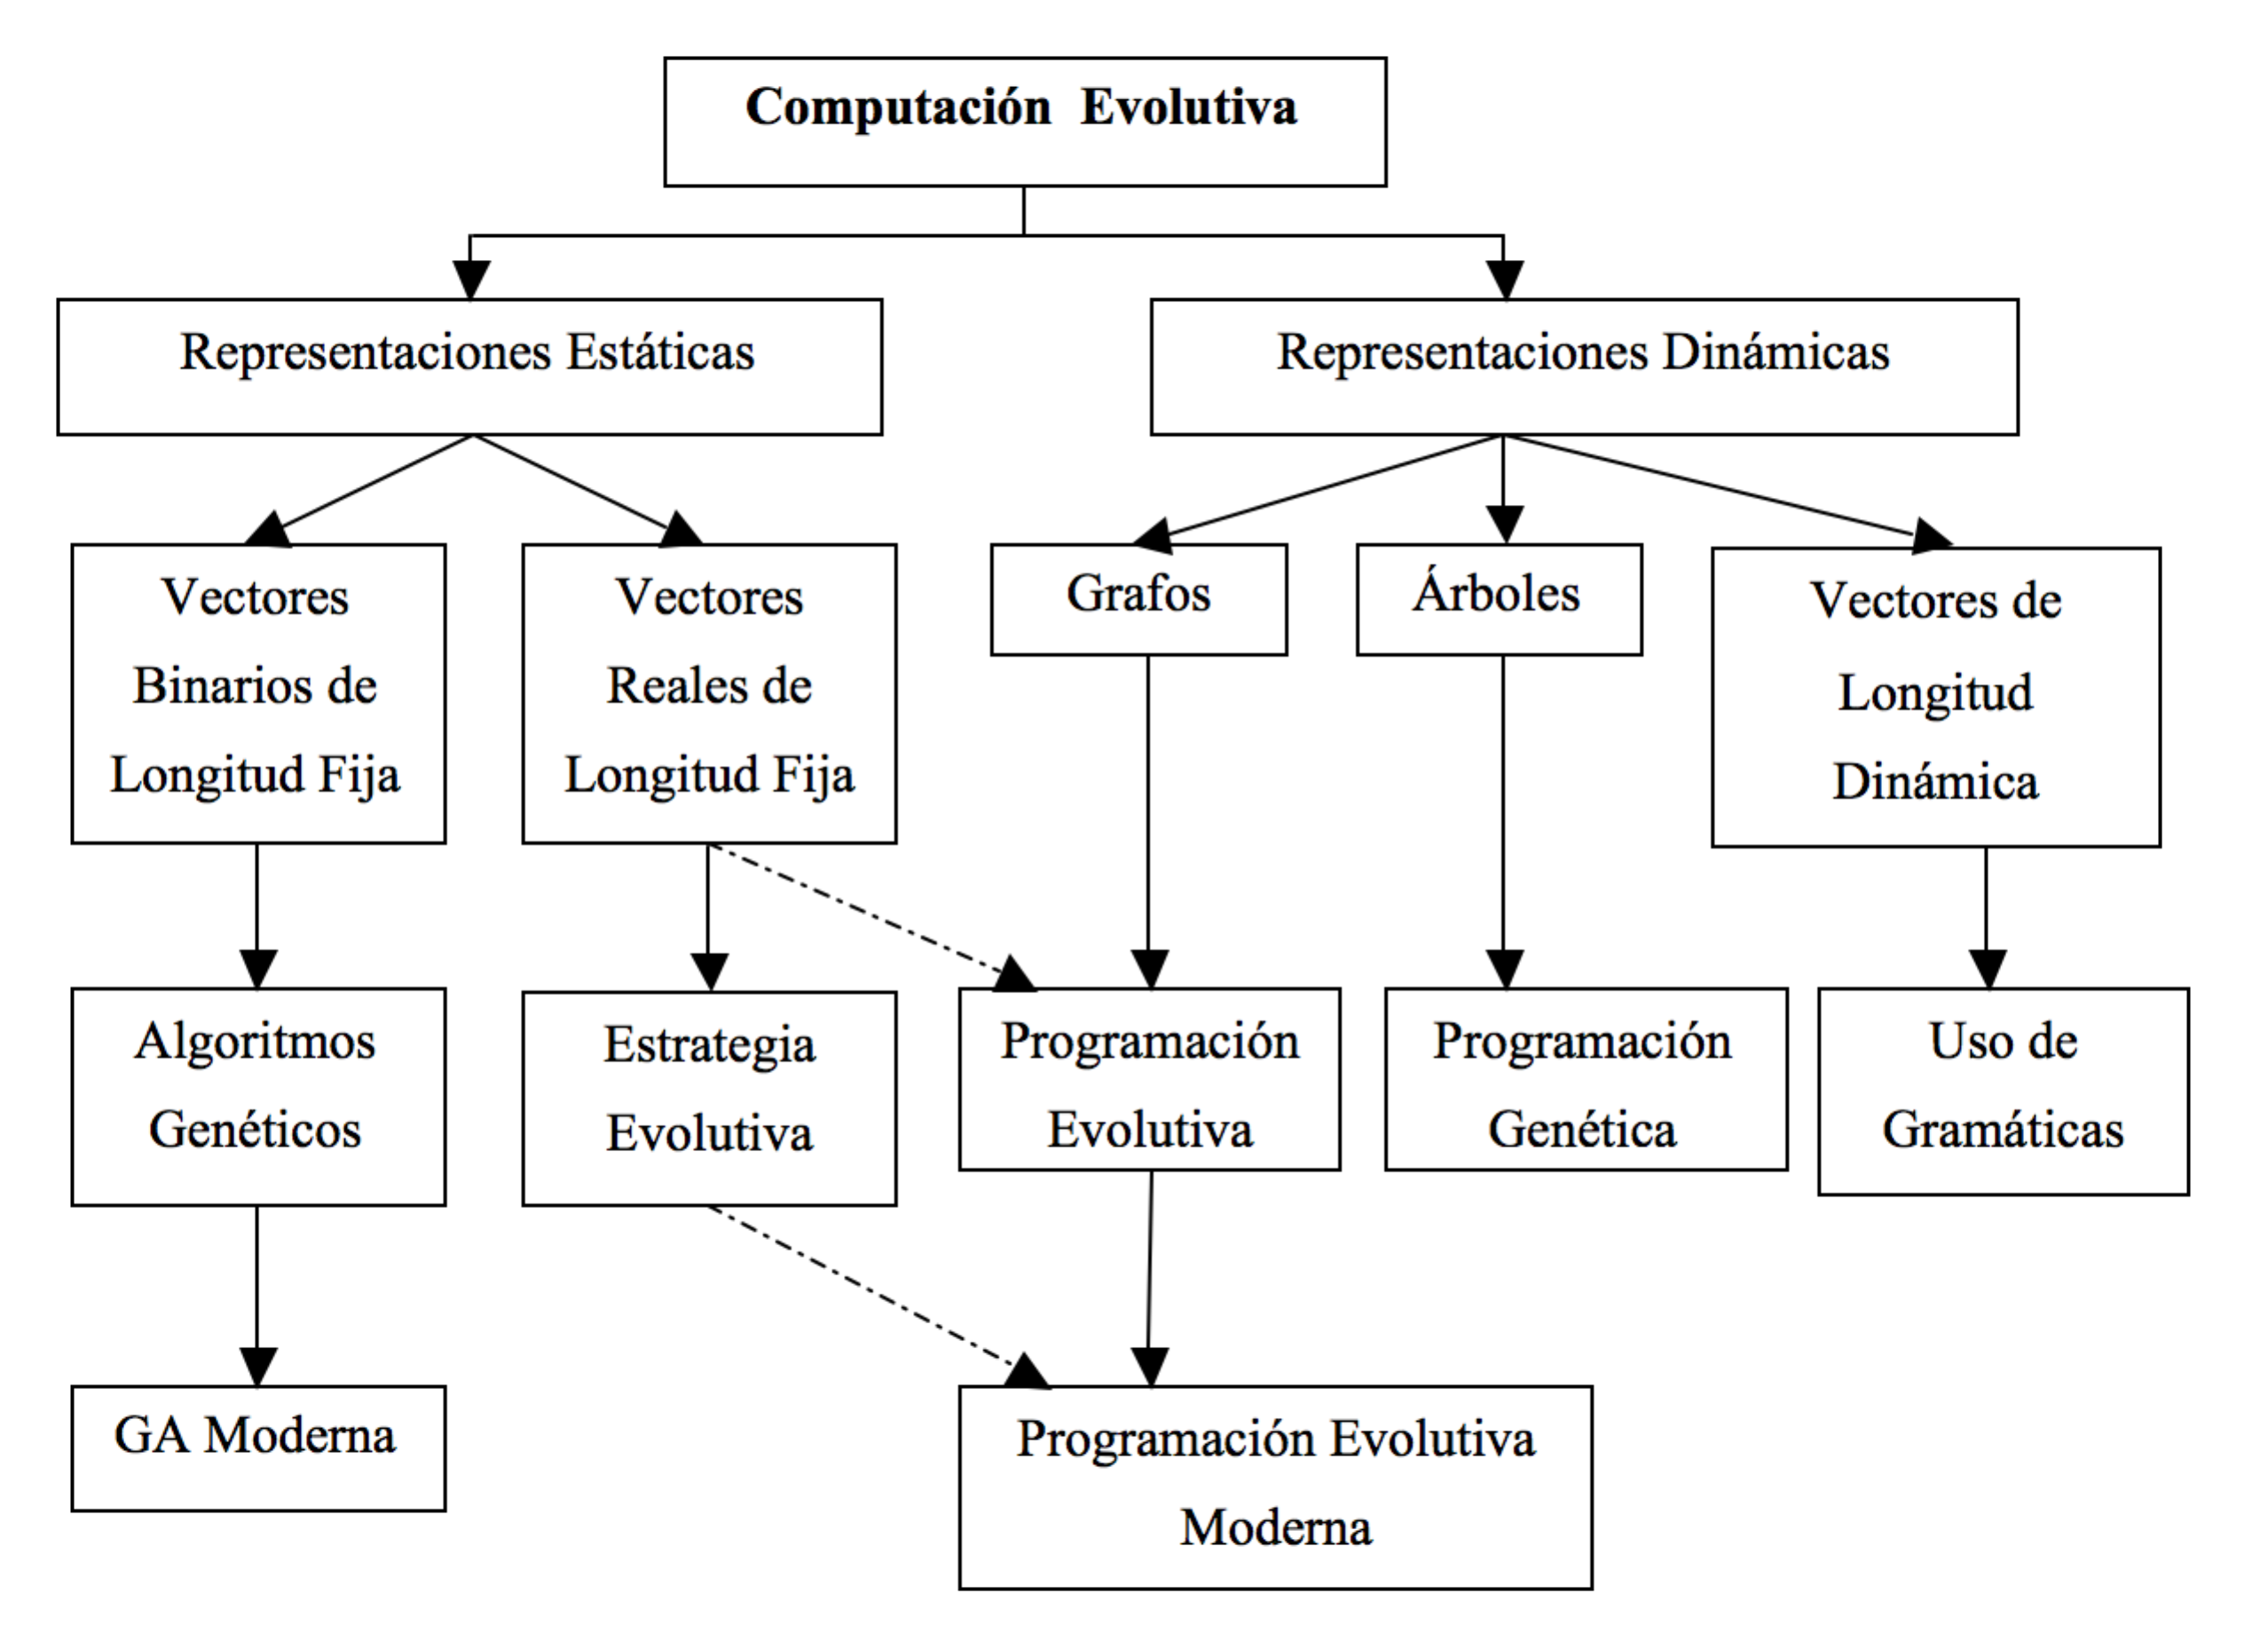
\includegraphics[width=14cm]{images/cap2/metodosCE.png}
    \captionof{figure}{Métodos de la CE basados en el tipo de representación \citep{kouchakpour_2009}.}\label{fig:metodosCE}
\endgroup

\subsection{Programación Genética}
\label{cap:pg}


Una de las tareas más desafiantes de la ciencia de la computación, consiste en que un computador pueda dar solución a problemas sin la necesidad de ser programados de manera explícita. \cite{samuel1959some} declaró:

\textit{¿Cómo pueden los computadores aprender a resolver un problema, sin ser programados explícitamente para ello? En otras palabras, ¿Cómo pueden los computadores hacer lo que tiene que hacer, sin explicitar exactamente cómo tiene que ser hacerlo?}

La Programación Genética (PG) es una técnica de Computación Evolutiva que mediante la generación de código computacional, es capaz de resolver problemas automáticamente, sin la necesidad de que un usuario especifique o conozca la estructura de la solución \citep{poli_2008}. A pesar de no poder garantizar los resultados por ser esencialmente un proceso evolutivo, ha sido muy exitosa y se han encontrado formas inesperadas de resolver problemas \citep{holland_1975}.

En la PG, el proceso evolutivo comienza con una población inicial generada aleatoriamente, la cual es representada por programas computacionales, donde cada individuo es ejecutado y evaluado en virtud de su medida de adaptación frente a un conjunto de casos de prueba propios del problema. Esto se puede apreciar en la figura XX que presenta el diagrama de flujo de los pasos básicos de la PG.


La PG posee tres operadores genéticos, basándose en la selección natural de Darwin, la superviviencia del más apto (operador de selección),la reproducción (operador de cruzamiento) y la mutación. Los operadores se utilizan para crear las nuevas generaciones de individuos que reemplazarán las anteriores \citep{poli_2008}. Generalmente la solución inicial tiene una muy mala calidad, pero algunos individuos serán más aptos que otros. Estas diferencias de adaptación que presenta cada individuo son explotadas a través de las generaciones, y lentamente aquellas caracteristicas individuales que ayudan a resolver el problema, se harán mas comunes en la población. Este funcionamiento se puede ver apreciado en el Algoritmo \ref{alg:programacion_genetica}
\begin{algorithm}[H]
    \begin{algorithmic}[1]
        \STATE {\em Generar Población Inicial aleatoria}
        \WHILE {\em La condición de término sea verdadera}
            \STATE {\em Ejecutar cada programa y determinar su \textit{fitness}}
            \STATE {\em Seleccionar uno o dos individuos-programas de la población para participar en las operaciones genéticas.}
            \STATE {\em Crear nuevo programa mediante la aplicación de las operaciones genéticas}
        \ENDWHILE
    \end{algorithmic}
    \caption{Programación genética}\label{alg:programacion_genetica}
\end{algorithm}



%LISTOOOOOOOOOOOOOOOOOOOOOOO

Para resolver un problema utilizando la PG, \cite{koza_1992} define cinco pasos, los cuales se detallan a continuación:

\begin{itemize}
	\item \textit{Definición del conjunto de terminales}: Permite identificar el conjunto de terminales que van a ser utilizados por los individuos en la población. Los terminales pueden consistir en constantes que representen entradas, sensores o variables de estado, funciones sin argumento, entre otros.

	\item \textit{Definición del conjunto de funciones}: Permite identificar el conjunto de funciones, las cuales corresponden a operaciones elementales posibles, de las que se sospecha puedan intervenir en el cómputo de alguna solución, tales como operaciones aritméticas ($+$,$-$,$*$,$/$), funciones matemáticas ($seno$,$coseno$,$logaritmo$), operaciones booleanas ($and$,$or$,$not$), operaciones condicionales ($if$-$then$-$else$) y funciones que causan iteraciones ($while$,$for$).

	\item \textit{Definición de la medida de aptitud}: Es la encargada de medir la aptitud de los individuos de la población para resolver un problema. La medida de aptitud varía según el problema al que se quiere dar solución. Generalmente se utiliza el error relativo.

	\item \textit{Parámetros de control}: Consiste en escoger los valores de ciertos parámetros que permiten calibrar la evolución. Estos valores pueden ser la probabilidad de cruzamiento, mutación, tipo de selección, entre otros.

	\item \textit{Especificar el criterio de designación de resultado y término de ejecución}: Se puede designar al mejor individuo de todo el proceso de la evolución, a los $k$ mejores individuos de las últimas generaciones u otra alternativa que sea apropiada al problema que se quiere resolver. Para el criterio de término, se puede fijar un número máximo de generaciones o algún equivalente de éxito como un valor de evaluación de desempeño, entre otros.
\end{itemize}



Adicionalmente, para una correcta implementacion de la PG, existen dos propiedades que se deben considerar al momento de construir las funciones y terminales:

\begin{itemize}


\item \textit{Suficiencia}: Las funciones y terminales utilizados deben ser suficientes para representar una solución para el problema \citep{koza_1992}. Si el diseño no es apropiado o suficientemente representativo, la PG no podrá encontrar una solución factible al problema planteado.

\item \textit{Clausura}: Cada función debe ser capaz de manejar de forma adecuada los argumentos que pueda recibir como entrada, estos son los posibles valores retornados por otras función definida en el conjunto y cualquier valor o tipo de dato que sea alcanzable desde el conjunto de terminales \citep{koza_1992}. La clausura no es una propiedad indispensable, en los casos que no se puede garantizar, se debe utilizar alternativas tales como, la eliminación de individuos o la penalización sobre su medida de aptitud cada vez que algún individuo contenga alguna construcción infactible.


% LISTOOOOOOOOOOOOOOOOOOOOOOOOOOOOOOOOOOO

%como entrada, ya sea que provengan de otras funciones definidas o parámetros que pueden alcanzar los terminales definidos.

%	\item Suficiencia del conjunto de funciones y terminales: la propiedad de suficiencia está relacionada con la capacidad de expresar un programa computacional que resuelva un problema planteado en términos de las funciones y terminales definidos para ello \citep{koza_1992}. Cada problema requiere un diseño apropiado, basado en un amplio conocimiento del dominio. En ocasiones, su definición puede llegar a ser muy difícil o virtualmente imposible \citep{koza_1992, poli_2006}.

%	\item Clausura del conjunto de funciones: la clausura es una propiedad deseable para el conjunto de funciones, pero no indispensable, ésta consiste en que cada función debe aceptar como argumentos el resultado . Existen casos donde no es posible garantizar la clausura del conjunto de funciones, en estas situaciones se debe utilizar alternativas tales como, la eliminación de individuos o la penalización sobre su medida de aptitud cada vez que alguno de ellos incorpore en su código alguna construcción infactible.

\end{itemize}


A partir de la última década del siglo $XX$, la PG ha sido considerada como un método "humano competitivo" para la resolución de problemas. Las principales razones de esta clasificación se debe a que la mayoría de los problemas planteados en inteligencia artificial, aprendizaje automático y sistemas adaptativos pueden ser formulados como una búsqueda de programas computacionales, y la técnica de PG entrega una forma satisfactoria de guiar la búsqueda en el espacio de programas computacionales \citep{affenzeller_2001}.

Turing, en el año 1948, advirtió correctamente que una posible aproximación a la inteligencia artificial incluiría un proceso evolutivo, donde un programa computacional (material hereditario) sea sometido a una modificación progresiva (mutación) bajo la dirección de la selección natural \citep{koza_poli_2005}.

Un resultado generado por un método automatizado puede ser clasificado como “humano competitivo”, independiente del hecho de que sea generado de forma automática. Sin embargo, un resultado humanamente competitivo obtenido debe tener un cierto grado de complejidad, es por esto que un resultado generado por un método automatizado que resuelve un \textit{“toy problem”} (por ejemplo, las torres de Hanoi, apilamiento de bloques, caníbales y misioneros), no sería considerado como “humano competitivo”, debido a que la solución no es publicable como un nuevo resultado científico, sólo es de interés porque fue creado de forma automática.

Así, según Koza \citep{koza_2003}, una solución generada automáticamente para un problema es humanamente competitiva si ésta satisface uno o más de los ocho criterios que se muestran en la Tabla \ref{tab:human_comp}.

\begin{table}[ht]
\caption{Criterios para un resultado “humano-competitivo” \citep{koza_2003}.}\label{tab:human_comp}
\small
\centering
\rowcolors{2}{white}{blue!25}
\begin{tabular}{cl}
\hline
{\textbf{Nº}} & \multicolumn{1}{c}{\textbf{Criterio}} \\ \hline

A  & \begin{tabular}[c]{@{}l@{}} El resultado fue patentado como un invento, es una mejora de una invención patentada, \\o podría calificar como una nueva 		invención patentable.   \end{tabular}  \\
B  & \begin{tabular}[c]{@{}l@{}} El resultado es igual o mejor que un resultado científico aceptado y publicado en una \\ revista científica. \end{tabular}  \\
C  & \begin{tabular}[c]{@{}l@{}} El resultado es igual o mejor que un resultado que fue colocado en una base de datos o \\ archivo de resultados y gestionada por un panel internacional de expertos científicos reconocidos. \end{tabular}  \\
D  & \begin{tabular}[c]{@{}l@{}} El resultado es publicable como un nuevo resultado científico, independiente del hecho \\ que fue creado mecánicamente. \end{tabular}  \\
E  & \begin{tabular}[c]{@{}l@{}} El resultado es igual o mejor que un resultado reciente de un problema que ha tenido \\ sucesivos resultados cada
	vez mejores.  \end{tabular}                  \\
F  & \begin{tabular}[c]{@{}l@{}} El resultado es igual o mejor que un resultado que se consideró un logro en su campo \\ en el momento en que fue descubierto.	\end{tabular}                  \\
G  & \begin{tabular}[c]{@{}l@{}} El resultado soluciona un problema de dificultad indiscutible en su campo.	\end{tabular}                  \\
H  & \begin{tabular}[c]{@{}l@{}} El resultado está entre los mejores o gana una competencia regulada que incluye \\ participantes humanos.	\end{tabular}  \\
\hline
\end{tabular}
%\caption*{(Elaboración propia, 2015)}
\end{table}

La obtención de resultados humanamente competitivos ha incentivado el crecimiento del campo de la computación genética y evolutiva, esto se debe a que la obtención de estos resultados depende del progreso, desarrollo y perfeccionamiento de los métodos de búsqueda genéticos y evolutivos. No obstante, a medida que resultados humanamente competitivos sean generados, irán apareciendo problemas más desafiantes.

\section{Revisión de la literatura}
\label{cap:rev_literatura}

\subsection{Generación automática de algoritmos}
La generación automática de algoritmos (GAA) ha sido utilizada los últimos años para resolver distintos problemas de optimización combinatoria. En este proceso, los algoritmos pueden ser generados mediante el uso de hiper-heurísticas que poseen estructuras que permiten ser interpretadas como algoritmos. Se pueden encontrar varios trabajos que utilizan la PG para realizar la GAA \citep{contreras_2013, drake_2014, parada_2015}.

El proceso para diseñar hiper-heurísticas que permitan obtener una solución a un problema de optimización combinatoria consta de tres fases \citep{alinia_2012}. La primera corresponde a la formulación matemática del problema. La segunda fase es el diseño de heurísticas de bajo nivel que permitan entregar una solución apróximada al problema. Y la tercera fase procesa, por medio de una hiper-heurística, diferentes combinaciones de las heurísticas definidas en la segunda fase. El proceso de selección de heurísticas se puede realizar a través de métodos de adaptación que buscan los mejores resultados en el espacio de soluciones de acuerdo con una medida de rendimiento \citep{parada_2015}.

%El desarrollo de la generación automática de algoritmos (GAA) es un tema que ha tomado mayor importancia en los últimos años. En este proceso, algoritmos pueden ser generador por hiper-heurísticas que poseen estructuras que pueden ser interpretadas como algoritmos. En la literatura existen varios trabajos que utilizan la PG para realizar la GAA \citep{contreras_2013, drake_2014, parada_2015}.

%El diseño de hiper-heurísticas para problemas de optimización combinatoria es un proceso que consta de tres etapas \citep{alinia_2012}. La primera de ellas es el problema a resolver, definido por su formulación matemática. La segunda consiste en heurísticas de bajo nivel que permiten dar solución al problema de forma aproximada. Finalmente, la tercera permite procesar por medio de una hiper-heurística diferentes combinaciones de las heurísticas definidas en la etapa 2. Por otra parte, la correcta selección de heurísticas es determinada en el presente trabajo, debido a que la selección de heurísticas o combinación de éstas es un problema de optimización combinatoria.

%El proceso de selección heurística se puede realizar a través de métodos de adaptación o meta-heurísticas que buscan los mejores resultados en el espacio de soluciones. El proceso de búsqueda encuentra una heurística que ofrece la mejor opción en cada movimiento de acuerdo con alguna medida de rendimiento \citep{parada_2015}.

\subsection{Heurísticas y meta-heurísticas}

En la actualidad, para resolver problemas computacionalmente complejos es necesario desarrollar algoritmos más avanzados. Los algoritmos exactos suelen requerir una gran cantidad de tiempo debido al tamaño del espacio de soluciones factibles. Para solucionar éste problema, han sido desarrollados los algoritmos aproximados, que, mediante el uso de heurísticas y meta-heurísticas, permiten encontrar soluciones que se acercan a una mejor solución. Los algoritmos heurísticos utilizan funciones especiales, las que están diseñadas para encontrar el espacio de soluciones de forma inteligente.


%Hoy en día los computadores son utilizados para resolver problemas computacionalmente complejos. Para resolver estos problemas es necesario desarrollar algoritmos más avanzados. Los algoritmos exactos para resolver estos problemas pueden requerir un tiempo inaceptable dado el espacio de búsqueda de soluciones factibles. Para hacer que un algoritmo de búsqueda obtenga soluciones en un tiempo aceptable, se han desarrollado algoritmos aproximados. Este tipo de algoritmo ocupa heurísticas y meta-heurísticas para encontrar las soluciones. Los algoritmos heurísticos utilizan las funciones especiales, diseñadas para averiguar el espacio solución de forma inteligente.

En la Figura \ref{fig:tax_opt} se muestra la clasificación de diferentes problemas de optimización, los cuales están divididos en dos categorías: algoritmos exactos y algoritmos aproximados \citep{desale_2015}.

\begin{figure}[H]
%\begingroup
    \centering
    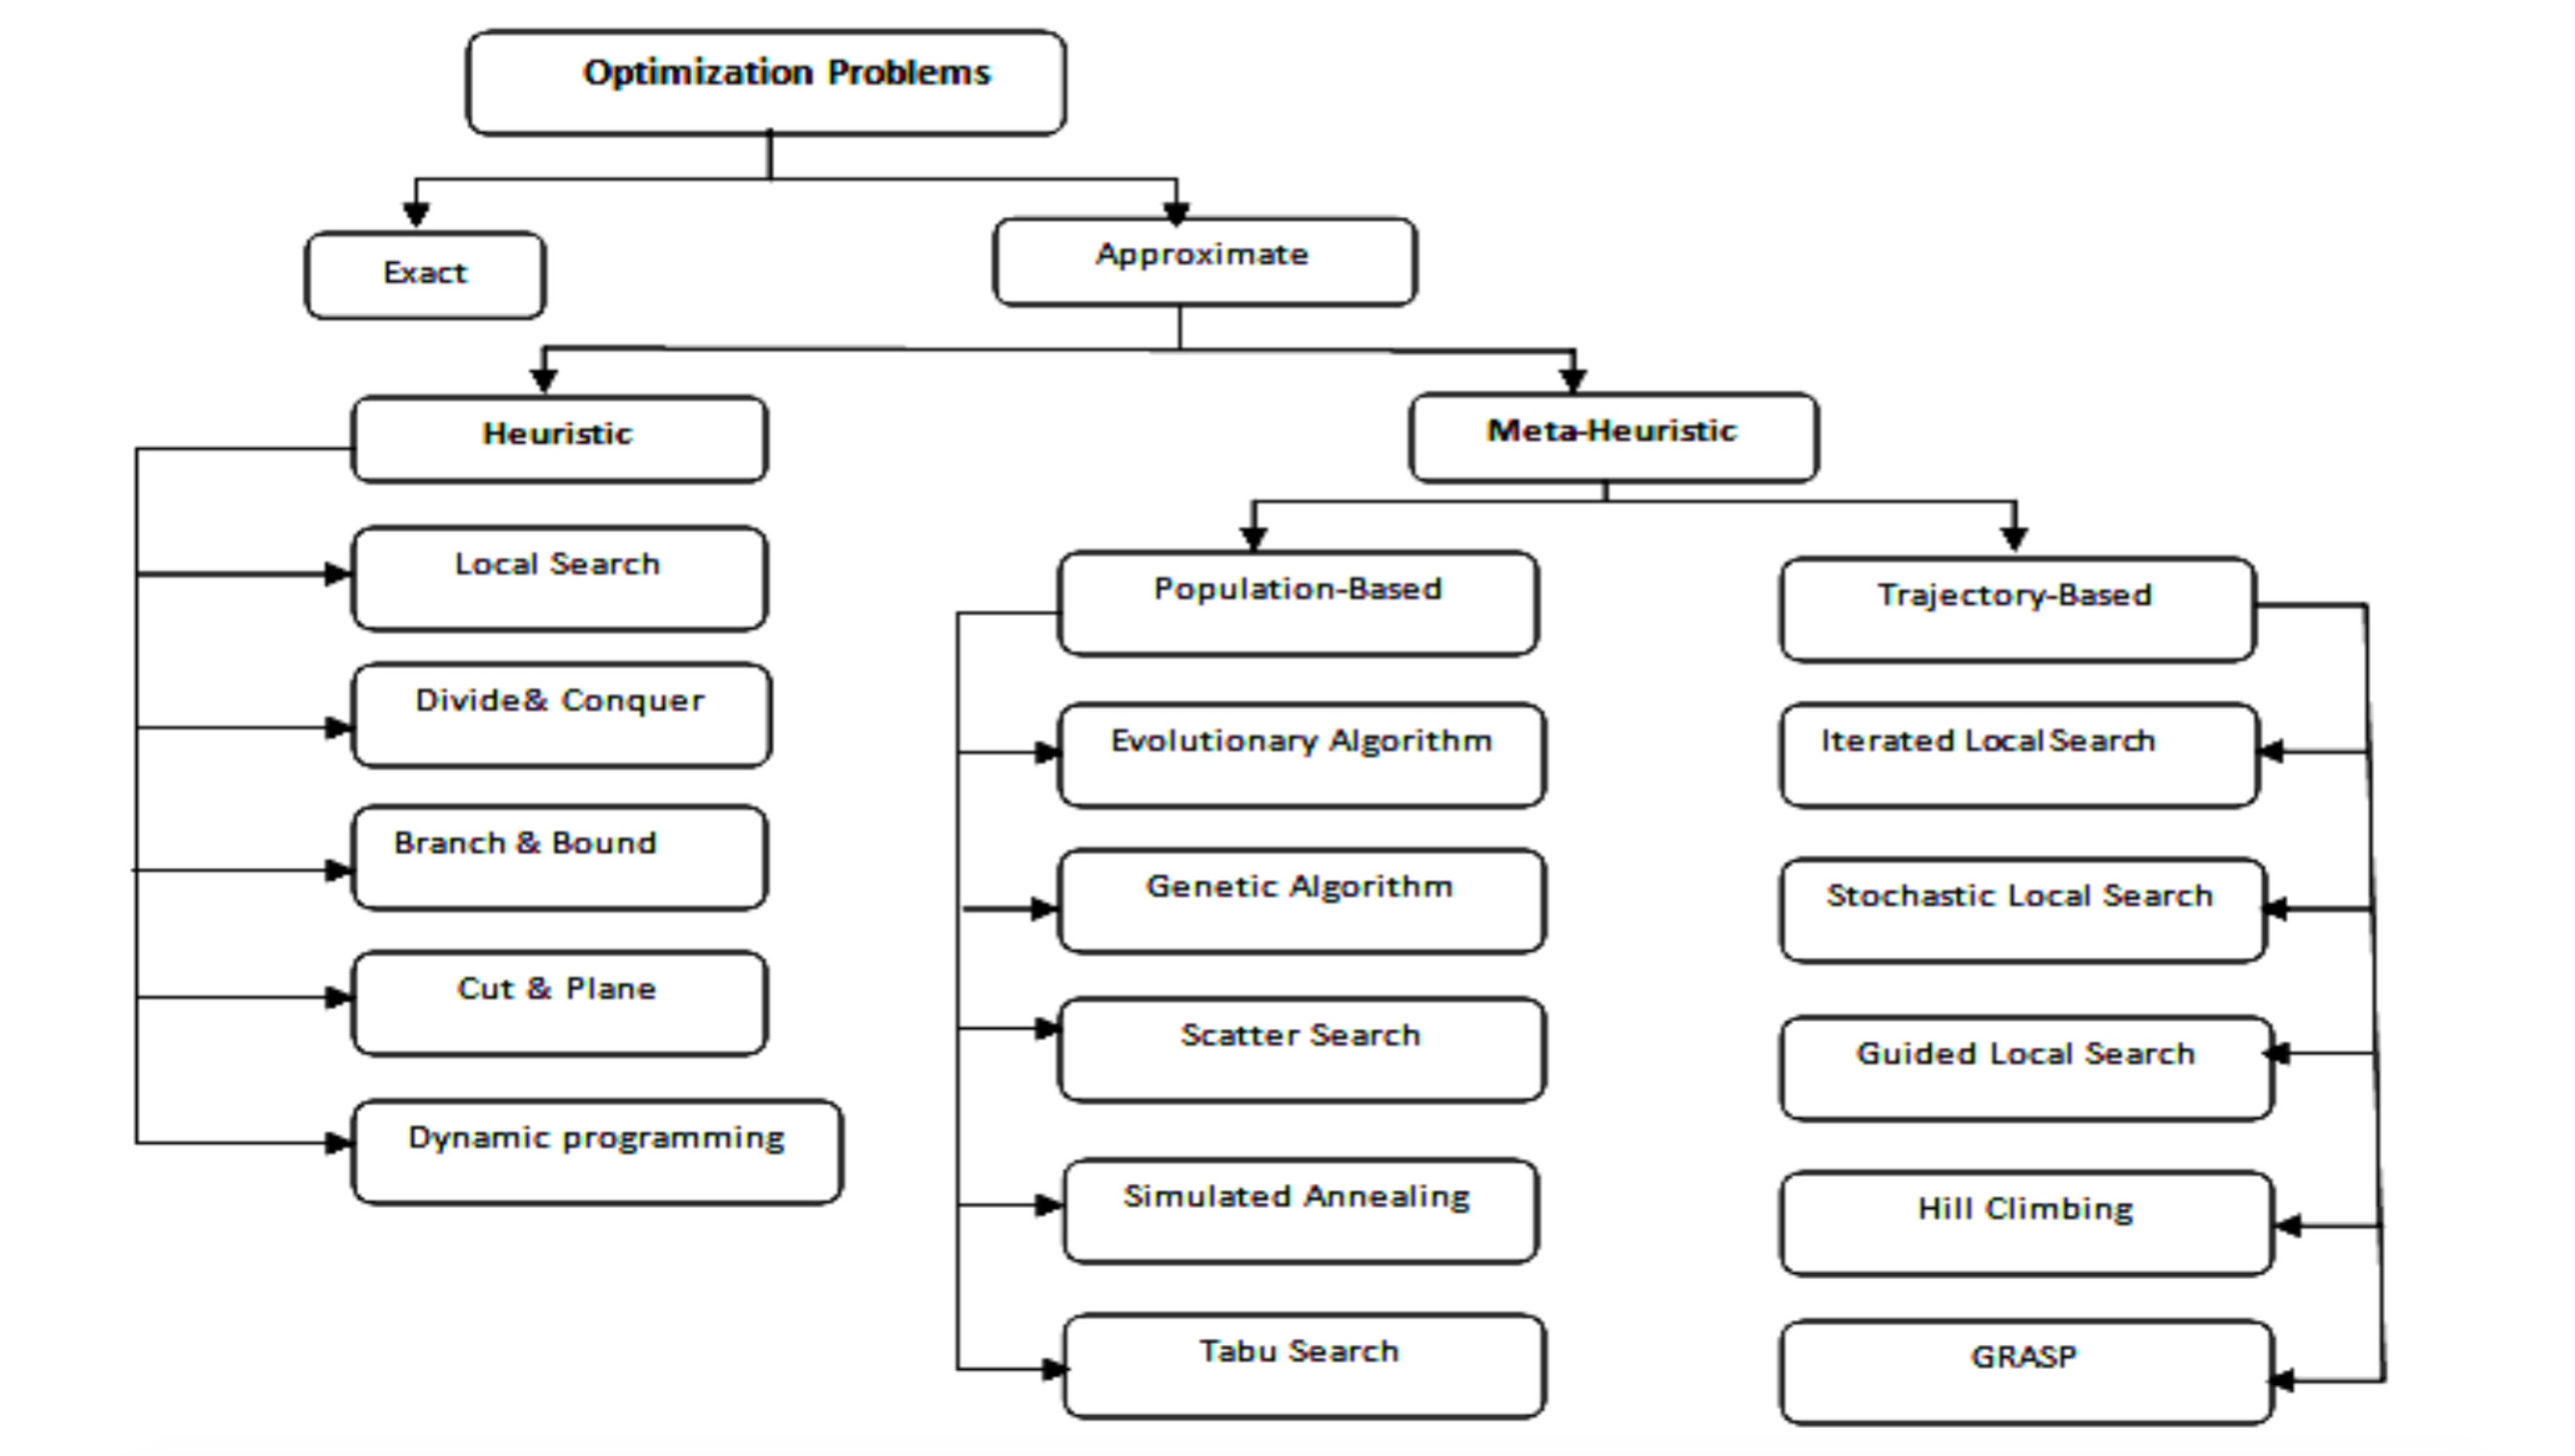
\includegraphics[width=16cm]{images/cap2/tax_opt.png}
    \captionof{figure}{Métodos utilizados para resolver problemas de optimización \citep{desale_2015}.}\label{fig:tax_opt}
%\endgroup
\end{figure}


Los algoritmos meta-heurísticos son el proceso de generación iterativo que guía una heurística para explorar y explotar el espacio de búsqueda.

Las heurísticas y meta-heurísticas son utilizadas para encontrar una solución óptima en un espacio de búsqueda discreto en problemas de optimización combinatoria. Un ejemplo es el problema del vendedor viajero, donde la búsqueda del espacio de soluciones factibles crece exponencialmente en función del tamaño del problema aumenta, lo que hace inviable la realización de una búsqueda exhaustiva de la solución óptima \citep{desale_2015}.

%Heurística y meta-heurísticas se utilizan para la optimización combinatoria en la que se busca una solución óptima en un espacio de búsqueda discreto. Un problema de ejemplo es el problema del vendedor viajero, donde la búsqueda del espacio de soluciones factibles crece exponencialmente a medida que el tamaño de los problemas aumenta, lo que hace inviable una búsqueda exhaustiva de la solución óptima \citep{desale_2015}.

\subsection{Hiper-heurísticas}

El término de hiper-heurística fue utilizado por primera vez en el año 2000 para lograr describir una heurística que escoge heurísticas en el contexto de la optimización combinatoria. Mientras que la automatización del diseño de heurísticas se remonta a la década de 1960. La definición de hiper-heurísticas  se refiere a un método de búsqueda o mecanismo que permite seleccionar o construír la heurística que resuelve problemas de búsqueda de cálculo de aprendizaje. Se pueden diferenciar dos categorías: la selección de heurísticas y la generación de las mismas. La características de las hiper-heurísticas es que operan en un espacio de búsqueda de una heurística y no directamente en el espacio de búsqueda de soluciones del problema en cuestión \citep{burke_2013}.

El proceso para generar algoritmos en forma automática puede entenderse como una hiper-heurística, o como una metodología, cuando la generación automática de algoritmos se realiza mediante el uso de la programación genética y definición del proceso evolutivo. En ambos casos existen elementos comunes que permiten generar artefactos que resuelvan el problema en estudio, un proceso de mejora guiado por una función objetivo, entre otros. El proceso de generación de algoritmos busca obtener una estructura que se expresa mediante un árbol sintáctico y luego se decodifica para su posterior comprensión e interpretación. El objetivo del proceso es poder extraer conocimiento nuevo para recrear los algoritmos existentes en la literatura. Además, la GAA permite generar algoritmos que contemplen el uso de las mejores heurísticas o algoritmos existentes para el problema. Mientras que las hiper-heurísticas son utilizadas para resolver en forma eficiente el problema sin necesidad de realizar una interpretación del resultado obtenido \citep{burke_2013}.

%El término hiper-heurística es relativamente nuevo; fue utilizado por primera vez en el año 2000 para describir una heurística que escoge una heurística en el contexto de la optimización combinatoria. Sin embargo, la idea de automatizar el diseño de la heurística no es nueva; este se remonta a la década de 1960. La definición de hiper-heurística se ha ampliado recientemente para referirse a un método de búsqueda o mecanismo para seleccionar o generar la heurística para resolver problemas de búsqueda de cálculo de aprendizaje. Dos categorías principales de hiper-heurística pueden ser considerados: la selección de heurística y la generación de heurística. La característica distintiva de hiper-heurística es que operan en un espacio de búsqueda de una heurística (o componentes heurísticos) en lugar de hacerlo directamente en el espacio de búsqueda de soluciones para el problema que se está abordando \citep{burke_2013}.

%El proceso de generación automática de algoritmos puede ser visto como una metodología o como una hiper-heurística cuando la generación automática de algoritmos se realiza a través de la programación genética y siguiendo los pasos canónicos, que consiste en la generación de funciones y terminales, y definición del proceso evolutivo. Ambas tienen elementos en común que permiten generar dispositivos, aparatos o algoritmos que resuelvan el problema en estudio, un proceso gradual de mejora guiado por una función objetivo, etc. La diferencia entre ambas es que un proceso de generación de algoritmos busca generar una estructura que se expresa mediante un árbol sintáctico y posteriormente se descodifica su correspondiente pseudo código para que sea perfectamente comprensible e interpretable por el ser humano. El objetivo de realizar la generación de esta forma es que el ser humano pueda extraer conocimiento nuevo para recrear los algoritmos existentes en la literatura. También la GAA permite generar algoritmos que contengan las mejores heurísticas o algoritmos disponibles para el problema que provienen de la literatura. A diferencia de ello, las hiper-heurísticas son ocupadas para resolver eficientemente el problema sin que sea necesario realizar una interpretación de la estructura o del código obtenidos. Asimismo, las hiper-heurísticas que se han experimentado hasta ahora utilizan distintas formas de obtener las estructuras de los problemas de optimización general \citep{burke_2013}.



\subsection{Instancias}
\label{cap:instancias}


-------------------------((PENDIENTE))------------------------

Durante los últimos años, se han desarrollado cada vez algoritmos más sofisticados para problemas de optimización. Estos algoritmos incluyen distintos métodos o técnicas, los que son sometidas a estudios experimentales que tienen por objetivo determinar que algoritmo obtiene un mejor rendimiento, usualmente éstos se basan en conjuntos de instancias públicas. El teorema de \textit{no free lunch} (NFL) dice que no existe un algoritmo que sea superior a todos los demás algoritmos en todas las instancias posibles de un problema. Si un algoritmo se declarase como mejor que otro conjunto de algoritmos, entonces es posible esperar que existan instancias que aún no han sido probadas. Es por esto que una de las claves para poder realizar un correcto estudio es caracterizar las instancias del problema de acuerdo a su dificultad y al espacio de soluciones que las representa \citep{smith_2012}.

Las características más sencillas de una instancia para un problema de optimización son las que se definen como parte de la sub-clase de la instancia: características como el número de variables y restricciones, o si las matrices que almacenan los parámetros son simétricas, etc.

Para el PVV, una forma de clasificar las instancias es mediante la distribución de costos que posee (distancias entre los nodos o ciudades), donde se muestra el número de valores distintos que poseen las distancias \citep{smith_2012}. Las instancias a utilizar para este problema, son obtenidas de la TSPLib \citep{reinelt_1991}. Esta librería contiene instancias ampliamente utilizadas en la literatura, las que en su totalidad cuentan con su valor óptimo y, en algunos casos, con una posible solución.

La clasificación para las instancias del PM-01 ha sido altamente estudiada por Pisinger. La clasificación más común es la realizada en base a la relación que poseen el beneficio y peso de cada uno de los ítems de una instancia, donde propone una variedad de grupos. Estos grupos poseen características desde una igualdad beneficio-peso hasta grupos donde no existe relación alguna entre éstos. Adicionalmente, es propuesta una clasificación con relación a las magnitudes de los valores que pueden alcanzar los elementos \citep{pisinger_2005}. Las instancias a utilizar para este problema son las utilizadas por Pisinger \citep{pisinger_2005}.

\subsection{Revisión de la literatura para PCMR}



El PCMR, que pertenece a la clase NP-Hard \citep{joksch1966shortest}, consiste en encontrar un camino o cadena de aristas $P_{cad}$ desde un vértice inicial $v_s$ perteneciente a \emph{V}, a un vértice final $v_e$ también perteneciente a \emph{V}, que minimice el costo total de aristas en $P_{cad}$ y que además la suma de los recursos o pesos de cada aristas no exceda un máximo de recurso a consumir denotado \emph{W} \citep{dumitrescu2001algorithms}. Su formulación matemática es la siguiente:
%Sea \emph{G =(V,A)}, un grafo sin ciclos y dirigido, donde \emph{V=\{1,2...n\}}  es un conjunto de vértices, $|V|=n$ y \emph{A} es un conjunto de arcos tal que $A= \{(i,j):i,j \in V, i \neq j\}$. Cada arco \emph{(i,j)} perteneciente a \emph{A} posee un costo no negativos $C_{i,j}$ y posee además un recurso o peso no negativos $W_{i,j}$.

%Teniendo en cuenta estas definiciones, el problema CSP se puede formular como un problema de programación entera binaria de la siguiente manera:

\begin{equation}
min \sum_{i,j \in A}^{}{c_{ij}x_{ij}}
\end{equation}

\begin{equation}
sujeto  \sum_{j:(i,j) \in A }^{}{x_{ij}} - \sum_{k:(k,i) \in A}^{}{x_{ki}} = \begin{cases}
      1              & \mbox{si } i= v_s   \\
      0 			 & \mbox{si } i= 2,..... n-1 \\
      -1 			 & \mbox{si } i= v_e
   \end{cases}
\end{equation}

\begin{equation}
\sum_{i,j: (i,j) \in A}^{}{w_{ij}x_{ij}} \leq W
\end{equation}

\begin{equation}
x_{ij} /x_{ij} \in  \left \{0,1 \right \} , (i,j)  \in A
\end{equation}

%La variable $x_{ij}$ son variables binarias que se encuentran asociadas a cada arco $(i,j)$. Si el arco está incluido en la ruta óptima, entonces $x_{ij}=1$, en caso contrario $x_{ij}=0$. El parámetro $W$ representa el valor máximo del peso a no sobrepasar para la suma de los pesos de las aristas $w_{ij}$, y $c_{ij}$ es el costo asociado. De ésta forma,
%La ecuación (2.1) se plantea el problema de minimización, donde se suman todos los costos considerados en el camino,
La ecuación (2.2) da a conocer que debe ser una cadena conexa desde el nodo inicial $v_s$ a $v_e$, y la ecuación (2.3) plantea que la suma de los pesos de las aristas consideradas en el camino no debe sobrepasar el peso $W$ \citep{santos2007improved}.


%El problema del camino mínimo con restricción (PCMR), que pertenece a la clase NP-Hard \citep{joksch1966shortest}, consiste en encontrar la ruta más corta entre dos puntos, pero no debe sobrepasar un peso $W$ también asociado al camino. Existen diversas aplicaciones prácticas en el mundo real para el CSP, como el problema de ruteo de buses \citep{cho2007intermodal}, gestión de aeronaves \citep{zabarankin2002optimal}, usos militares \citep{royset2009routing}, entre otros. La formulación matemática es la siguiente:


%\begin{eqnarray}
%\min \sum_{i, j \in A}^{m} c_{ij}x_{ij}
%\end{eqnarray}
%Sujeto a
%\begin{eqnarray}
%\sum_{j : (i, j) \in A}^{m} x_{ij} - \sum_{k : (k, i) \in A}^{m} x_{ki}
%&=&
%\left\{
%\begin{array}{rrl}
%  1   & si  & i = s\\
%  0   & si  & i = 2, \ldots, m - 1\\
%  -1  & si  & i = t
%\end{array}
%\right.\\
%\sum_{i, j: (i, j) \in A}^{m} w_{ij}x_{ij} &\leq& W\label{form:2_3}\\
%x_{ij} \in \{0, 1\}&&  (i, j) \in A
%\end{eqnarray}
%La ecuación \ref{form:2_1} verifica que sea un camino conexo desde el nodo inicial $s$ al nodo final $t$. Mientras que la ecuación \ref{form:2_2} da a conocer el dominio de $x_{ij}$. La ecuación \ref{form:2_3} plantea que la suma de los pesos de las aristas consideradas en el camino no debe sobrepasar el peso $W$.

Las estrategias utilizadas para el PCMR se pueden clasificar en dos categorías principales, programación dinámica y relajación lagrangiana. Los métodos basados en la programación dinámica también se conocen como \textit{label setting} o \textit{label correcting}. Una de las características de este tipo de algoritmos es que en instancias de tamaño razonable, pueden ser muy veloces; sin embargo, para redes que pueden tomar dimensiones muy grandes podrían dejar de ser una buena alternativa, esto debido a que el número de etiquetas que deben ser almacenadas  puede ser muy grandes y como consecuencia pueden ser imposibles de manejar.

Uno de los primeros algoritmos pertenecientes a esta categoría fue propuesto por \cite{joksch1966shortest}, el cual fue extendido por \cite{dumitrescu2003improved}, comparandse con tres algoritmos \cite{dumitrescu2001algorithms,hassin1992approximation,lorenz2001simple} a los que supera en término de tiempo computacional y requisitos de memoria. Los autores afirman también que la integración entre las técnicas de relajación langrageana y pre-procesamiento podrían mejorar el tiempo de ejecución.

Posteriormente, se presentan un enfoque de etapas para abordar el camino mínimo con un conjunto de restricciones o recursos (PCMG) \cite{zhu2012three}. Para ello se propone un algoritmo pseudopolinomial llamado TSA en tres etapas: la primera es un pre-procesamiento de las instancias reduciendo los arcos y los vértices, disminuyendo el espacio de búsqueda, el segundo es un proceso de \textit{setup} para transformar el PCMG a un PCM, el tercero es un procesamiento iterativo de búsqueda. El TSA es comparado con CPLEX (REFERENCIA FALTANTE) y con el algoritmo \textit{label setting} \citep{dumitrescu2003improved} para cuatro tipos distintos de problemas, mostrando abordar de forma eficaz los casos de prueba, pero el tiempo de ejecición aumenta a medida que los problemas se van haciendo más grandes en cantidad de nodos y conjunto de recursos.

El segundo enfoque para dar solución al PCMR se basa en el uso de la relajación lagrangiana para resolver la formulación de programación entera del problema. La eficiencia de este enfoque se basa en la eficacia de los algoritmos de ruta más corta sin restricciones subyacentes. Un algoritmo exacto para el problema PCMR basado en relajación Langragiana al cual es denotado como LRA (lagrangian relaxation algorithm)\citep{santos2007improved}. El LRA se compara con métodos de \textit{k-shortest path} y con métodos de relajación langragiana, ambos introducidos por \cite{handler1980dual}. Los resultados de estas pruebas indican que el LRA puede abordar grandes problemas teniendo ventajas sobre los otros métodos en términos de tiempo computacional y en el uso de memoria. Sin embargo, los autores comparan su algoritmo sólo con \cite{handler1980dual}, y no con los algoritmos mejorados de \citep{dumitrescu2003improved}.

Luego, se expone un nuevo algoritmo basado en relajaciones Langragianas con enumeraciones de caminos mínimos al cual denominan LRE (\textit{lagrangian relaxation and enumeration}), el cual se sostiene en técnicas de pre-procesamientos \citep{carlyle2008lagrangian}. En el trabajo se utiliza cuatro grupos de casos de prueba y se compara con el \textit{label setting} \citep{dumitrescu2003improved}, donde el LRE resuelve hasta el doble de casos que el \textit{label setting} en un tiempo de 30 minutos. Sin embargo, existen casos que el LRE no supera al \textit{label setting}, debido a la existencia de grandes distancias entre las cotas inferiores y superiores, teniendo un tiempo de ejecución más prolongado. Mientras que en el 2009, se da a conocer un enfoque Langragiano dual al cual se denomina eliminación agresiva de costos (AEE) \citep{muhandiramge2009simultaneous}. Consiste en una versión modificada del algoritmo expuesto por \citep{carlyle2008lagrangian}. AEE se compone de dos etapas principales: primero relaja el problema con métodos duales Langragianos con iteraciones, todo ello mediante la restricción de pesos con pasos de pre-procesamiento, después, aborda el problema basándose en las cotas de la red ya reducida por el pre-procesamiento. Se da a conocer que se podrían mejorar los resultados siempre y cuando se encuentren buenos parámetros iniciales, como las cotas iniciales o múltiplos iniciales, lo cual no se investigó en el artículo científico.

Posteriormente, se propone un método exacto llamado \textit{Pulse} que maneja redes de gran escala para el problema del PCMR \citep{lozano2013exact}, encontrando mejores resultados en los 180 casos propuestos en la literatura, respecto al algoritmo de \cite{santos2007improved}, logrando aceleraciones de hasta 60 veces. También supera favorablemente al algoritmo propuesto por \cite{dumitrescu2003improved}, logrando aceleraciones de hasta 900 veces con las dos series de casos propuestos para el problema.

En uno de los últimos trabajos se propone un modelo mejorado llamado Ameba para abordar el problema del PCMR \citep{zhang2013adaptive}. El modelo Ameba consiste en un conjunto de tubos interconectados que emulan a esta bacteria, y que posteriormente, construyen un modelo matemático \citep{nakagaki2001path}. Para resolver el problema, adaptan el modelo de Ameba al problema de PCMR y después integran un proceso de relajación Langragiana. Se afirma que el método es capaz de abordar problemas del PCMR, pero sólo con los casos de selección de rutas en redes de transporte y de computadora propuestos en su investigación.



\subsection{Revisión de la literatura para PACMG}
\label{cap:rev_lit_pvv}



El PACMG, que pertenece a la clase NP-Hard \citep{dror2000generalized}, consiste en un grafo no dirigido cuyos nodos son divididos en $k$ clúster, para determinar un árbol de cobertura de costo mínimo que incluya sólo un vértice de cada cluster. Se define matemáticamente por un grafo no dirigido $G = (V,E)$ de $n$ vértices, $m$ aristas y $ V_{1},..., V_{k}$ una división de $V$ en $k$  subconjuntos (clúster), donde, $ V_{1}~\cup~V_{2}~\cup ~V_{3}~....\cup ~V_{k}$ con $ V_{l}~ \cap ~V_{s} = \Phi~~ \forall j,s \in \left \{1,...,s\right \}~~ y~~ l \neq s$. Las aristas son definidas sólo entre vértices que pertenecen a clusters diferentes, el costo de una arista $e = (i,j) \in E$ está dado por $e_{ij}$. %La %Figura \ref{fig:sim}, presenta un ejemplo de GMSTP con 5 clusters y 17 vértices, se puede apreciar que para cada cluster, sólo se selecciona un nodo, y el costo de la función objetivo del GMSTP corresponde a sumar cada uno de los  asociados.

%El problema del árbol de cobertura mínima generalizado (PACMG), que pertenece a la clase NP-Hard \citep{dror2000generalized}, consiste en encontrar en un grafo no dirigido un árbol de cobertura de costo mínimo. Los vértices del grafo son divididos en \textit{clusters}, y el árbol de cobertura debe incluir sólo un vértice de cada conjunto. Sea $G=(V,A) $ un grafo no dirigido de n nodos, y $V_1, \hdots, V_m$ una división de $V$ en $m$ subconjuntos llamados clusters, es decir,$V = V_1 \cup V_2 \cup \hdots \cup V_m$  y $V_l \cap V_k = \emptyset, \forall l, k \in I = \{1, \hdots, m\}, l \neq k$. Denotamos $c_{ij} \in \mathbb{R} $ como el costo de una arista $e = (i,j) \in A$.

Su formulación matemática propuesta por \cite{pop2002generalized} es la siguiente:

Considerando,

$$ \min \sum_{i, j \in A}^{m} c_{ij}x_{ij} $$
\vfill

$$
x_e = x_{ij} =
\left\{
\begin{array}{cl}
	1	& \mbox {Sí la arista } e = (i, j) \in E \mbox{ es incluye en la solución}\\
	0	& \mbox{ en otro caso}
\end{array}
\right.
$$

$$
z_i =
\left\{
\begin{array}{cl}
	1	& \mbox {Sí el nodo } i \mbox{ es incluye en la solución}\\
	0	& \mbox{en otro caso}
\end{array}
\right.
$$

$$
w_{ij} =
\left\{
\begin{array}{cl}
	1	& \mbox {Sí el arco } (i, j) \in A \mbox{ es incluido en la solución}\\
	0	& \mbox{en otro caso}
\end{array}
\right.
$$
\vfill

Se utilizan las notaciones vectoriales $ x = (x_{ij})$, $z = (z_i)$, $w = (W_{ij})$ y la notación $x(E') = \sum_{\{i, j\} \in E'} x_{ij}$, para $E' \subseteq E$, $z(V') = \sum_{i \in V'}z_i$, para $V' \subseteq V$ y $w(A') = \sum_{(i, j) \in A'} w_{ij}$, para $A' \subseteq A$
\vfill



\begin{eqnarray}
	\min	& \sum_{e \in E} c_e x_e&\\
	s.t.	& z(V_k) = 1			& \forall k \in K=\{1, \hdots, k\}\\
			& x(E(S)) \leq z(S - i)	& \forall i \in S \subset V, 2 \leq |S| \leq n - 1\\
			& x(E) = k - 1			& \\
			& x_e \in \{0, 1\}		& \forall e \in E\\
			& z_i \in \{0, 1\}		& \forall i \in V\
\end{eqnarray}



La ecuación (2,6) asegura que exactamente n vértice es seleccionado desde cada clúster, la ecuación (2,7) impide que existan ciclos, y la ecuación (2,8) asegura que existan \textit{k-1} aristas en la solución.


Este problema ha sido abordado con diversos enfoques. Uno de los enfoques en la programación entera, en los cuales se han utilizado distintas formulaciones tales como: \textit{formulations based on tree properties},\textit{ flow based formulations}, \textit{formulations based on arborescence properties} y \textit{based on Steiner tree properties} \citep{pop2009survey}. Sin embargo, no son capaces de resolver problemas de gran tamaño y a pesar de la variedad de formulaciones, sólo algunas estrategias encuentran buenas cotas inferiores, pero el tiempo de ejecución es demasiado \citep{ferreira2012grasp} o son capaces de encontrar cotas para instancias grandes, debido a los altos recursos de memoria requeridos.


Otros enfoques para resolver el PACMG son las heurísticas constructivas y de mejora. Las heurísticas constructivas proporcionan la solución paso a paso, de manera tal, que se van añadiendo aristas a la solución hasta construir un PACMG. Típicamente, se utilizan adaptaciones de los conocidos algoritmos polinomiales de \textit{Prim}, de \textit{Kruskal} y de \textit{Sollin} \citep{papadimitriou1982combinatorial}. Las heurísticas de mejora comienzan con una solución inicial que se modifica iterativamente con el objetivo de encontrar mejores soluciones. Las primeras cuatro heurísticas propuestas para dar solución al problema (dos de mejora y dos constructivas), fueron propuestas por \cite{dror2000generalized}, siendo la más efectiva, una de las constructivas.

Otro de los enfoques utilizados para abordar el problema es la combinación de diferentes técnicas, heurísticas y metaheurísticas. Uno de los enfoques es el de \textit{greedy} llamado PROGRES, que es un algoritmo \textit{greedy} aleatorio que incorpora tres técnicas de diversificación: aleatoriedad, perturbación y penalización \citep{haouari2006upper}, obteniendo un 92,5\% de resultados óptimos, de los casos de prueba que son generados al azar con un máximo de 1000 vértices y 1000 aristas.

Posteriormente, se proponen cinco heurísticas \citep{ferreira2012grasp}, mostrando un buen desempeño tanto en instancias de pocos vértices como en instancias de gran tamaño, en la calidad de solución y en el tiempo computacional. Además, proponen mejoras que combinan el procesamiento con una búsqueda local, mejorando las soluciones considerablemente, pero aumentando el tiempo de cómputo. Luego, se proponen seis versiones de GRASP \citep{talbi2009metaheuristics} que consisten en la combinación de los métodos anteriores y la técnica de \textit{path-relinking}, lo cual aumenta el rendimiento para las seis heurísticas de GRASP, permitiendo mejorar aún más las soluciones, pero también incrementando el tiempo de cómputo.

Uno de los últimos trabajos propone combinaciones heurísticas produciendo nuevos algoritmos para el PACMG de forma automática, utilizando parte de las técnicas ya existentes en la literatura \citep{contreras2016multi}. Los algoritmos son construidos utilizando componentes heurísticos elementales, obteniendo desde los métodos descritos en la literatura, más las estructuras de control que dan forma al algoritmo, mediante el uso de la computación evolutiva, obteniendo algoritmos competitivos, en términos de la calidad de la solución obtenida con las heurísticas existentes para abordar el problema, donde se obtiene que el error promedio obtenido por el algoritmo, de los 251 casos de prueba utilizados, es más bajo que el eror promedio de las heurísticas propuestas por \cite{golden2005heuristic} y \cite{ferreira2012grasp}.


\subsection{Revisión de la literatura para PVVG}
\label{cap:rev_lit_pvv}

El problema PVVG, que pertenece a la clase NP-Hard \citep{srivastava1969generalized,henrylab1969record}, consiste en encontrar un recorrido en el que existen \textit{clusters} o grupos predefinidos y el viajero debe visitar exactamente un nodo en cada \textit{cluster} minimizando el costo total del viaje. La formulación matemática es el siguiente:
%Sea $G = (V,A)$ un grafo donde $V = {1, 2,…, n}$ corresponde al set de nodos, mientras que  $A = { (i, j): i, j \in V, i \neq j }$ corresponde al conjunto de arcos direccionales o caminos, mientras que $c_ij$ indica el costo de recorrer cada uno de los arcos desde el nodo $i$ hasta el nodo $j$. Además $V_1, V_2,…, V_k$ sean subconjuntos de $V$ que no se superponen y que representan cada uno de los conjuntos del problema. La formulación matemática del SPP es el siguiente:



% \begin{figure}[H]
%   \center
%    \includegraphics[scale=.8]{img/TSP.png}
%   \label{fig:TDA}
% \end{figure}
\begin{eqnarray}
\sum_{i = 1}^{m} \sum_{j = 1}^{m}c_{ij}x_{ij}
\end{eqnarray}
Sujeto a
\begin{eqnarray}
\sum_{i = 1}^{m} \sum_{j = 1}^{m}c_{ij}x_{ij} &=& 1\\
\sum_{j = 1}^{m} \sum_{i = 1}^{m}c_{ij}x_{ij} &=& 1\\
\sum_{j = 1}^{m}x_{ji} - \sum_{j = 1}x_{ij}   &=& 0\\
&x_{ij} \in \{0, 1\}&
\end{eqnarray}


Las ecuaciones (2.12) y (2.13) garantizan que cada uno de los vértices es visitada exactamente una vez
, y la ecuación (2.14) asegura que no existan ciclos.


El PVVG es un problema al cual se le ha dedicado bastantes trabajos. Diversos investigadores  \citep{noon1993efficient,laporte1999computational,lien1993transformation,ben2003transformations} han propuesto transformar el problema en una instancia del problema del vendedor viajer (PVV). En una primera mirada, el concepto de transformar un problema que no ha sido tan trabajado a otro muy conocido, da la impresión de que se podrían obtener resultados prometedores. Sin embargo, al tratarse de una conversión, se debe lidear con aspectos técnicos que afectan los resultados. Uno de ellos, se requiere una solución exacta de la instancia PVV, debido a que una aproximación al óptimo puede representar una solución infactible para el PVVG (por ejemplo, qu la solución del PVV imprique recorrer más de un nodo por conjunto en el PVVG). Por otro lado, la estructura de las instancias del PVVG suelen ser distintas a las e los sistemas capaces de entregar una solución a instancias del PVV.

Una aproximación más eficiente para dar solución exacta al PVVG, es el algoritmo de ramificación y corte \citep{fischetti1995symmetric}. Utilizando este algoritmo, se ha logrado obtener soluciones a varias instancias, con un tamaño de hasta 89 grupos. Sin embargo, resolver instancias de mayor tamaño de forma óptima, es todavía una tarea muy complicada de realizar, aun con el poder de computo actual.


Posteriormente, se propone una heurística sofisticada llamada $GI^{3}$ (Generalización de inicialización, Inserción y Mejora) \citep{renaud1998efficient}. $GI^{3}$ es una generalización de la heurística $I^{3}$ presentado por \cite{renaud1996fast}. Esta heurística se compone de tres fases: la inicialización, en el que se construye una solución parcial, la inserción de un nodo de clústeres no visitado a la ruta hasta que se haya completado, y una fase que mejora la solución. El autor se compara con la heurística propuesta por \cite{fischetti1997branch}, en la que de 36 casos utilizados $GI^{3}$ entrega una mejor solución en 20 de los 36 casos, utilizando un tiempo computacional en promedio de 83,9 segundos.

Los algoritmos evolutivos también son utilizados para resolver al PVVG, uno de ellos es un algoritmo aleatorio de clave genética (RKGA) hibridado con una búsqueda local \citep{snyder2006random}. Se utiliza codificación de clave aleatoria para representar las soluciones. La ventaja de este esquema de codificación es mantener la viabilidad de las soluciones durante cruce y mutación. En un conjunto de 41 problemas de prueba estándar con distancias simétricas y hasta 442 nodos, la heurística encuentra soluciones que son óptimas en la mayoría de los casos y está dentro del 1\% del óptimo en gran parte de los problemas, exceptuando los de mayor dimensión, con tiempos de ejecución de 10 segundos en promedio.

Posteriormente, se propone un algoritmo memético, un nuevo procedimiento de cruce que se basa en \textit{large neighborhood search} \citep{bontoux2010memetic}. Con el objetivo de mejorar el rendimiento, se hibrididan el algoritmo con procedimientos de búsqueda local, es decir \textit{2-opt, 3-opt, de Lin-Kernighan} y mover procedimientos. Los resultados muestran que es un algoritmo con buen rendimiento, donde los 41 casos de prueba se abordan de manera óptima y en 37 de esos casos, la solución óptima se encuentra en cada ejecución del algoritmo propuesto.

Uno de los últimos trabajos es un algoritmo evolutivo inspirado por la competencia imperialista, llamado algoritmo competitiva imperialista (ICA). ICA tiene mejor rendimiento que los algoritmos genéticos y optimización por enjambre de partículas, el cual es mejorado empleando un nuevo esquema de codificación, un nuevo método de cruce y el nuevo mecanismo de mejora de los planes de desarrollo llamado imperialistas, el cual permite que el algoritmo sea más eficaz para explorar todo el espacio de soluciones \citep{ardalan2015novel}. ICA obtiene mejores rsultados en promedio en 27 casos de 53 superando el algoritmo de \cite{snyder2006random}. En otras obras, el ICA se aplica al problema de localización cubo por \cite{mohammadi2014sustainable}, el suministro de diseño de la red de la cadena por \cite{devika2014designing}, el problema de flujo de potencia con funciones de costos no lisos por \cite{ghasemi2014novel}, entre otros.

%\subsection{Sobre la investigación}
%\label{cap:sobre_inv}

%El objetivo del presente trabajo es evaluar la calidad de los algoritmos generados mediante los métodos de PG tradicional en comparación a los obtenidos utilizando la PG con co-evolución. Como se presentó a lo largo del capítulo 2, es posible apreciar que existe gran variedad de técnicas en la literatura para utilizar el paradigma de co-evolución. De acuerdo a los resultados presentados por los autores y la relación que estas técnicas poseen con la PG tradicional, se seleccionan los métodos propuestos por Chandra \citep{chandra_2014}, además del método propuesto por Arcuri y Yao \citep{arcuri_2014}. Estos métodos utilizan el concepto de poblaciones como islas o entornos evolutivos independientes donde las poblaciones comparten individuos cada un tiempo determinado y funciones de evaluación distintas, respectivamente. Ambos conceptos son interesantes de estudiar y poseen la particularidad de no ser excluyentes, por lo que el método propuesto incluye la unión de ambos métodos presentes en la literatura.

%Para la realización del método conjunto de PG con co-evolución utilizando islas, se consideran los dos entornos independientes y dos funciones de evaluación que también sean distintas entre sí. Estos cuatro elementos son combinados hasta obtener cuatro islas distintas que comprenden la combinación lineal de los elementos mencionados. Las islas comparten individuos en un tiempo determinado, y durante el resto del tiempo proceden a realizar el proceso evolutivo de la PG tradicional.

%Adicionalmente, es posible apreciar que existen factores a tener en cuenta para el desarrollo de la PG, principalmente que este trabajo se enfoca en dos problemas de optimización distintos. Por lo que en la metodología de trabajo se incluye la consideración de los diversos factores, tanto los propios de la PG, como los relacionados a cada uno de los problemas. Estos factores son analizados en los resultados del trabajo.

%Esto conduce a las siguientes preguntas de investigación que rigen el desarrollo de este trabajo, las que son descritas para cada uno de los problemas a abordar:

%La calidad de los algoritmos obtenidos para el problema del vendedor viajero simétrico mediante el esquema co-evolutivo, que considera la población completa dividida en cuatro islas, simulando ambientes distintos mediante un conjunto de instancias de evolución distintas y funciones de evaluación distintas, es mejor que los algoritmos obtenidos mediante un proceso evolutivo de una única población, con las mismas instancias de prueba y con una función objetivo que integra las funciones parciales del algoritmo con esquema co-evolutivo.

%La calidad de los algoritmos obtenidos para el problema de la mochila binaria mediante el esquema co-evolutivo, que considera la población completa dividida en cuatro islas, simulando ambientes distintos mediante un conjunto de instancias de evolución distintas y funciones de evaluación distintas, es mejor que los algoritmos obtenidos mediante un proceso evolutivo de una única población, con las mismas instancias de prueba y con una función objetivo que integra las funciones parciales del algoritmo con esquema co-evolutivo.

\chapter{Diseño de la experimentación}\label{cap:disegno_experimento}

La experimentación se lleva a cabo ejecutando los 3 problemas explicados en los capítulos anteriores, considerando tres etapas distintas. La tabla \ref{tab:diseno_experimental} presenta de manera esquemática el diseño experimental completo. La primera columna de la tabla representa cada uno de los problemas y la primera fila corresponde a las distintas etapas de la experimentación realizada. En la segunda columna se encuentran los algoritmos redescubiertos, basados en sus componentes elementales para los problemas básicos que se encuentran en la literatura mediante la PG. La tercera columna, que corresponde a la versión generalizada, presenta los algoritmos generados mediante la PG utilizando los componentes elementales que permitieron redescubrir los algoritmos de la primera columna. Finalmente, la cuarta columna corresponde a algoritmos que son encontrados mediante la PG, considerando los componentes elementales y de mejora o constructivos que permiten refinar los resultados.

\begin{table}[H]
	\centering
	\caption{Resumen del diseño experimental.}
	\begin{tabular}{llll}
				& Etapa I		& Etapa II						& Etapa III\\\hline
		PCMR	& $A_{11}(g_1)$	& $A_{12}(g_1, g_2, g_3)$		& $A_{13}(g_1, g_2, g_3)$\\
		PACMG	& $A_{21}(g_1)$	& $A_{22}(g_1, g_2, g_3, g_4)$	& $A_{23}(g_1, g_2, g_3, g_4)$\\
		PVVG	&				& $A_{32}(g_1, g_2)$			& $A_{33}(g_1, g_2)$\\\hline
	\end{tabular}
	\label{tab:diseno_experimental}
\end{table}

La estrategia seguida para obtener los algoritmos que se presentan en la tabla \ref{tab:diseno_experimental}, considera la incorporación gradual de nuevos terminales que permiten encontrar mejores resultados computacionales para cada uno de los problemas estudiados. En el caso de los algoritmos de la \textit{Etapa I}, se utilizan los componentes elementales del algoritmo de Prim y Dijkstra, además de componentes adicionales que permiten dar diversidad a la evolución los cuales son utilizados como terminales en la GAA. Los algoritmos de la \textit{Etapa II} utilizan los mismos terminales que en el caso de la \textit{Etapa I}, pero adaptados a las características propias de cada problema en particular. Para los algoritmos de la \textit{Etapa III}, son utilizados los mismos terminales de la \textit{Etapa II}, además de terminales de mejora que  permiten refinar los resultados obtenidos. Por ejemplo, el término $A_{23}(g1, g2, g3, g4)$ corresponde a un algoritmo que es encontrado para el problema 2 (PACMG) en el experimento 3 (versión generalizada con terminales de refinamiento), considerando los grupos de instancias $g1$, $g2$, $g3$ y $g4$.


%DESCOMENTAR ESTAS LÍNEAS SI EL CAPÍTULO TIENE FIGURAS O TABLAS
\addtocontents{lof}{{\bf \noindent Figuras del capítulo \arabic{chapter}}}
\addtocontents{lot}{{\bf \noindent Tablas del capítulo \arabic{chapter}}}

\section{Lógica del diseño}\label{cap:logica_diseno}

Para realizar la evaluación propuesta se desarrollan ocho experimentos generando algoritmos utilizando la PG, de los cuales dos corresponden a redescubrir los algoritmos polininomiales Dikjstra correspondientes al PCM  y Prim, que da solución al PACCM utilizando sus componentes elementales como terminales. Posteriormente tres experimentos que consisten en utilizar los componentes elementales del algoritmo Dijkstra para el PCMR y  Prim para el PACMG y PVVG. Finalmente, tres experimentos que utilicen componentes elementales de los algoritmos polinomiales, más algunas componentes de refinamiento que permiten mejorar los resultados. Los experimentos relacionados a la PG siguen la estructura utilizada por otros autores para la GAA \citep{contreras_2013, drake_2014,parada_2015}. Los experimentos son los siguientes:

\begin{itemize}
  \item \textbf{Experimento 1}: tiene por objetivo realizar la GAA utilizando la PG para redescubrir el algoritmo Dijkstra.
  \item \textbf{Experimento 2}: tiene por objetivo realizar la GAA utilizando la PG para redescubrir el algoritmo Prim.
  \item \textbf{Experimento 3}: tiene por objetivo realizar la GAA utilizando la PG implementando los componentes elementales del algoritmo de Dijkstra, los cuales se adaptan para el PCMR.
  \item \textbf{Experimento 4}: tiene por objetivo realizar la GAA utilizando la PG implementando componentes elementales del algoritmo de Prim, los cuales se adaptan para el PACMG.
  \item \textbf{Experimento 5}: tiene por objetivo realizar la GAA utilizando la PG implementando componentes elementales del algoritmo de Prim, los cuales se adaptan para el PVVG.
  \item \textbf{Experimento 6}: tiene por objetivo realizar la GAA utilizando la PG ocupando los mismos componentes que en el experimento 3 y componentes de mejora para el PCMR.
  \item \textbf{Experimento 7}: tiene por objetivo realizar la GAA utilizando la PG ocupando los mismos componentes que en el experimento 4 y componentes de mejora para el PACMG.
  \item \textbf{Experimento 8}: tiene por objetivo realizar la GAA utilizando la PG ocupando los mismos componentes que en el experimento 5 y componentes de mejora para el PVVG.

\end{itemize}

\section{Metodología del experimento}
\label{cap:experimento_tradicional}

Para el desarrollo de este experimento se utiliza la PG tradicional que fue descrita en la sección \ref{cap:pg}. Este experimento está dividido en dos etapas: proceso de evolución y el proceso de evaluación.

\subsection{El proceso evolutivo}

Se considera un proceso de aprendizaje para identificar la combinación adecuada de componentes que permitan resolver el problema. Para realizar el proceso evolutivo, son necesarios los siguientes pasos:

\begin{itemize}
  \item Definir una estructura de datos acorde al problema.
  \item Definir un conjunto de funciones y terminales que cumplan con las propiedades de suficiencia y clausura.
  \item Construir una función de evaluación acorde al problema para evaluar el rendimiento de los algoritmos generados.
  \item Seleccionar un conjunto de instancias del problema para adaptar los algoritmos a generar.
  \item Determinar los métodos de evolución y el valor de los parámetros de control del proceso evolutivo.
  \item Ejecutar el proceso evolutivo un número determinado de veces y recopilar estadísticas de los individuos generados.
  \item Seleccionar un conjunto de individuos para ser estudiados.
\end{itemize}

\subsection{El proceso de evaluación}

El proceso de evaluación mide el desempeño computacional que poseen los algoritmos generados en el proceso evolutivo. El desempeño de los algoritmos se determina a partir de que tan efectivos son para resolver el problema y cuánto tiempo tardan en hacerlo. Para esto se selecciona un conjunto de instancias distinto al grupo utilizado en la evolución. Los algoritmos son evaluados en este nuevo conjunto y para medir su calidad se utiliza el error relativo promedio(ERP), que consiste en el error relativo de los algoritmos obtenidos. Para cada grupo de instancias de evaluación $S$, se determina el porcentaje promedio por el cual el beneficio obtenido $z_{i}$ se encuentra distanciado de la mejor solución $o_{i}$ para cada instancia del conjunto $S$. Esto se representa en la ecuación \ref{eq:ERP_cap3}, donde $n_{s}$ representa el número de instancias del conjunto $S$.

\begin{equation}
  \label{eq:ERP_cap3}
  ERP_{s} =  \frac{1}{n_{s}} \cdot \sum\limits_{i=1}^{n_{s}} \frac{z_{i} - o_{i}}{z_{i}} \cdot 100\%
\end{equation}


\section{Consideraciones generales}
\label{cap:consideraciones}

Para trabajar con la PG en los ocho experimentos, se tienen en consideración algunos aspectos comunes tales como: el diseño, construcción, parametrización, calibración y \textit{testing} que se realizan previo a la ejecución de la PG. Esto debido a que es un proceso iterativo en cada experimento, y los efectos de un cambio en el diseño deben implementarse junto con realizar \textit{testing} para conocer sus efectos reales. 

Se realiza a continuación una descripción de las consideraciones.

\subsection{Resultados}

En los experimentos se busca encontrar algoritmos que solucionen los problemas planteados en la hipótesis, adicionalmente, estos resultados deben dar resultados similares o mejores a los obtenidos en trabajos previos.

\subsection{Instancias}

En los experimentos se utilizan instancias disponibles en la \textit{web} para uso investigativo y reconocidas por la comunidad científica asociada al área, las cuales difieren en cantidad para cada problema.
%La complejidad, división y cantidad a utilizar es especificada en el capítulo correspondiente al diseño del experimento de cada problema.

\subsection{Ejecuciones}

Aunque la PG utiliza generación aleatoria de números, es decir, una semilla distinta para cada ejecución, se observa que bastan tres ejecuciones para probar que los resultados son estadísticamente verdaderos. Según \cite{cantu_2003, li_2004} no es necesario realizar múltiples ejecuciones, ya que esto está sujeto a varios factores, como la variabilidad de las funciones, terminales, el problema en sí,  entre otros. Es por esto que se realizó un \textit{test} estadístico, utilizando la herramienta STATA (\textit{Data analysis and statistical software}) para comprobar si los datos se encuentran normalizados, para luego analizar si existe diferencia entre los resultados entregados por cada una de las ejecuciones realizadas. 
%En la Figura xx se puede ver los resultados de tres ejecuciones de la PG, donde el mejor individuo de cada una de ellas es evaluado en las 10 instancias con que se realizó la evolución. El \textit{test} de \textit{Shapiro-Wilk} da como resultado que los valores se encuentran normalizados o en algunos casos no existe observación (los resultados son iguales). Posteriormente, se realizó un \textit{test} de ANOVA que con 95\% de confiabilidad intenta probar si los valores poseen alguna diferencia significativa, resultando que no es posible determinar que exista esta diferencia.

%\begingroup
%    \centering
%    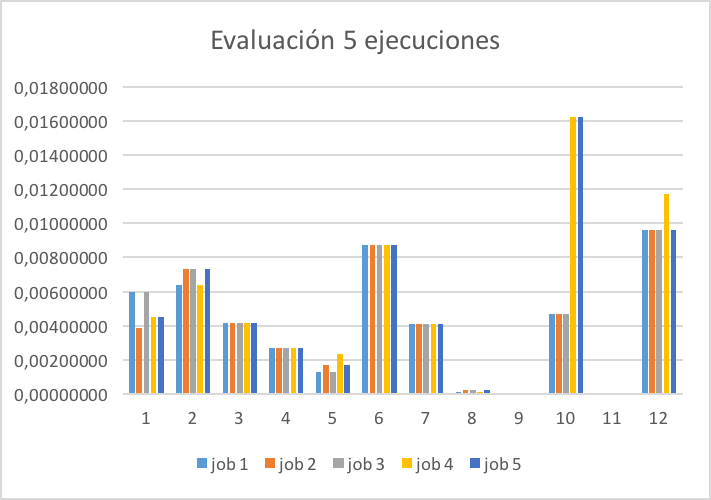
\includegraphics[width=14cm]{images/cap3/ejecuciones.png}
%    \captionof{figure}{Evaluación del mejor individuo sobre el conjunto de adaptación (Elaboración propia, 2015)}\label{fig:ejecuciones}
%\endgroup


\section{Estructuras de datos de los problemas}

Los algoritmos generados fueron construidos utilizando varias estructuras de datos. Las estructuras se diseñaron a partir de las caracteristicas de cada problemática y sus terminales y funciones. A continuación se dan a conocer los componentes de la estructura de datos para cada uno de los problemas:
 
%\paragraph{Algoritmo de Prim}
%\paragraph{Algoritmo de Dijkstra}

\paragraph{PCMR}

\begin{itemize}

\item \emph{Listas de Adyacencia de Grafo unidireccional (LAGU)}: Se guarda en esta lista de adyacencia, el grafo correspondiente a las instancias de evolución de los algoritmos. Este dato es estático, pues solo corresponde a información que deben leer los individuos y resolver durante la evolución.

\item \emph{Listas de incidencia de Grafo unidireccional (LIGU)}: Se guarda en esta lista de incidencia, el grafo correspondiente a las instancias que es usada en la evolución de los algoritmos, donde se busca almacenar las aristas que llegan a los nodos. Este dato es estático, pues solo corresponde a información que deben tomar los individuos y resolver durante la evolución.

\item \emph{Lista de etiquetas de solución (LES)}: Lista con las etiquetas del grafo. Se tiene una lista de etiquetas de tamaño $DIM_i$, siendo $i$ la instancia correspondiente de la etiqueta. Esta se inicializa con los valores de recursos y costo en infinito y con antecesor nulo.

\item \emph{Lista de nodos sin revisar (LNSR)}: Posee todos los nodos que no han sido etiquetados, vale decir, no se ha cambiado en la estructura \emph{LES}.

\item \emph{Último (U)}: Es el último nodo marcado que fue de menor costo y que, a partir de él, se siguen etiquetando nodos.

%\item \emph{Booleano de verificación de cambios } (HC): Toma el valor de verdadero cuando se realiza un cambio en \emph{LE} o en \emph{U}, y falso cuando no se ha hecho ningún cambio.
\end{itemize}

\paragraph{PACMG}

\begin{itemize}
\item Matriz de adyacencia (MAAC): En esta estructura se almacenan las distancias entre nodos, considerando la distancia euclidiana estipulado en las instancias. Las dimensiones de esta matriz son de $n x n$, dónde $n$ es la cantidad de nodos.

\item Mapa de relación cluster-nodo (MACN): Esta estructura almacena la relación existente entre el cluster y las características del nodo, además de almacenar por cada nodo, todos los posibles nodos con los que se puede conectar.

\item Listas de listas de la solución (LLS): En esta estructura se almacena el árbol de solución, donde cada posición i de la lista (raiz), contiene los nodos asociados $i$ (hijos).

\item Lista de Solución (LSAC): Almacena una lista de enteros, siendo estos, los nodos incluidos en la solución por cada cluster.

\end{itemize}	
	
\paragraph{PVVG}

\begin{itemize}
\item Matriz de adyacencia (MAVV): En esta estructura se almacenan las distancias entre nodos, considerando la distancia euclidiana estipulado en las instancias. Las dimensiones de esta matriz son de $N x N$, dónde $N$ es la cantidad de nodos (Referencia Parada Teoría de grafos).
  
\item Lista de nodos (LN): En esta estructura se almacenan estructura de nodos. Dicha estructura posee las características primordiales de un nodo: id, coordenadas y clúster al cual pertenece el nodo.  

\item Listas de adyacencia de clúster (LAC): Es una lista de listas. Cada posición i de la lista, contiene una lista de nodos asociados al clúster $i+1$ (Referencia Montgomery diseño y análisis).
 
\item Lista de nodos cercanos al centro (LNCC): Se construye una lista de nodos ordenados de menor a mayor según el centro de la instancia. El tamaño de esta estructura solo almacena $n/2$ nodos.
 
\item Lista de nodos cercanos al centro (LNLC):  Se construye una lista de nodos ordenados de menor a mayor según el centro de la instancia. El tamaño de esta estructura solo almacena $n/2$ nodos.

\item Lista de Solucion (LSVV): Almacena una lista de enteros, siendo estos, los nodos incluidos en la solución. El circuito se cierra conectado conectando el último de nodo de la lista con el primero de esta esta estructura. 
 
\end{itemize}	
	
\section{Identificación de Componentes Elementales}\label{cap:identificacion_componentes}

En esta sección se presenta el análisis para la obtención de los componentes elementales de los problemas fáciles.

\subsection{Descomponiendo Algoritmo Dijkstra}
El algoritmo de Dijkstra permite resolver de forma polinomial el PCM y en el algoritmo \ref{alg:alg41} se presenta su pseudocódigo.


\begin{algorithm}[H]
    \begin{algorithmic}[1]
        \STATE {\em Inicializar Etiquetas con antecesor nulo y costo INFINITO}
        \STATE {\em Inicializar una lista L con Todos los vétices del Grafo}
        \STATE {\em Etiquetar Vértice Inicial=[-,0]}
        \STATE {\em Marcar X = vértice Inicial}
        \STATE {\em Eliminar Vértice Incial de L}
        \WHILE {{\em Quedan Vértices en lista L}}
            \STATE {\em Actualizar etiquetas vecinos de X solo si el costo es menor.}
            \STATE {\em Buscar en L, el nodo con Etiqueta con costo más bajo (Nmin).}
            \STATE {\em Macar X=Nmin.}
            \STATE {\em Eliminar Nmin de L}
        \ENDWHILE
    \end{algorithmic}
    \caption{Algoritmo de Dijkstra}\label{alg:alg41}
\end{algorithm}

En el algoritmo \ref{alg:alg41}, de la línea 1 hasta la 5 se inicializan las estructuras de datos, mientras que en la línea 6 se puede observar el ciclo que permite realizar las iteraciones hasta encontrar el camino mínimo. La línea 7 es la encargada de actualizar las etiquetas de los vecinos del vértice seleccionado, la línea 8 busca en la lista de nodos disponibles el vértice seleccionado, la línea 9 es la encargada de marcar el vértice en la solución y la línea 10 es la que elimina el vértice marcado de la lista de vértices disponibles.

De esta forma el algoritmo se ejecuta hasta que todos los vértices hayan sido marcados. Esto se cumple con el criterio de término del ciclo \emph{while} del pseudocódigo, ya que a medida que se extraen los nodos de la lista \emph{L}, se van marcando y etiquetando los vértices del grafo.

Se puede observar que los componentes elementales del algoritmo están en la línea 6, que es la que permite que el ciclo siga hasta encontrar la solución, línea 7, encargada de actualizar las etiquetas y la línea 9  marcar el vértice en la solución. Generando así las siguientes funciones elementales:

\begin{itemize}


\item \textbf{Marca costo menor}: marca el vértice de costo menor en la solución.

\item \textbf{Etiquetar Dijkstra}: Actualiza las etiquetas del problema.

\item \textbf{Quedan vertices}: Verifica si ya se encontró el vértice final.
\end{itemize}

%Además se agregan funciones que permiten la diversidad en la evolución. Estas funciones son:


%\begin{itemize}

%\item \textbf{Etiquetador}: Cambia las etiquetas de los vecinos del último vértice marcado. Los vecinos deben ser vértices que no han sido marcados.


%\item \textbf{MarcaCostoMayor}: Elimina un vértice a la lista de vértices no marcados y es agregado como último vértice marcado. El vértice seleccionado es aquel que posea la etiqueta con mayor costo acumulado.

%\item \textbf{MarcarGradoMenor}: Elimina un vértice a la lista de vértices no marcados y es agregado como último vértice marcado. El vértice seleccionado es aquel que posea el menor grado.

%\item \textbf{MarcarGradoMayor}: Elimina un vértice a la lista de vértices no marcados y es agregado como último vértice marcado. El vértice seleccionado es aquel que posea el mayor grado.



%\item \textbf{EtiquetarVerificaPeso}: Cambia las etiquetas de los vecinos a partir del último vértice marcado verificando que el peso acumulado de la etiqueta no supere el peso máximo permitido. Si un vértice vecino ya fue etiquetado, se deja el que tenga menor costo acumulado. Si un vértice fue marcado anteriormente, no puede volver a ser etiquetado.

%\item \textbf{MarcarPonderado}: Elimina un vértice a la lista de vértices no marcados y es agregado como último vértice marcado. El vértice seleccionado es aquel que posea el menor valor que resulte de la multiplicación entre su peso acumulado y su costo acumulado.

%\item \textbf{MejorarDijkstra}: Cambia la etiqueta del último vértice marcado a partir de los vértice incidentes en él. Se realiza el cambio si el costo acumulado de la nueva etiqueta es menor al que va a reemplazar.

%\item \textbf{MejorarDijkstraPeso}: Cambia la etiqueta del último vértice marcado a partir de los vértice incidentes en él verificando que el peso acumulado de la etiqueta no supere el peso máximo permitido. Se realiza el cambio si el costo acumulado de la nueva etiqueta es menor al que va a reemplazar.

%\end{itemize}

%\item \textbf{MarcaPesoMenor}: Elimina un vértice a la lista de vértices no marcados y es agregado como último vértice marcado. El vértice seleccionado es aquel que posea la etiqueta con menor peso cumulado.

\subsection{Descomponiendo Algoritmo Prim}
El algoritmo de Prim permite resolver de forma polinomial el problema del aŕbol de cobertura de costo mínimo y en el algoritmo \ref{alg:alg42} se presenta su pseudocódigo.

%\subsection{Descomponiendo Algoritmo Prim}
\begin{algorithm}[H]
    \caption{Algoritmo de Prim}\label{alg:alg42}
    \begin{algorithmic}[1]
    	\STATE Inicializar una lista L con Todos los vétices del árbol
        \STATE Inicializar el árbol con un vértice arbitrario.
        \WHILE {\em Quedan Vértices sin utilizar}
        \STATE Añadir la arista de menor peso que se conecte con el árbol.
        \STATE Eliminar la arista de menor peso de la lista L.
        \ENDWHILE
    \end{algorithmic}
\end{algorithm}

En el algoritmo \ref{alg:alg42}, en las líneas 1 y 2 se inicializan las estructuras de datos que almacena el árbol de solución, mientras que en la línea 3 se puede observar el ciclo que permite realizar las iteraciones hasta encontrar el aŕbol de cobertura de costo mínimo, la línea 4 es la que va agregando cada vértice al árbol, y finalmente la línea 5 elimina el vértice agregado al árbol. De esta forma el algoritmo se ejecuta hasta que todos los vértices hayan sido agregados al árbol.

Se puede observar que los componentes elementales del algoritmo están en la línea 3, que es la que permite que el ciclo siga hasta encontrar la solución y la línea 4, que permite ir construendo el árbol agregando la arísta de costo menor. Generando así los siguientes funciones elementales para el redescubrimiento:

\begin{itemize}

\item \textbf{Quedan Cluster}: Verifica si aún existen vértices disponibles que no sean parte de la solución.

\item \textbf{IniAristaMenorMasNodos}: Agrega dos vértices iniciales a la solución parcial, los cuales son parte de la arista de menor costo.

\item \textbf{constAristaMenor}: Agrega un nuevo vértice a la solución parcial. El vértice seleccionado es aquel que tiene la arista de menor costo entre los nodos que pertenecen a la solución.
\end{itemize}

%Además se agregan terminales que permiten la diversidad en la evolución. Estas funciones son:


%\begin{itemize}
%
%\item \textbf{IniAristaMenor}: Agrega dos vértices iniciales a la solución parcial, los cuales son parte de la arista de menor costo.

%\item \textbf{IniAristaMayor}: Agrega dos vértices iniciales a la solución parcial, los cuales son parte de la arista de mayor costo.

%\item \textbf{constAristaMayor}: Agrega un vértice a la solución parcial. El vértice seleccionado es aquel que tiene la arista de mayor costo que conecte a un clúster que no se encuentre en la solución

%\item \textbf{constKruskalMenor}: Agrega dos vértices que no pertenecen a la solución parcial. Los vértices forman parte de la arista de menor costo encontrada entre los clusters que no se encuentre en la solución.

%\item \textbf{constKruskalMayor}: Agrega dos nuevos vértices a la solución parcial. Los vértices forman parte de la arista de mayor costo encontrada entre los clusters que no forman parte de la solución.

%\end{itemize}

\section{Definición de funciones y terminales}\label{cap:definicion_terminales}

Se define como funciones todos aquellos componentes que requieren de argumentos y, como terminales, todos aquellos componentes que no lo requieran, donde además, tanto funciones como terminales deben retornar algún valor \citep{koza1992genetic}. 

Las funciones y terminales son las operaciones elementales de las estructuras de datos anteriormente definidas. Por lo tanto, su definición es fundamental para generar algoritmos con la capacidad de utilizar dichas estructuras con el fin de alcanzar una solución que minimice el costo para el PCMR, PACMG y PVVG. Se construyen terminales en base a los componentes elementales de los problemas fáciles, además de algunos terminales de refinamiento, y funciones que permitan operar en diversas combinaciones sobre estos terminales.

%Los elementos del conjunto de funciones y terminales deben cumplir con las propiedades de suficiencia y clausura \citep{poli_2008}. Las funciones y terminales cumplen la propiedad de clausura, ya que todas retornan un valor verdadero o falso, y las funciones solo pueden recibir parámetros de entrada de ese tipo. La propiedad de suficiencia se cumple con cada uno de los terminales, ya que éstos se encargan de agregar o eliminar vértices a las soluciones.


\subsection{Conjunto de funciones}

Las funciones que conforman los algoritmos generados para los ocho experimentos contienen instrucciones básicas utilizadas en su mayoría por todos los lenguajes de programación. Desde el punto de vista de la PG, las funciones corresponden a los nodos internos del árbol \citep{koza_poli_2005} y estas se presentan a continuación:

\begin{itemize}

\item \emph{While(a1,a2):} Realiza el argumento \emph{a2} mientras el argumento \emph{a1} retorne verdadero. Lo característico de este \emph{While} es tiene como límite de iteraciones el número total de elementos. Esta condición son necesaria debido a que el argumento \emph{a1} del \emph{While} puede retornar siempre verdadero, rompiendo así la propiedad de clausura de la evolución (Koza et al., 2003). La función retorna verdadero si al menos realiza un cambio en el total de iteraciones realizadas. Si en ninguna de las iteraciones ejecutadas realiza un cambio en la estructura de datos de solución, retorna falso.

\item \emph{If\_then(a1,a2):} Se ejecuta el argumento \emph{a1}. Si éste retorna verdadero, se ejecuta el argumento \emph{a2} y la función retorna verdadero. En caso contrario, no se ejecuta \emph{a2} y la función retorna falso.

\item \emph{And(a1,a2):} Se ejecuta el argumento \emph{a1} y el argumento \emph{a2}. La función retorna verdadero si \emph{a1} y \emph{a2} son verdaderos, en cualquier otro caso retorna falso.

\item \emph{Or(a1,a2):} Se ejecuta el argumento \emph{a1} y el argumento \emph{a2}. La función retorna falso si \emph{a1} y \emph{a2} son falsos, en cualquier otro caso retorna verdadero.

\item \emph{Not(a1):} Se ejecuta el argumento \emph{a1}. La función retorna la negación lógica del resultado del argumento.

\item \emph{Equal(a1,a2):} Se ejecuta el argumento \emph{a1} y se ejecuta el argumento \emph{a2}. Si el argumento \emph{a1} retorna lo mismo que el argumento \emph{a2}, la función retorna verdadero, en caso contrario, retorna falso.
\end{itemize}

\subsection{Conjunto de terminales}

Los terminales son funciones diseñadas para cada uno de los problemas. De acuerdo a la definición de la PG, un terminal es un nodo hoja \citep{koza_poli_2005}. Cada uno de los terminales es una heurística elemental capaz de modificar la estructura de datos definida generando nuevas soluciones. Los terminales a utilizar son:

\subsubsection*{Redescubrimiento de Dijkstra}

\begin{itemize}

\item \textit{MarcaCostoMenor}: Elimina un vértice de la lista de vértices no marcados y es agregado como último vértice marcado. El vértice seleccionado es aquel que posea la etiqueta con menor costo acumulado. Retorna verdadero si se logra marcar un vértice, falso en el caso contrario.

\item \textit{EtiquetarDijkstra}: Cambia las etiquetas de los vecinos a partir del último vértice marcado. Si un vértice vecino ya fue etiquetado, se selecciona la etiqueta que posea el menor costo acumulado. Si un vértice fue marcado anteriormente, no puede volver a ser etiquetado. Retorna verdadero si se logra etiquetar un vértice, falso en el caso contrario.

\item \textit{QuedanVertices}: Verifica si aún existen vértices que no han sido marcados. Retorna verdadero si quedan vértices por recorrer, falso en el caso contrario.

\item \textit{Etiquetador}: Cambia las etiquetas de los vecinos del último vértice marcado. Los vecinos deben ser vértices que no han sido marcados. Retorna verdadero si se logra cambiar las etiquetas de los vecinos, falso en el caso contrario.

\item \textit{MarcaCostoMayor}: Elimina un vértice a la lista de vértices no marcados y es agregado como último vértice marcado. El vértice seleccionado es aquel que posea la etiqueta con mayor costo acumulado. Retorna verdadero si se logra marcar un vértice, falso en el caso contrario.

\item \textit{MarcarGradoMenor}: Elimina un vértice a la lista de vértices no marcados y es agregado como último vértice marcado. El vértice seleccionado es aquel que posea el menor grado. Retorna verdadero si se logra marcar un vértice, falso en el caso contrario.

\item \textit{MarcarGradoMayor}: Elimina un vértice a la lista de vértices no marcados y es agregado como último vértice marcado. El vértice seleccionado es aquel que posea el mayor grado. Retorna verdadero si se logra marcar un vértice, falso en el caso contrario.

\end{itemize}

\subsubsection*{Redescubrimiento de Prim}

\begin{itemize}

\item \textit{QuedanCluster}: Verifica si aún existen vértices disponibles que no sean parte de la solución. Retorna verdadero si aún quedan clúster por seleccionar, falso en el caso contrario.

%\item \textbf{IniAristaMenorMasNodos}: Agrega dos vértices iniciales a la solución parcial, los cuales son parte de la arista de menor costo.

\item \textit{constAristaMenor}: Agrega un nuevo vértice a la solución parcial. El vértice seleccionado es aquel que tiene la arista de menor costo entre los nodos que pertenecen a la solución. Retorna verdadero si se logra agregar el  vértice a la solución, falso en el caso contrario.

\item \textit{IniAristaMenor}: Agrega dos vértices iniciales a la solución parcial, los cuales son parte de la arista de menor costo. Retorna verdadero si se logra agregar los dos vértices a la solución, falso en el caso contrario.

\item \textit{IniAristaMayor}: Agrega dos vértices iniciales a la solución parcial, los cuales son parte de la arista de mayor costo. Retorna verdadero si se logra agregar los dos vértices a la solución, falso en el caso contrario.

\item \textit{constAristaMayor}: Agrega un vértice a la solución parcial. El vértice seleccionado es aquel que tiene la arista de mayor costo que conecte a un clúster que no se encuentre en la solución. Retorna verdadero si se logra agregar el  vértice a la solución, falso en el caso contrario.

\item \textit{constKruskalMenor}: Agrega dos vértices que no pertenecen a la solución parcial. Los vértices forman parte de la arista de menor costo encontrada entre los clusters que no se encuentre en la solución. Retorna verdadero si se logra agregar los dos vértices a la solución, falso en el caso contrario.

\item \textit{constKruskalMayor}: Agrega dos nuevos vértices a la solución parcial. Los vértices forman parte de la arista de mayor costo encontrada entre los clusters que no forman parte de la solución. Retorna verdadero si se logra agregar los dos vértices a la solución, falso en el caso contrario.

\end{itemize}

\subsubsection*{PCMR}

Para el experimento 3 se utilizan los mismos terminales que para el redescubrimiento del Djkstra, pero acorde a las restricciónes, características y estuctura del PCMR:

\begin{itemize}

\item \textit{MarcaCostoMenor}: Elimina un vértice a la lista de vértices no marcados y es agregado como último vértice marcado. El vértice seleccionado es aquel que posea la etiqueta con menor costo acumulado.

\item \textit{MarcaPesoMenor}: Elimina un vértice a la lista de vértices no marcados y es agregado como último vértice marcado. El vértice seleccionado es aquel que posea la etiqueta con menor peso cumulado. 

\item \textit{MarcarGradoMenor}: Elimina un vértice a la lista de vértices no marcados y es agregado como último vértice marcado. El vértice seleccionado es aquel que posea el menor grado.

\item \textit{MarcarGradoMayor}: Elimina un vértice a la lista de vértices no marcados y es agregado como último vértice marcado. El vértice seleccionado es aquel que posea el mayor grado.

\item \textit{MarcarPonderado}: Elimina un vértice a la lista de vértices no marcados y es agregado como último vértice marcado. El vértice seleccionado es aquel que posea el menor valor que resulte de la multiplicación entre su peso acumulado y su costo acumulado. 

\item \textit{Etiquetador}: Cambia las etiquetas de los vecinos del último vértice marcado. Los vecinos deben ser vértices que no han sido marcados.

\item \textit{EtiquetarDijkstra}: Cambia las etiquetas de los vecinos a partir del último vértice marcado. Si un vértice vecino ya fue etiquetado, se selecciona la etiqueta que posea el menor costo acumulado. Si un vértice fue marcado anteriormente, no puede volver a ser etiquetado.

\item \textit{EtiquetarVerificaPeso}: Cambia las etiquetas de los vecinos a partir del último vértice marcado verificando que el peso acumulado de la etiqueta no supere el peso máximo permitido. Si un vértice vecino ya fue etiquetado, se deja el que tenga menor costo acumulado. Si un vértice fue marcado anteriormente, no puede volver a ser etiquetado.

\end{itemize}

Para el experimento 6 se utilizan los mismos terminales que para el experimento 3 y se agregan dos terminales de refinamiento:

\begin{itemize}

\item \textit{MejorarDijkstra}: Cambia la etiqueta del último vértice marcado a partir de los vértice incidentes en él. Se realiza el cambio si el costo acumulado de la nueva etiqueta es menor al que va a reemplazar.

\item \textit{MejorarDijkstraPeso}: Cambia la etiqueta del último vértice marcado a partir de los vértice incidentes en él verificando que el peso acumulado de la etiqueta no supere el peso máximo permitido. Se realiza el cambio si el costo acumulado de la nueva etiqueta es menor al que va a reemplazar.

\end{itemize}

\subsubsection*{PACMG}

Para el experimento 4 se utilizan los mismos terminales que para el redescubrimiento de Prim, pero acorde a las restricciónes, características y estuctura del PACMG:

\begin{itemize}

\item \textit{QuedanCluster}: Verifica si aún existen vértices disponibles que no sean parte de la solución. Retorna verdadero si aún quedan clúster por seleccionar, falso en el caso contrario.

%\item \textbf{IniAristaMenorMasNodos}: Agrega dos vértices iniciales a la solución parcial, los cuales son parte de la arista de menor costo.

\item \textit{constAristaMenor}: Agrega un nuevo vértice a la solución parcial. El vértice seleccionado es aquel que tiene la arista de menor costo entre los nodos que pertenecen a la solución. Retorna verdadero si se logra agregar el  vértice a la solución, falso en el caso contrario.

\item \textit{IniAristaMenor}: Agrega dos vértices iniciales a la solución parcial, los cuales son parte de la arista de menor costo. Retorna verdadero si se logra agregar los dos vértices a la solución, falso en el caso contrario.

\item \textit{IniAristaMayor}: Agrega dos vértices iniciales a la solución parcial, los cuales son parte de la arista de mayor costo. Retorna verdadero si se logra agregar los dos vértices a la solución, falso en el caso contrario.

\item \textit{constAristaMayor}: Agrega un vértice a la solución parcial. El vértice seleccionado es aquel que tiene la arista de mayor costo que conecte a un clúster que no se encuentre en la solución. Retorna verdadero si se logra agregar el  vértice a la solución, falso en el caso contrario.

\item \textit{constKruskalMenor}: Agrega dos vértices que no pertenecen a la solución parcial. Los vértices forman parte de la arista de menor costo encontrada entre los clusters que no se encuentre en la solución. Retorna verdadero si se logra agregar los dos vértices a la solución, falso en el caso contrario.

\item \textit{constKruskalMayor}: Agrega dos nuevos vértices a la solución parcial. Los vértices forman parte de la arista de mayor costo encontrada entre los clusters que no forman parte de la solución. Retorna verdadero si se logra agregar los dos vértices a la solución, falso en el caso contrario.

\end{itemize}

Para el experimento 7 se utilizan los mismos terminales que para el experimento 4 y se agregan cinco terminales de refinamiento:

\begin{itemize}

\item \textit{MejorarConexionAltura2}: mejora la solución actual  reestructurando un subárbol de altura 2 perteneciente a la solución mediante el uso del prim modificado. Posteriormente se conecta al vértice del que fue desconectado al comienzo. 

\item \textit{MejorarConexionAltura3}: mejora la solución actual  reestructurando un subárbol de altura 3 perteneciente a la solución mediante el uso del prim modificado. Posteriormente se conecta al vértice del que fue desconectado al comienzo.

\item \textit{MejorarConexionAltura4}: mejora la solución actual  reestructurando un subárbol de altura 4 perteneciente a la solución mediante el uso del prim modificado. Posteriormente se conecta al vértice del que fue desconectado al comienzo.

\item \textit{MejoraConexiónCluster}: Busca una mejora de la solución actual desplazando las aristas de un cluster por todos sus vértices, manteniendo el vértice que mejore la solución. Este proceso finaliza cuando se recorren todos los clúster.

\item \textit{CortarConexiónSubárbolMayorAltura}: Corta la rama con mayor altura de la solución actual. 

\end{itemize}


\subsubsection*{PVVG}

Para el experimento 5 se utiliza una adaptación de los componentes elementales del redescubrimiento de Prim, pero acorde a las restricciónes, características y estuctura del PVVG:

\begin{itemize}

\item \textit{AgregarMejorVecino}: Busca en los vertices disponibles, el vertice que agregue el menor costo al circuito y es agregado al final de éste, donde el clúster al que pertenece el vértice no forme parte de la solución parcial. Retorna verdadero si agrega el vertice, falso en caso contrario.

\item \textit{AgregarPeorVecino}: Busca en los vertices disponibles, el vertice que agregue el mayor costo al circuito y es agregado al final de éste, donde el clúster al que pertenece el vértice no forme parte de la solución parcial. Retorna verdadero si agrega la ciudad, falso en caso contrario.

\item \textit{AgregarCercaCentro}: Busca el vértice más cercano a las coordenadas del centro que se encuentre disponible. Si encuentra un vértice, éste es agregado al final del circuito, donde el clúster al que pertenece el vértice no forme parte de la solución parcial. Retorna verdadero si agrega la ciudad, falso en caso contrario.

\item \textit{AgregarLejosCentro}:	Busca el vértice más lejano a las coordenadas del centro que se encuentre disponible. Si encuentra un vértice, éste es agregado al final del circuito, donde el clúster al que pertenece el vértice no forme parte de la solución parcial. Retorna verdadero si agrega la ciudad, falso en caso contrario.

\item \textit{AgregarCercano}: Busca el vértice que al ser agregado en cualquier posición del circuito, sume el menor costo a éste. Donde el clúster al que pertenece el vértice no forme parte de la solución parcial. Por ejemplo, se tiene el circuito $[A, B, C]$ donde ingresa $D$, siendo $A->D < B->D < C->D$. El resultado luego de la inserción es $[A, D, B, C]$. Retorna verdadero si agrega la ciudad, falso en caso contrario.

\item \textit{AgregarLejano}: Busca el vértice que al ser agregado en cualquier posición del circuito, sume el mayor costo a éste. Donde el clúster al que pertenece el vértice no forme parte de la solución parcial. Por ejemplo, se tiene el circuito $[A, B, C]$ donde ingresa $D$, siendo $A->D < B->D < C->D$. El resultado luego de la inserción es $[A, B, C, D]$. Retorna verdadero si agrega la ciudad, falso en caso contrario.

\item \textit{EliminarPeorArco}: Busca en el circuito dos vertices que produzcan el peor arco (el mayor costo al circuito). Ambos vertices correspondientes al peor arco son eliminadas. Retorna verdadero si logra eliminar el arco y falso en caso contrario.

%\item AgregarArcoMenor: De forma similar a agregar cercano, busca una ciudad que al ser insertada agregue el menor costo al circuito. La diferencia está en que el menor costo es considerando el nuevo arco a formar. Por ejemplo, se tiene el circuito $[A, B, C]$ y se agrega $X$, siendo $A->X->B > B->X->C > C->X$. El resultado es $[A, X, B, C]$. Retorna verdadero si agrega la ciudad, falso en caso contrario.

%\item AgregarArcoMayor: De forma similar a agregar lejano, busca una ciudad que al ser insertada agregue el mayor costo al circuito. La diferencia en este caso se encuentra en que el mayor costo considera el nuevo arco a formar. Por ejemplo, se tiene el circuito $[A, B, C]$ y se agrega $X$, siendo $A->X->B < B->X->C < C->X$. El resultado es $[A, B, C, X]$.

\end{itemize}

Para el experimento 8 se utilizan los mismos terminales que para el experimento 5 y se agregan tres terminales de refinamiento:

\begin{itemize}

\item \textit{Invertir}: Cambia el orden de los vertices sólo en el caso en que este cambio produzca alguna mejora. El cambio se realiza mediante la inversión de las posiciones de los extremos hacia adentro. Por ejemplo, la primera se invierte con la última, la segunda con la penúltima y así sucesivamente. Retorna verdadero si logra mejorar el costo del circuito y falso en caso contrario.

\item \textit{mejoraLKH}: Optimizador que utiliza la heurística LKH. Retorna verdadero si puede realizar alguna mejora al circuito y falso en caso contrario.

\end{itemize}


%%
%terminales PVVG
%%•	Existe_cluster_en_solucion(Nodo n): Función que verifica la restricción (X.X) de la formulación matemática, es decir, si el clúster que pertenece al nodo n se encuentra dentro de la solución parcial. Retorna verdadera si el clúster al que pertenece el nodo se encuentra en la solución y falso en caso en contrario.
%%•	Agregar_a_la_solución(Nodo n):  Función que agrega al final de  LS, el nodo n. No existe retorno para esta función.
%%•	Distancia (Nodo n1, Nodo n2): Función que retorna la distancia entre nodo n1 y n2 utilizando M.
%%•	Ultimo_en_Solucion(): Retorna de LS, el último nodo insertado. Si no hay nodos insertados, Retorna el primer nodo.
%%•	Agregar_solucion_entremedio(Nodo n1, Nodo n2): Función que inserta en la solución parcial LS en la posición donde se encuentra n1, al nodo n2. En caso que no exista n1, se agrega al final.
%%•	EliminaArco(Nodo n1, Nodo n2): Elimina nodos n1 y n2 de la solución LS.


\chapter{DISEÑO EXPERIMENTO PM-01}
\label{cap:disegno_pm01}

%DESCOMENTAR ESTAS LÍNEAS SI EL CAPÍTULO TIENE FIGURAS O TABLAS
\addtocontents{lof}{{\bf \noindent Figuras del capítulo \arabic{chapter}}}
\addtocontents{lot}{{\bf \noindent Tablas del capítulo \arabic{chapter}}}

En este capítulo se describirán en conjunto los experimentos 1 y 2, que están asociados al PM-01. Esto debido a que gran parte de la estructura general que poseen es similar (como se vio en el capítulo \ref{cap:disegno_experimento}). Las diferencias son especificadas en cada una de las secciones correspondientes.

\section{Estructura de datos}

Los algoritmos generados se construyen en base a varias estructuras de datos. Estas estructuras se diseñaron en base al modelo matemático y a las funciones y terminales que operan sobre ellas. Se dividen en dos clases: estructuras variables y estructuras fijas.

\subsection{Estructura de datos variables}

Las estructuras de datos variables mantienen la información de los ítems que han sido agregados a la mochila y los ítems restantes por agregar. Estas estructuras varían de acuerdo a la acción que realicen los terminales, son las siguientes:

\begin{itemize}
	\item Lista de ítems disponibles (lista de disponibles): lista que contiene todos los ítems disponibles para trabajar en el problema, los ítems pertenecientes a esta lista varían de acuerdo al proceso de la solución. Esta lista se inicializa con todos los ítems disponibles por la instancia del problema.
	\item Lista de ítems ingresados a la mochila (lista de ingresados): lista que contiene todos los ítems agregados a la mochila en algún instante del proceso. Esta lista se encuentra vacía al momento de inicializar el proceso de obtención de la solución.
\end{itemize}

Sobre estas listas solo se pueden realizar dos acciones: agregar un ítem o remover un ítem. Toda acción realizada sobre una de ellas, repercute de forma inversa en la otra. Es decir, si se agrega un ítem en la lista de disponibles, de forma inmediata debe ser removido de la lista de ingresados.

\subsection{Estructura de datos fijas}

Estas estructuras son creadas al momento de iniciar el proceso evolutivo. Son utilizadas por los terminales para poder realizar las acciones que éstos tengan definidas, donde cada una de estas estructuras es inicializada de acuerdo a los valores que se obtienen de las instancias. Las estructuras de datos fijas pueden estar contenidas dentro de las estructuras de datos variables. A continuación, se presenta el detalle de éstas:

\begin{itemize}
	\item Capacidad de la mochila: contiene el valor del tamaño máximo de ítems que puede soportar la mochila.
	\item Valor óptimo de la instancia: contiene el valor óptimo del beneficio de la instancia.
	\item Datos de cada ítem: lista que contiene todos los datos de la mochila. Estos datos son: número del ítem, beneficio del ítem, peso del ítem, ganancia del ítem ($\dfrac{beneficio}{peso}$). Los valores son inicializados al momento de cargar la instancia para cada uno de los ítems disponibles en ésta y posteriormente agregado a la lista de disponibles. Cada uno de estos ítems con sus respectivos datos es invariable en el transcurso del proceso evolutivo.
\end{itemize}

\section{Funciones y terminales}

Las funciones y terminales son las operaciones elementales sobre las estructuras de datos anteriormente definidas. Por lo tanto, su definición es fundamental para generar algoritmos con la capacidad de utilizar estas estructuras con el fin de alcanzar una solución que aumente el beneficio de los ítems en la mochila. Se construyen terminales en base a heurísticas existentes para el PM-01, y funciones que permitan operar en diversas combinaciones sobre estos terminales.

Los elementos del conjunto de funciones y terminales deben cumplir con las propiedades de suficiencia y clausura \citep{poli_2008}. Las funciones y terminales cumplen la propiedad de clausura, ya que todas retornan un valor verdadero o falso, y las funciones solo pueden recibir parámetros de entrada de ese tipo. La propiedad de suficiencia se cumple con cada uno de los terminales, ya que éstos se encargan de agregar o retirar ítems de la mochila, adicionalmente cualquier estado de la mochila es una solución factible, aunque esté vacía.

\subsection{Conjunto de funciones}

Las funciones que conforman los algoritmos generados contienen instrucciones básicas utilizadas en su mayoría por todos los lenguajes de programación. Desde el punto de vista de la PG, las funciones corresponden a los nodos internos del árbol \citep{koza_poli_2005}. Estas se listan en la Tabla \ref{tab:func_pm01}.

\begin{table}[hbtp!]
\caption{Grupo de funciones para el PM-01.}\label{tab:func_pm01}
\small
\centering
\rowcolors{2}{gray!25}{white}
\begin{tabular}{ccl}
\hline
{\textbf{Nº}} & {\textbf{Nombre}} & {\textbf{Descripción}} \\ \hline
1	& $while(A, B)$				&	\begin{tabular}[c]{@{}l@{}}
										Mientras la expresión A sea Verdadera se ejecuta la instrucción B. \\
										Tiene como límite de iteraciones que el valor del beneficio no varíe \\
										en tres iteraciones.\\ 
										Devuelve verdadero en caso de realizar una o más iteraciones y \\
										falso en caso contrario.
									\end{tabular} \\
2	& $IfThenElse(A, B, C)$		&	\begin{tabular}[c]{@{}l@{}}
										Ejecuta B si A es verdadero y C si A es falso. \\
										Devuelve el valor de B o C según sea el caso.
									\end{tabular} \\
3	& $IfThen(A, B)$			&	\begin{tabular}[c]{@{}l@{}}
										Ejecuta B si A es verdadero.\\
										Devuelve verdadero si logra ejecutar B al menos una vez y \\
										devuelve falso en caso contrario.
									\end{tabular} \\
4	& $Not(A)$					&	\begin{tabular}[c]{@{}l@{}}
										Función lógica que implementa la negación lógica. \\
										Devuelve verdadero si A es falso y devuelve falso si A \\
										es verdadero.
									\end{tabular} \\
5	& $And(A, B)$				&	\begin{tabular}[c]{@{}l@{}}
										Función lógica que implementa la conjunción lógica. \\
										Devuelve verdadero si A y B son verdaderos y devuelve falso \\
										en los otros casos.
									\end{tabular} \\
6	& $Or(A, B)$				&	\begin{tabular}[c]{@{}l@{}}
										Función lógica que implementa la disyunción lógica. \\
										Devuelve verdadero si A o B son verdaderos y devuelve falso \\
										en los otros casos.
									\end{tabular} \\
7	& $Equal(A, B)$				&	\begin{tabular}[c]{@{}l@{}}
										Función que compara la igualdad de A y B. \\
										Devuelve verdadero si A y B son iguales y devuelve falso \\
										en caso contrario.
									\end{tabular} \\
\hline
\end{tabular}
\caption*{(Elaboración propia, 2015)}
\end{table}

\subsection{Conjunto de terminales}

Los terminales son funciones diseñadas para el PM-01, los que permiten agregar o quitar ítems de la mochila de acuerdo a algún criterio establecido. De acuerdo a la definición de la PG, un terminal es un nodo hoja \citep{koza_poli_2005}. Cada uno de los terminales es una heurística elemental capaz de modificar la estructura de datos definida generando nuevas soluciones. Se ha restringido los terminales para que no puedan generar soluciones infactibles para el problema, es decir, no es posible generar soluciones que no cumplan alguna de las restricciones propias problema. Los terminales a utilizar son los utilizados por Parada \citep{parada_2015}, éstos son descritos en la Tabla \ref{tab:term_pm01}.

\begin{table}[htbp!]
\caption{Grupo de terminales para el PM-01.}\label{tab:term_pm01}
\small
\centering
\rowcolors{2}{gray!25}{white}
\begin{tabular}{ccl}
\hline
{\textbf{Nº}} & {\textbf{Nombre}} & {\textbf{Descripción}} \\ \hline
1	& AgregarMasPesado			&	\begin{tabular}[c]{@{}l@{}}
										Busca el ítem con mayor peso dentro de la lista de \\
										disponibles. Si encuentra un ítem, verifica si puede \\
										agregarlo a la lista de ingresados y lo elimina de la \\
										lista de disponibles. \\
										Si logra ingresar el ítem a la lista de disponibles \\
										retorna verdadero, sino retorna falso.
									\end{tabular} \\
2	& AgregarMenosPesado		&	\begin{tabular}[c]{@{}l@{}}
										Busca el ítem con menor peso dentro de la lista de \\
										disponibles. Si encuentra un ítem, verifica si puede \\
										agregarlo a la lista de ingresados y lo elimina de la \\
										lista de disponibles. \\
										Si logra ingresar el ítem a la lista de disponibles \\
										retorna verdadero, sino retorna falso.
									\end{tabular} \\
3	& AgregarPrimeroDisponible	&	\begin{tabular}[c]{@{}l@{}}
										Verifica si el primer ítem de la lista de disponible \\
										puede ser agregado a la mochila y lo elimina de la lista \\
										de disponibles. \\
										Si logra ingresar el ítem a la lista de disponibles \\
										retorna verdadero, sino retorna falso.
									\end{tabular} \\
4	& AgregarMayorBeneficio		&	\begin{tabular}[c]{@{}l@{}}
										Busca el ítem con mayor beneficio dentro de la lista \\
										de disponibles. Si encuentra un ítem, verifica si puede \\
										agregarlo a la lista de ingresados y lo elimina de la \\
										lista de disponibles. \\
										Si logra ingresar el ítem a la lista de disponibles \\
										retorna verdadero, sino retorna falso.
									\end{tabular} \\
5	& AgregarMenorBeneficio		&	\begin{tabular}[c]{@{}l@{}}
										Busca el ítem con menor beneficio dentro de la lista \\
										de disponibles. Si encuentra un ítem, verifica si puede \\
										agregarlo a la lista de ingresados y lo elimina de la \\
										lista de disponibles. \\
										Si logra ingresar el ítem a la lista de disponibles \\
										retorna verdadero, sino retorna falso.
									\end{tabular} \\
6	& AgregarMayorGanancia		&	\begin{tabular}[c]{@{}l@{}}
										Busca el ítem con mayor ganancia (beneficio / peso) dentro \\
										de la lista de disponibles. Si encuentra un ítem, verifica \\
										si puede agregarlo a la lista de ingresados y lo elimina de \\
										la lista de disponibles. \\
										Si logra ingresar el ítem a la lista de disponibles retorna \\
										verdadero, sino retorna falso.
									\end{tabular} \\
\hline
\end{tabular}
\caption*{(Elaboración propia, 2015)}
\end{table}

\addtocounter{table}{-1}
\begin{table}[htbp!]
\caption{Grupo de terminales para el PM-01 (continuación).}\label{tab:term_pm01_2}
\small
\centering
\rowcolors{2}{gray!25}{white}
\begin{tabular}{ccl}
\hline
{\textbf{Nº}} & {\textbf{Nombre}} & {\textbf{Descripción}} \\ \hline
7	& AgregarMenorGanancia		&	\begin{tabular}[c]{@{}l@{}}
										Busca el ítem con menor ganancia (beneficio / peso) dentro \\
										de la lista de disponibles. Si encuentra un ítem, verifica \\
										si puede agregarlo a la lista de ingresados y lo elimina de \\
										la lista de disponibles. \\
										Si logra ingresar el ítem a la lista de disponibles retorna \\
										verdadero, sino retorna falso.
									\end{tabular} \\
8	& IsFull					&	\begin{tabular}[c]{@{}l@{}}
										Retorna verdadero si la mochila está llena, retorna \\
										falso en caso contrario.
									\end{tabular} \\
9	& IsTrue					&	\begin{tabular}[c]{@{}l@{}}
										Retorna verdadero.
									\end{tabular} \\
10	& EliminarMasPesado			&	\begin{tabular}[c]{@{}l@{}}
										Busca el ítem con mayor peso dentro de la lista de \\
										ingresados. Si encuentra un ítem lo elimina de lista de \\
										ingresados y lo agrega a la lista de disponibles. \\
										Si logra eliminar el ítem a la lista de ingresados retorna \\
										verdadero, sino retorna falso.
									\end{tabular} \\
11	& EliminarPeorBeneficio		&	\begin{tabular}[c]{@{}l@{}}
										Busca el ítem con peor beneficio dentro de la lista de \\
										ingresados. Si encuentra un ítem lo elimina de lista de \\
										ingresados y lo agrega a la lista de disponibles. \\
										Si logra eliminar el ítem a la lista de ingresados retorna \\
										verdadero, sino retorna falso.
									\end{tabular} \\
12	& EliminarPeorGanancia		&	\begin{tabular}[c]{@{}l@{}}
										Busca el ítem con peor ganancia (beneficio / peso) dentro de \\
										la lista de ingresados. Si encuentra un ítem lo elimina de \\
										lista de ingresados y lo agrega a la lista de disponibles. \\
										Si logra eliminar el ítem a la lista de ingresados retorna \\
										verdadero, sino retorna falso.
									\end{tabular} \\
\hline
\end{tabular}
\caption*{(Elaboración propia, 2015)}
\end{table}

\section{Función de evaluación}
\label{cap:func_eval_pm01}

La función de evaluación es el mecanismo primario para comunicar la declaración de alto nivel de los requisitos del problema con el sistema de PG \citep{koza_poli_2005}. En el capítulo \ref{cap:disegno_experimento} se describe la diferencia que presentan las funciones de evalución de los experimentos 1 y 2. En el caso de la PG tradicional, se utiliza una función de evaluación compuesta por las dos funciones de evaluación utilizadas en el caso de las islas. La función de evaluación para el experimento tiene por objetivo medir la calidad de los algoritmos y su legibilidad desde el punto de vista de un humano. La calidad está dada por “que tan bien resuelve el algoritmo el problema”, es decir, que tan “cerca” estoy del valor óptimo. La legibilidad está dada por “que tan fácil es leer, entender y ejecutar el algoritmo por un humano”. La estructura de los algoritmos generados es representada por nodos de un árbol sintáctico, siendo estos nodos los terminales y funciones. Mientras menor sea la cantidad de nodos es más fácil leer el algoritmo representado por el árbol sintáctico. Por lo tanto, la legibilidad de un algoritmo se considera como opuesta al tamaño de éste.

La calidad de los algoritmos es el factor que varía entre las distintas funciones objetivo de los experimentos, mientras que la legibilidad es una función común a todos los casos. Esta función de legibilidad $leg_{p}$ para el algoritmo $p$ está dada la ecuación (\ref{eq:leg_pm01}). Donde $N_{p}$ es el número de nodos del algoritmo $p$, mientras que $M_{p}$ es el número máximo de nodos permitidos para los algoritmos.

\begin{equation}
\label{eq:leg_pm01}
	leg_{p} = 	\begin{cases}
					0       & \quad \text{si } N_{p} \leq M_{p} \\
					\frac{M_{p}-N_{p}}{M_{p}}  & \quad \text{si } N_{p} > M_{p}\\
				\end{cases}
\end{equation}

\subsection{Función de evaluación experimento con co-evolución}
\label{cap:fo_coev}

Para el experimento con co-evolución durante el proceso evolutivo se requieren dos funciones de evaluación que cumplan con evaluar la calidad de los algoritmos de acuerdo al problema. Para esto se utilizan las siguientes funciones de evaluación.

Función de evaluación de la calidad por medio del ERP: como se mencionó en las secciones \ref{cap:experimento_tradicional} y \ref{cap:experimento_islas}, el ERP consiste en el error relativo promedio de los algoritmos obtenidos. Para cada grupo de instancias de evaluación $S$, se determina el porcentaje promedio por el cual el beneficio obtenido $o_{i}$ se encuentra distanciado de la mejor solución $z_{i}$ para cada instancia del conjunto $S$. Esto se representa en la ecuación (\ref{eq:ERP_pm01}), donde $n_{s}$ representa el número de instancias del conjunto $S$.

\begin{equation}
\label{eq:ERP_pm01}
	ERP_{s} =  \frac{1}{n_{s}} \cdot \sum\limits_{i=1}^{n_{s}} \frac{z_{i} - o_{i}}{z_{i}} 
\end{equation}

Función de evaluación de la calidad por medio de los HITS: esta función de evaluación representa que tantas instancias $i$ del conjunto $S$ evaluadas con el algoritmo $p$ obtienen un error relativo menor a $0,01$ ($1\%$). La ecuación (\ref{eq:ER_pm01}) representa el ER de la instancia $i$, el cual es utilizado en la ecuación (\ref{eq:HIT_pm01}) para determinar si el resultado de éste es $1$ o $0$. Finalmente la ecuación (\ref{eq:HITS_pm01}) utiliza los resultados obtenidos en la evaluación de cada una de las instancias $i$ por la ecuación (\ref{eq:HIT_pm01}) para calcular el número de \textit{hits} (aciertos) que obtiene el algoritmo $p$.

\begin{equation}
\label{eq:ER_pm01}
	ER_{i} = \frac{z_{i}-o{i}}{z_{i}}
\end{equation}

\begin{equation}
\label{eq:HIT_pm01}
	HIT_{i} = 	\begin{cases}
					1       & \quad \text{si } ER_{i} \leq 1\% \\
					0  		& \quad \text{si } ER_{i} > 1\%	   \\
				\end{cases}
\end{equation}

\begin{equation}
\label{eq:HITS_pm01}
	HITS_{s} = \frac{n_{s} - \sum\limits_{i=1}^{n_{s}} HIT_{i} }{n_{s}}
\end{equation}

Finalmente, las funciones de evaluación de calidad representadas en las ecuaciones (\ref{eq:ERP_pm01}) y (\ref{eq:HITS_pm01}) se les debe agregar el factor de legibilidad representado por la ecuación (\ref{eq:leg_pm01}). Como se menciona en la sección \ref{cap:func_eval_pm01} el factor de legibilidad representa una menor relevancia que el de las funciones de evaluación, por lo que se utiliza un factor de relevancia $\alpha$ y $\beta=(1 - \alpha)$. En las ecuaciones (\ref{eq:fo1_islas_pm01}) y (\ref{eq:fo2_islas_pm01}) se representa la función de evaluación 1 y función de evaluación 2, respectivamente para el experimento 2.

\begin{equation}
\label{eq:fo1_islas_pm01}
	fe_{1} = \alpha\cdot ERP_{s}+ \beta\cdot leg_{p}
\end{equation}

\begin{equation}
\label{eq:fo2_islas_pm01}
	fe_{2} = \alpha\cdot HITS_{s}+ \beta\cdot leg_{p}
\end{equation}

\subsection{Función de evaluación experimento sin co-evolución}
\label{cap:fo_trad}

Para el experimento sin co-evolución o tradicional, durante el proceso evolutivo se utiliza una función de evaluación combinada de las funciones de evaluación representadas en las ecuaciones (\ref{eq:ERP_pm01}) y (\ref{eq:HITS_pm01}) de acuerdo a lo mencionado en la sección \ref{cap:experimento_islas}. La ecuación (\ref{eq:comb_trad_pm01}) representa la combinación de las ecuaciones mencionadas.

\begin{equation}
\label{eq:comb_trad_pm01}
	fe_{pm-01} = \alpha\cdot ERP_{s}+ \beta\cdot HITS_{s}
\end{equation}

Al igual que en la sección \ref{cap:fo_coev} a la ecuación (\ref{eq:comb_trad_pm01}) es necesario agregarle el factor de legibilidad de la ecuación (\ref{eq:leg_pm01}), resultando la ecuación (\ref{eq:fo_trad_pm01}).

\begin{equation}
\label{eq:fo_trad_pm01}
	fe = \alpha\cdot(\alpha\cdot ERP_{s}+ \beta\cdot HITS_{s}) + \beta\cdot leg_{p}
\end{equation}

\section{Selección casos de adaptación}
\label{cap:sel_casos_adapt_pm01}

Los casos de adaptación (instancias) para el problema, fueron producidos usando un generador aleatorio de problemas desarrollado por Pisinger \citep{pisinger_2005}. El generador permite producir instancias con distintos rangos de distribución de $w_{j}/p_{j}$, a partir de lo cual son clasificados siete grupos de instancias clásicas: no correlacionadas (NC), débilmente correlacionadas (DC), fuertemente correlacionadas (FC), inversamente fuertemente correlacionadas (IFC), semi-fuertemente correlacionadas (SFC), suma de sub-conjuntos (SS) y no correlacionadas con igual peso (NCSW). De estos grupos se escogen las NC, DC, FC, SS, siendo las más distintas dentro de la clasificación. Esto debido a que según menciona Pisinger \citep{pisinger_2005}, algunas de estas clasificaciones son muy similares, produciendo poco “ruido” en la diferencia entre ellas. Adicionalmente, Pisinger propone una clasificación con nuevos casos de estudio, decidiendo de forma arbitraria utilizar las instancias con denominadas \textit{“profit ceiling instances pceil(3)”} (\textit{Ceil}) para agregar mayor variabilidad a las instancias de los grupos anteriores. La distribución de la relación entre el beneficio y peso de cada ítem se muestra en la Figura \ref{fig:correlaciones}. En esta Figura se presentan los grupos a utilizar, donde cada uno de los gráficos muestra la distribución del beneficio y peso de cada ítem que posee cada grupo.

\begingroup
    \centering
    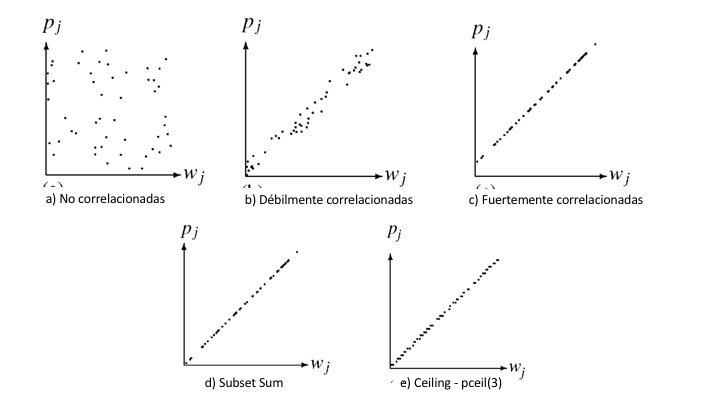
\includegraphics[width=14cm]{images/cap3/correlaciones.jpg}
    \captionof{figure}{Relación entre peso y beneficio de los ítems de la mochila para cada grupo \citep{pisinger_2005}.}\label{fig:correlaciones}
\endgroup

El conjunto de instancias disponibles cuenta con un total de 792 instancias para cada uno de los grupos a utilizar (3960 instancias en total para los cinco grupos mencionados), las que varían entre 50, 100, 200, 500, 1000, 2000, 5000 y 10.000 ítems por instancia de una forma equitativamente distribuida. Es decir, el grupo NC cuenta con 99 instancias que contienen 50 ítems, 99 instancias que contienen 100 ítems, 99 instancias que contienen 200 ítems, 99 instancias que contienen 500 ítems, 99 instancias que contienen 1.000 ítems, 99 instancias que contienen 2.000 ítems, 99 instancias que contienen 5.000 ítems y 99 instancias que contienen 10.000 ítems, y así sucesivamente para cada uno de los grupos. Todas las instancias disponibles cuentan con su valor óptimo y a lo menos una posible solución. Estas instancias pueden ser encontradas en \url{http://www.diku.dk/~pisinger/codes.html}.

Dada la gran cantidad de casos de adaptación, se realiza un experimento utilizando cada uno de los grupos seleccionados, más la adición de un grupo que contenga la mezcla de los demás (GX). Es decir, se realizan seis sub-experimentos dentro de cada uno de los experimentos del PM-01. Estos experimentos utilizan los grupos NC, DC, FC, SS, Ceil y GX, tanto para el experimento 1 como el experimento 2. 

Del total de instancias se ha seleccionado un grupo como caso de adaptación para el proceso evolutivo y otro grupo como evaluación de los algoritmos generados en el proceso evolutivo. Las instancias a evaluar fueron generadas de forma automática con el mismo criterio para cada uno de los grupos descritos, por lo que la selección de instancias utilizadas para cada grupo (evolución y evaluación) es determinada de forma arbitraria. En los casos de adaptación, el número de instancias varía de acuerdo a cada uno de los experimentos 1 y 2, ya que como se mencionó en el capítulo \ref{cap:disegno_experimento}, las instancias es otro factor que varía para el diseño de éstos. El tamaño de las instancias (cantidad de ítems) para los casos de adaptación varía entre 50, 100, 200, 500. Este tamaño del problema claramente una complejidad alta para un experto humano y permite ejecutar la PG en tiempos razonables. Para las instancias de evaluación son utilizados los mismos grupos para ambos experimentos.


\subsection{Conjuntos de instancias de adaptación con co-evolución}
\label{cap:ins_coev}

Para el experimento con co-evolución durante el proceso evolutivo se requieren dos conjuntos de instancias de adaptación. Estos grupos de instancias son diferenciados por su tamaño. Para el grupo 1 se utilizan las instancias de tamaño 200 y 500, mientras que para el grupo 2 se utilizan instancias de tamaño 50 y 100. El número de instancias para cada grupo es de seis instancias, siendo tres de cada uno de los tamaños mencionados. Este número ha sido determinado en trabajos relacionados \citep{contreras_2013, parada_2015} y permite obtener buenos resultados para el proceso evolutivo. En la Tabla \ref{tab:ins_islas} se encuentran las instancias de adaptación para cada uno de los casos. En éstas se puede apreciar que el grupo GX está compuesta por algunas de las instancias pertenecientes a los otros grupos. Por otra parte, las instancias son clasificadas por el nombre del grupo y un correlativo correspondiente a la pertenencia que tengan a los grupos 1 o 2 de instancias. Por ejemplo, NC1 pertenece al grupo NC de clasificación y al grupo 1 de las instancias.

\begin{table}[hbtp!]
\caption{Conjunto de instancias de adaptación para el experimento 2}\label{tab:ins_islas}
\small
\centering
\begin{center}
\begin{tabular}{cc||ccc}
\hline
{\textbf{Grupo}} & {\textbf{Nombre instancia}} & {\textbf{Grupo}} & \multicolumn{2}{c}{{\textbf{Nombre instancia}}} \\ \hline
NC1 & 	\begin{tabular}[c]{@{}l@{}}
						 knapPI\_1\_200\_1000\_26 \\ 
						 knapPI\_1\_200\_1000\_63 \\
						 knapPI\_1\_200\_1000\_8 \\
						 knapPI\_1\_500\_1000\_5 \\
						 knapPI\_1\_500\_1000\_86 \\
						 knapPI\_1\_500\_1000\_94
						\end{tabular} & DC1 & 
										\multicolumn{2}{c}{
											\begin{tabular}[c]{@{}l@{}}
											 knapPI\_2\_200\_1000\_26 \\
											 knapPI\_2\_200\_1000\_63 \\
											 knapPI\_2\_200\_1000\_8 \\
											 knapPI\_2\_500\_1000\_5 \\
											 knapPI\_2\_500\_1000\_86 \\
											 knapPI\_2\_500\_1000\_94
											\end{tabular}}\\
\hline
NC2 & 	\begin{tabular}[c]{@{}l@{}}
						 knapPI\_1\_100\_1000\_19 \\
						 knapPI\_1\_100\_1000\_26 \\
						 knapPI\_1\_100\_1000\_6 \\
						 knapPI\_1\_50\_1000\_19 \\
						 knapPI\_1\_50\_1000\_26 \\
						 knapPI\_1\_50\_1000\_7 
						\end{tabular} & DC2 &
										\multicolumn{2}{c}{
											\begin{tabular}[c]{@{}l@{}}
											 knapPI\_2\_100\_1000\_19 \\
											 knapPI\_2\_100\_1000\_26 \\
											 knapPI\_2\_100\_1000\_6 \\
											 knapPI\_2\_50\_1000\_19 \\
											 knapPI\_2\_50\_1000\_26 \\
											 knapPI\_2\_50\_1000\_7 
											\end{tabular}}\\
\hline
FC1 & 	\begin{tabular}[c]{@{}l@{}}
						 knapPI\_3\_200\_1000\_26 \\
						 knapPI\_3\_200\_1000\_63 \\
						 knapPI\_3\_200\_1000\_8 \\
						 knapPI\_3\_500\_1000\_5 \\
						 knapPI\_3\_500\_1000\_86 \\
						 knapPI\_3\_500\_1000\_94 
						\end{tabular} & SS1 &
										\multicolumn{2}{c}{
											\begin{tabular}[c]{@{}l@{}}
											 knapPI\_6\_200\_1000\_26 \\
											 knapPI\_6\_200\_1000\_63 \\
											 knapPI\_6\_200\_1000\_8 \\
											 knapPI\_6\_500\_1000\_5 \\
											 knapPI\_6\_500\_1000\_86 \\
											 knapPI\_6\_500\_1000\_94 
											\end{tabular}}\\
\hline
FC2 & 	\begin{tabular}[c]{@{}l@{}}
						 knapPI\_3\_100\_1000\_19 \\
						 knapPI\_3\_100\_1000\_26 \\
						 knapPI\_3\_100\_1000\_6 \\
						 knapPI\_3\_50\_1000\_19 \\
						 knapPI\_3\_50\_1000\_26 \\
						 knapPI\_3\_50\_1000\_7 
						\end{tabular} & SS2 & 
										\multicolumn{2}{c}{				
											\begin{tabular}[c]{@{}l@{}}
											 knapPI\_6\_100\_1000\_19 \\
											 knapPI\_6\_100\_1000\_26 \\
											 knapPI\_6\_100\_1000\_6 \\
											 knapPI\_6\_50\_1000\_19 \\
											 knapPI\_6\_50\_1000\_26 \\
											 knapPI\_6\_50\_1000\_7 
											\end{tabular}}\\
\hline
Ceil1 & 	\begin{tabular}[c]{@{}l@{}}
							 knapPI\_15\_200\_1000\_26 \\
							 knapPI\_15\_200\_1000\_63 \\
							 knapPI\_15\_200\_1000\_8 \\
							 knapPI\_15\_500\_1000\_5 \\
							 knapPI\_15\_500\_1000\_86 \\
							 knapPI\_15\_500\_1000\_94
							\end{tabular} & GX1 &  \begin{tabular}[c]{@{}l@{}}
																		 knapPI\_1\_200\_1000\_8 \\
																		 knapPI\_2\_200\_1000\_8 \\
																		 knapPI\_3\_200\_1000\_8 \\
																		 knapPI\_6\_200\_1000\_8 \\
																		 knapPI\_15\_200\_1000\_8
																	\end{tabular} &  \begin{tabular}[c]{@{}l@{}}
																		 knapPI\_1\_500\_1000\_5 \\
																		 knapPI\_2\_500\_1000\_5 \\
																		 knapPI\_3\_500\_1000\_5 \\
																		 knapPI\_6\_500\_1000\_5 \\
																		 knapPI\_15\_500\_1000\_5
																	\end{tabular}\\ 
\hline
Ceil2 & 	\begin{tabular}[c]{@{}l@{}}
							 knapPI\_15\_100\_1000\_19 \\
							 knapPI\_15\_100\_1000\_26 \\
							 knapPI\_15\_100\_1000\_6 \\
							 knapPI\_15\_50\_1000\_19 \\
							 knapPI\_15\_50\_1000\_26 \\
							 knapPI\_15\_50\_1000\_7 
							\end{tabular} & GX2 &  \begin{tabular}[c]{@{}l@{}}
																		 knapPI\_1\_100\_1000\_6 \\
																		 knapPI\_2\_100\_1000\_6 \\
																		 knapPI\_3\_100\_1000\_6 \\
																		 knapPI\_6\_100\_1000\_6 \\
																		 knapPI\_15\_100\_1000\_6
																	\end{tabular} &  \begin{tabular}[c]{@{}l@{}}
																		 knapPI\_1\_50\_1000\_7 \\
																		 knapPI\_2\_50\_1000\_7 \\
																		 knapPI\_3\_50\_1000\_7 \\
																		 knapPI\_6\_50\_1000\_7 \\
																		 knapPI\_15\_50\_1000\_7
																	\end{tabular}\\ 
\hline
\end{tabular}
\end{center}
\caption*{(Elaboración propia, 2015)}
\end{table}


\subsection{Conjuntos de instancias de adaptación sin co-evolución}

El conjunto de instancias de adaptación para el experimento sin co-evolución es la combinación de los grupos 1 y 2 utilizados en \ref{cap:ins_coev} para cada uno de los grupos. En la Tabla \ref{tab:ins_trad} se puede apreciar los grupos y sus respectivas instancias.

\begin{table}[hbtp!]
\caption{Conjunto de instancias de adaptación para el experimento 1}\label{tab:ins_trad}
\small
\centering
\begin{center}
\begin{tabular}{cc||ccc}
\hline
{\textbf{Grupo}} & {\textbf{Nombre instancia}} & {\textbf{Grupo}} & \multicolumn{2}{c}{{\textbf{Nombre instancia}}} \\ \hline
NC & 	\begin{tabular}[c]{@{}l@{}}
						 knapPI\_1\_200\_1000\_26 \\ 
						 knapPI\_1\_200\_1000\_63 \\
						 knapPI\_1\_200\_1000\_8 \\
						 knapPI\_1\_500\_1000\_5 \\
						 knapPI\_1\_500\_1000\_86 \\
						 knapPI\_1\_500\_1000\_94 \\
						 knapPI\_1\_100\_1000\_19 \\
						 knapPI\_1\_100\_1000\_26 \\
						 knapPI\_1\_100\_1000\_6 \\
						 knapPI\_1\_50\_1000\_19 \\
						 knapPI\_1\_50\_1000\_26 \\
						 knapPI\_1\_50\_1000\_7
						\end{tabular} & DC & 
										\multicolumn{2}{c}{
											\begin{tabular}[c]{@{}l@{}}
											 knapPI\_2\_200\_1000\_26 \\
											 knapPI\_2\_200\_1000\_63 \\
											 knapPI\_2\_200\_1000\_8 \\
											 knapPI\_2\_500\_1000\_5 \\
											 knapPI\_2\_500\_1000\_86 \\
											 knapPI\_2\_500\_1000\_94 \\
											 knapPI\_2\_100\_1000\_19 \\
											 knapPI\_2\_100\_1000\_26 \\
											 knapPI\_2\_100\_1000\_6 \\
											 knapPI\_2\_50\_1000\_19 \\
											 knapPI\_2\_50\_1000\_26 \\
											 knapPI\_2\_50\_1000\_7 
											\end{tabular}}\\

\hline
FC & 	\begin{tabular}[c]{@{}l@{}}
						 knapPI\_3\_200\_1000\_26 \\
						 knapPI\_3\_200\_1000\_63 \\
						 knapPI\_3\_200\_1000\_8 \\
						 knapPI\_3\_500\_1000\_5 \\
						 knapPI\_3\_500\_1000\_86 \\
						 knapPI\_3\_500\_1000\_94 \\
						 knapPI\_3\_100\_1000\_19 \\
						 knapPI\_3\_100\_1000\_26 \\
						 knapPI\_3\_100\_1000\_6 \\
						 knapPI\_3\_50\_1000\_19 \\
						 knapPI\_3\_50\_1000\_26 \\
						 knapPI\_3\_50\_1000\_7 
						\end{tabular} & SS &
										\multicolumn{2}{c}{
											\begin{tabular}[c]{@{}l@{}}
											 knapPI\_6\_200\_1000\_26 \\
											 knapPI\_6\_200\_1000\_63 \\
											 knapPI\_6\_200\_1000\_8 \\
											 knapPI\_6\_500\_1000\_5 \\
											 knapPI\_6\_500\_1000\_86 \\
											 knapPI\_6\_500\_1000\_94 \\
											 knapPI\_6\_100\_1000\_19 \\
											 knapPI\_6\_100\_1000\_26 \\
											 knapPI\_6\_100\_1000\_6 \\
											 knapPI\_6\_50\_1000\_19 \\
											 knapPI\_6\_50\_1000\_26 \\
											 knapPI\_6\_50\_1000\_7 
											\end{tabular}}\\
\hline
Ceil & 	\begin{tabular}[c]{@{}l@{}}
							 knapPI\_15\_200\_1000\_26 \\
							 knapPI\_15\_200\_1000\_63 \\
							 knapPI\_15\_200\_1000\_8 \\
							 knapPI\_15\_500\_1000\_5 \\
							 knapPI\_15\_500\_1000\_86 \\
							 knapPI\_15\_500\_1000\_94 \\
							 knapPI\_15\_100\_1000\_19 \\
							 knapPI\_15\_100\_1000\_26 \\
							 knapPI\_15\_100\_1000\_6 \\
							 knapPI\_15\_50\_1000\_19 \\
							 knapPI\_15\_50\_1000\_26 \\
							 knapPI\_15\_50\_1000\_7 
							\end{tabular} & GX1 &  \begin{tabular}[c]{@{}l@{}}
																		 knapPI\_1\_200\_1000\_8 \\
																		 knapPI\_2\_200\_1000\_8 \\
																		 knapPI\_3\_200\_1000\_8 \\
																		 knapPI\_6\_200\_1000\_8 \\
																		 knapPI\_15\_200\_1000\_8 \\
																		 knapPI\_1\_100\_1000\_6 \\
																		 knapPI\_2\_100\_1000\_6 \\
																		 knapPI\_3\_100\_1000\_6 \\
																		 knapPI\_6\_100\_1000\_6 \\
																		 knapPI\_15\_100\_1000\_6
																	\end{tabular} &  \begin{tabular}[c]{@{}l@{}}
																		 knapPI\_1\_500\_1000\_5 \\
																		 knapPI\_2\_500\_1000\_5 \\
																		 knapPI\_3\_500\_1000\_5 \\
																		 knapPI\_6\_500\_1000\_5 \\
																		 knapPI\_15\_500\_1000\_5 \\
																		 knapPI\_1\_50\_1000\_7 \\
																		 knapPI\_2\_50\_1000\_7 \\
																		 knapPI\_3\_50\_1000\_7 \\
																		 knapPI\_6\_50\_1000\_7 \\
																		 knapPI\_15\_50\_1000\_7
																	\end{tabular}\\ 
\hline
\end{tabular}
\end{center}
\caption*{(Elaboración propia, 2015)}
\end{table}

\subsection{Conjunto de instancias de evaluación}

Los grupos de instancias de evaluación tienen por objetivo medir el rendimiento de los algoritmos generados por el proceso evolutivo en un ambiente distinto al de adaptación. Los grupos están compuestos por todas las instancias restantes que no hayan sido utilizadas en el proceso de adaptación. Es decir, cada uno de los grupos está compuesto por 780 instancias de evaluación. Las instancias para el grupo GX están compuestas por todas las instancias de evaluación de los otros grupos.

\section{Parámetros}

Los parámetros a utilizar fueron fijados siguiendo las pautas arrojadas por experimentos preliminares. Estos valores se encuentran basados en otros trabajos que utilizan la PG \citep{drake_2014, parada_2015, contreras_2013} y siguiendo los valores teóricos mencionados en \citep{karafotias_2015, karafotias_2014}. La lista completa con los valores para ambos experimentos se presenta en la Tabla \ref{tab:param_exp1_exp2}. Entre los valores listados en la Tabla se incluyen los relacionados a las islas o poblaciones especificados en \ref{cap:consideraciones}. Los valores de ambos experimentos son similares para realizar una experimentación acorde que permita confirmar o refutar la Hipótesis de este trabajo.

\begin{table}[hbt!]
\caption{Resumen de parámetros para experimentos 1 y 2}\label{tab:param_exp1_exp2}
\small
\centering
\rowcolors{2}{gray!25}{white}
\begin{tabular}{lcc}
\hline
{\textbf{Datos}} & {\textbf{\begin{tabular}[c]{@{}c@{}}Experimento con \\co-evolución\end{tabular}}} & {\textbf{\begin{tabular}[c]{@{}c@{}}Experimento sin \\co-evolución\end{tabular}}} \\ \hline
Número de poblaciones                     &  $4^{*}$                               &  $1^{**}$  \\
Tamaño de población                       &  125 por cada población                &  500 \\
Número de generaciones                    &  \multicolumn{2}{c}{300} \\
Probabilidad de cruzamiento               &  \multicolumn{2}{c}{80\%} \\
Probabilidad de reproducción              &  \multicolumn{2}{c}{10\%} \\
Probabilidad de mutación                  &  \multicolumn{2}{c}{5\% \textit{subtree mutation} y 5\% \textit{one node mutation}} \\
\begin{tabular}[l]{@{}l@{}}
  Método de generación de \\
población inicial 
\end{tabular}                             &  \multicolumn{2}{c}{\textit{Ramped Half and Half}} \\
Método de selección de individuos         &  \multicolumn{2}{c}{Torneo con 4 individuos} \\
Método de selección de nodos              &  \multicolumn{2}{c}{\textit{Koza Node Selector}} \\
Probabilidad de selección de nodos        &  \multicolumn{2}{c}{90\% terminales y 10\% funciones} \\
Altura máxima de evolución                &  \multicolumn{2}{c}{15} \\
Criterio de término                       &  \multicolumn{2}{c}{Completar todas las generaciones} \\
\begin{tabular}[l]{@{}l@{}}
  Individuos a compartir con otra \\
  población
\end{tabular}                             &  5 (son replicados y compartidos)      & no aplica \\
Poblaciones a las que compartir           &  \begin{tabular}[c]{@{}c@{}}Cada población comparte \\con todas las demás \end{tabular} & no aplica \\
\begin{tabular}[l]{@{}l@{}}
  Número de generaciones que la \\          
  población espera para enviar \\
  inmigrantes
\end{tabular}                             &  10                                    & no aplica  \\
\begin{tabular}[l]{@{}l@{}}
  Generación en la que se inicia \\
  el envío de inmigrantes
\end{tabular}                             &  1                                     & no aplica  \\
Selección de inmigrantes a enviar         &  Torneo con 4 individuos               & no aplica  \\
Selección de individuos a eliminar        &  \begin{tabular}[c]{@{}c@{}}
                                              Torneo inverso con 4 \\
                                              individuos
                                             \end{tabular}                         & no aplica  \\

\hline
\end{tabular}
%\caption*{(Elaboración propia, 2015)}
\end{table}


Las cuatro poblaciones están compuestas por la combinación de las funciones objetivo y grupos de instancias de evolución, siendo estos los siguientes:

\begin{itemize}
	\item Población 1: utiliza la función de evaluación $fe_{2}$ y el grupo de instancias G2\_X.
	\item Población 2: utiliza la función de evaluación $fe_{1}$ y el grupo de instancias G1\_X.
	\item Población 3: utiliza la función de evaluación $fe_{1}$ y el grupo de instancias G2\_X.
	\item Población 3: utiliza la función de evaluación $fe_{2}$ y el grupo de instancias G1\_X.
\end{itemize}

La población única está compuesta por la función de evaluación $fe$ y el grupo de instancias G3\_X, siendo \_X el nombre del grupo de instancias correspondiente al sub-experimento de acuerdo a los grupos NC, DC, FC, SS, Ceil y GX, como se menciona en \ref{cap:sel_casos_adapt_pm01}.

\section{El proceso evolutivo}

Para llevar a cabo los experimentos, se realizan los 6 sub-experimentos ya mencionados para cada uno de los experimentos correspondientes al PM-01. Estos sub-experimentos corresponden a la ejecución de cada uno de los métodos con el grupo de instancias correspondiente. En la Tabla \ref{tab:resumen_exp} es posible apreciar cada uno de los experimentos, los cuales son ejecutados cinco veces cada uno. Todos los demás elementos requeridos en el proceso evolutivo son los especificados en las secciones anteriores del capítulo \ref{cap:disegno_pm01}.

\begin{table}[hbtp!]
\caption{Resumen nombre de los sub-experimentos de cada experimento del PM-01}\label{tab:resumen_exp}
\small
\centering
\begin{center}
\rowcolors{2}{gray!25}{white}
\begin{tabular}{cc||cc}
\hline
\multicolumn{2}{c||}{{\textbf{Experimento 1}}} & \multicolumn{2}{c}{{\textbf{Experimento 2}}} \\
{\textbf{Grupo instancias}} & {\textbf{Nombre exp.}} & {\textbf{Grupo instancias}} & {\textbf{Nombre exp.}} \\ \hline
G3\_NC   & Experimento 1.a & G1\_NC $\cup$ G2\_NC 		& Experimento 2.a \\
G3\_DC   & Experimento 1.b & G1\_DC $\cup$ G2\_DC 		& Experimento 2.b \\
G3\_FC   & Experimento 1.c & G1\_FC $\cup$ G2\_FC 		& Experimento 2.c \\
G3\_SS   & Experimento 1.d & G1\_SS $\cup$ G2\_SS 		& Experimento 2.d \\
G3\_Ceil & Experimento 1.e & G1\_Ceil $\cup$ G2\_Ceil 	& Experimento 2.e \\
G3\_GX   & Experimento 1.f & G1\_GX $\cup$ G2\_DCGX 	& Experimento 2.f \\
\hline
\end{tabular}
\end{center}
\caption*{(Elaboración propia, 2015)}
\end{table}


\chapter{DISEÑO EXPERIMENTO PVV}
\label{cap:disegno_pvv}

%DESCOMENTAR ESTAS LÍNEAS SI EL CAPÍTULO TIENE FIGURAS O TABLAS
% \addtocontents{lof}{{\bf \noindent Figuras del capítulo \arabic{chapter}}}
\addtocontents{lot}{{\bf \noindent Tablas del capítulo \arabic{chapter}}}

En este capítulo se describen en conjunto los experimentos 3 y 4 correspondientes al PVV. Estos experimentos poseen gran parte de su estructura en común y las diferencias son especificadas en cada una de las secciones correspondientes.

\section{Estructura de datos}

Los algoritmos generados se construyen utilizando varias estructuras de datos. Estas estructuras se diseñaron en base al modelo matemático y a las funciones y terminales que operan sobre ellas. Se dividen en dos clases: estructuras variables y estructuras fijas.

\subsection{Estructura de datos variables}

Las estructuras variables mantienen la información de las ciudades que han sido ingresadas al circuito y las ciudades que aún restan por ingresar y una matriz completa de las distancias. Estas estructuras varían de acuerdo a la acción que realicen los terminales, son las siguientes:

\begin{itemize}
	\item Lista de ciudades disponibles (LCD): lista que contiene todas las ciudades disponibles para trabajar en el problema, las ciudades pertenecientes a esta lista varían de acuerdo al proceso de la solución. Esta lista se inicializa con todas las ciudades disponibles por la instancia del problema.
	\item Lista de ciudades agregadas (LCA): lista que contiene todas las ciudades agregadas al circuito en algún instante del proceso. Esta lista se encuentra vacía al momento de inicializar el proceso de obtención de la solución.
\end{itemize}

Sobre estas listas solo se pueden realizar dos acciones: agregar o remover una ciudad. Toda acción realizada sobre una de ellas, repercute de forma inversa en la otra. Es decir, si se agrega una ciudad en LCD, se debe quitar de forma inmediata de LCA.

\subsection{Estructura de datos fijas}

Las estructuras fijas son creadas al momento de iniciar el proceso evolutivo. Son utilizadas por los terminales para poder realizar las acciones que éstos tengan definidas, donde cada una de estas estructuras es inicializada de acuerdo a los valores que se obtienen de las instancias. A continuación se presenta el detalle de éstas:

\begin{itemize}
	\item Matriz de costos (MC): lista de listas que contiene la matriz completa de distancias. En esta matriz se encuentran los costos de viajar de cada una de las ciudades a otra. Esta es inicializada al momento de iniciar el proceso evolutivo.
	\item Ciudades cercanas al centro (CCC): lista que contiene de forma ordenada la mitad de las ciudades cercanas al centro. El orden de éstas está dado por las más cercanas a las más lejanas.
	\item Ciudades lejanas al centro (CLC): lista que contiene de forma ordenada la mitad de las ciudades cercanas al centro. Esta lista es el complemento de la lista de CCC. El orden de éstas está dado por las más lejanas a las más cercanas.
	\item Valor óptimo de la instancia: contiene el valor óptimo del beneficio de la instancia.
	\item Total de ciudades: contiene el número de ciudades del circuito.
	\item Peor arco: contiene el valor del peor arco de la instancia.
\end{itemize}

\section{Funciones y terminales}

Las funciones y terminales son las operaciones elementales sobre las estructuras de datos anteriormente definidas. La definición de éstos permite realizar las operaciones sobre las estructuras definidas con el objetivo de completar el circuito de costo mínimo que utilice todas las ciudades. Se construyen terminales en base a heurísticas existentes para el PVV, y funciones que permitan operar en diversas combinaciones sobre estos terminales.

Los elementos del conjunto de funciones y terminales deben cumplir con las propiedades de suficiencia y clausura \citep{poli_2008}. Las funciones y terminales cumplen la propiedad de clausura, ya que todas retornan un valor verdadero o falso, y las funciones solo pueden recibir parámetros de entrada de ese tipo. Los terminales utilizados están basados en heurísticas del PVV,en su conjunto proveen variabilidad de algoritmos que permiten solucionar el problema, es con esto que se cumple la propiedad de suficiencia. 

\subsection{Conjunto de funciones}

Las funciones que conforman los algoritmos generados contienen instrucciones básicas utilizadas en su mayoría por todos los lenguajes de programación. Desde el punto de vista de la PG, las funciones corresponden a los nodos internos del árbol \citep{koza_poli_2005}. En la Tabla \ref{tab:func_pvv} se muestran las funciones utilizadas, éstas son las mismas utilizadas en los experimentos correspondientes al PM-01.

\begin{table}[hbt!]
\caption{Grupo de funciones para el PVV}\label{tab:func_pvv}
\small
\centering
\rowcolors{2}{gray!25}{white}
\begin{tabular}{lcl}
\hline
{\textbf{Nº}} & {\textbf{Nombre}} & {\textbf{Descripción}} \\ \hline
1	& $while(A, B)$				&	\begin{tabular}[c]{@{}l@{}}
										Mientras la expresión A sea Verdadera se ejecuta la instrucción B. \\
										Tiene como límite de iteraciones que el valor del beneficio no varíe \\
										en tres iteraciones.\\ 
										Devuelve verdadero en caso de realizar una o más iteraciones y \\
										falso en caso contrario.
									\end{tabular} \\
2	& $IfThenElse(A, B, C)$		&	\begin{tabular}[c]{@{}l@{}}
										Ejecuta B si A es verdadero y C si A es falso. \\
										Devuelve el valor de B o C según sea el caso.
									\end{tabular} \\
3	& $IfThen(A, B)$			&	\begin{tabular}[c]{@{}l@{}}
										Ejecuta B si A es verdadero.\\
										Devuelve verdadero si logra ejecutar B al menos una vez y \\
										devuelve falso en caso contrario.
									\end{tabular} \\
4	& $Not(A)$					&	\begin{tabular}[c]{@{}l@{}}
										Función lógica que implementa la negación lógica. \\
										Devuelve verdadero si A es falso y devuelve falso si A \\
										es verdadero.
									\end{tabular} \\
5	& $And(A, B)$				&	\begin{tabular}[c]{@{}l@{}}
										Función lógica que implementa la conjunción lógica. \\
										Devuelve verdadero si A y B son verdaderos y devuelve falso \\
										en los otros casos.
									\end{tabular} \\
6	& $Or(A, B)$				&	\begin{tabular}[c]{@{}l@{}}
										Función lógica que implementa la disyunción lógica. \\
										Devuelve verdadero si A o B son verdaderos y devuelve falso \\
										en los otros casos.
									\end{tabular} \\
7	& $Equal(A, B)$				&	\begin{tabular}[c]{@{}l@{}}
										Función que compara la igualdad de A y B. \\
										Devuelve verdadero si A y B son iguales y devuelve falso \\
										en caso contrario.
									\end{tabular} \\
\hline
\end{tabular}
%\caption*{(Elaboración propia, 2015)}
\end{table}

\subsection{Conjunto de terminales}

Los terminales son funciones diseñadas para el PVV, los que permiten agregar ciudades o elementos de la lista de ciudades disponibles a la lista de ciudades agregadas de acuerdo a algún criterio establecido. Cada uno de los terminales es una heurística elemental capaz de modificar la estructura de datos definida generando nuevas soluciones. Se ha restringido a los terminales para que no puedan generar soluciones infactibles para el problema, es decir, no es posible generar soluciones que no cumplan alguna de las restricciones propias del problema.

Los terminales utilizados son componentes elementales de las heurísticas descritas en la sección \ref{cap:rev_lit_pvv}, es decir, representan una acción mínima de alguna de las heurísticas que permiten realizar alguna acción para completar el circuito del PVV. Éstos son descritos en la Tabla \ref{tab:term_pvv}.

\begin{table}[hbtp!]
\caption{Grupo de terminales para el PVV}\label{tab:term_pvv}
\small
\centering
\rowcolors{2}{gray!25}{white}
\begin{tabular}{lcl}
\hline
{\textbf{Nº}} & {\textbf{Nombre}} & {\textbf{Descripción}} \\ \hline
1	& AgregarMejorVecino			&	\begin{tabular}[c]{@{}l@{}}
											Busca en la lista de ciudades disponibles, la ciudad que agregue el \\
											menor costo al circuito al ser agregada al final de éste. Si encuentra \\
											una ciudad (si el circuito no está completo), ésta es agregada al \\
											final del circuito. \\
											Retorna verdadero si agrega la ciudad, falso en caso contrario.
										\end{tabular} \\
2	& AgregarPeorVecino				&	\begin{tabular}[c]{@{}l@{}}
											Busca en la lista de ciudades disponibles, la ciudad que agregue el \\
											mayor costo al circuito al ser agregada al final de éste. Si encuentra \\
											una ciudad (si el circuito no está completo), ésta es agregada al \\
											final del circuito. \\
											Retorna verdadero si agrega la ciudad, falso en caso contrario.
										\end{tabular} \\
3	& AgregarCercaCentro			&	\begin{tabular}[c]{@{}l@{}}
											Busca la ciudad más cercana a las coordenadas del centro que se \\
											encuentre disponible. Si encuentra una ciudad (si el circuito no está \\
											completo), ésta es agregada al final del circuito. \\
											Retorna verdadero si agrega la ciudad, falso en caso contrario.
										\end{tabular} \\
4	& AgregarLejosCentro			&	\begin{tabular}[c]{@{}l@{}}
											Busca la ciudad más lejana a las coordenadas del centro que se \\
											encuentre disponible. Si encuentra una ciudad (si el circuito no está \\
											completo), ésta es agregada al final del circuito. \\
											Retorna verdadero si agrega la ciudad, falso en caso contrario.
										\end{tabular} \\
5	& AgregarCercano				&	\begin{tabular}[c]{@{}l@{}}
											Busca la ciudad que al ser insertada en cualquier posición del \\
											circuito, agregue el menor costo a éste. Por ejemplo, se tiene el circuito \\
											$[A, B, C]$ donde ingresa $D$, siendo $A->D < B->D < C->D$. El \\
											resultado luego de la inserción es $[A, D, B, C]$. \\
											Retorna verdadero si agrega la ciudad, falso en caso contrario.
										\end{tabular} \\
6	& AgregarLejano					&	\begin{tabular}[c]{@{}l@{}}
											Busca la ciudad que al ser insertada en cualquier posición del \\
											circuito, agregue el mayor costo a éste. Por ejemplo, se tiene el circuito \\
											$[A, B, C]$ donde ingresa $D$, siendo $A->D < B->D < C->D$. El \\
											resultado luego de la inserción es $[A, B, C, D]$. \\
											Retorna verdadero si agrega la ciudad, falso en caso contrario.
										\end{tabular} \\
7	& AgregarArcoMenor				&	\begin{tabular}[c]{@{}l@{}}
											De forma similar a agregar cercano, busca una ciudad que al ser \\
											insertada agregue el menor costo al circuito. La diferencia está en \\
											que el menor costo es considerando el nuevo arco a formar. Por \\
											ejemplo, se tiene el circuito $[A, B, C]$ y se agrega $X$, \\
											siendo $A->X->B > B->X->C > C->X$. El resultado \\
											es $[A, X, B, C]$. \\
											Retorna verdadero si agrega la ciudad, falso en caso contrario.
										\end{tabular} \\

\hline
\end{tabular}
%\caption*{(Elaboración propia, 2015)}
\end{table}

\addtocounter{table}{-1}
\begin{table}[hbtp!]
\caption{Grupo de terminales para el PVV (continuación)}\label{tab:term_pvv_2}
\small
\centering
\rowcolors{2}{gray!25}{white}
\begin{tabular}{lcl}
\hline
{\textbf{Nº}} & {\textbf{Nombre}} & {\textbf{Descripción}} \\ \hline
8	& AgregarArcoMayor				&	\begin{tabular}[c]{@{}l@{}}
											De forma similar a agregar lejano, busca una ciudad que al ser \\
											insertada agregue el mayor costo al circuito. La diferencia en este \\
											caso se encuentra en que el mayor costo considera el nuevo \\
											arco a formar. Por ejemplo, se tiene el circuito $[A, B, C]$ y se agrega \\
											$X$, siendo $A->X->B < B->X->C < C->X$. \\
											El resultado es $[A, B, C, X]$.
										\end{tabular} \\
9	& Invertir						&	\begin{tabular}[c]{@{}l@{}}
											Cambia el orden de las ciudades sólo en el caso en que este \\
											cambio produzca alguna mejora. El cambio se realiza mediante la \\
											inversión de las posiciones de los extremos hacia adentro. Por \\
											ejemplo, la primera se invierte con la última, la segunda con \\
											la penúltima y así sucesivamente. \\
											Retorna verdadero si logra mejorar el costo del circuito y \\
											falso en caso contrario.
										\end{tabular} \\
10	& EliminarPeorArco				&	\begin{tabular}[c]{@{}l@{}}
											Busca en el circuito dos ciudades que produzcan el peor arco \\
											(el mayor costo al circuito). Ambas ciudades correspondientes \\
											al peor arco son eliminadas. \\
											Retorna verdadero si logra eliminar el arco y falso en caso\\
											contrario.
										\end{tabular} \\
11	& EliminarPeorNodo\_i			&	\begin{tabular}[c]{@{}l@{}}
											Busca en el circuito dos ciudades que produzcan el peor arco \\
											(el mayor costo al circuito). Sólo es eliminada la ciudad que \\
											inicia el arco. \\
											Retorna verdadero si logra eliminar el arco y falso en caso \\
											contrario.
										\end{tabular} \\
12	& EliminarPeorNodo\_j			&	\begin{tabular}[c]{@{}l@{}}
											Busca en el circuito dos ciudades que produzcan el peor arco \\
											(el mayor costo al circuito). Sólo es eliminada la ciudad que \\
											termina el arco. \\
											Retorna verdadero si logra eliminar el arco y falso en caso \\
											contrario.
										\end{tabular} \\
13	& 2-opt							&	\begin{tabular}[c]{@{}l@{}}
											Optimizador que utiliza la heurística \textit{2-opt}. \\
											Retorna verdadero si puede realizar alguna mejora al circuito \\
											y falso en caso contrario.
										\end{tabular} \\
\hline
\end{tabular}
\caption*{(Elaboración propia, 2015)}
\end{table}

Dentro de los terminales descritos en la Tabla \ref{tab:term_pvv}, el terminal \textit{“2-opt”} es siempre utilizado, tanto en las pruebas preliminares como en otros trabajos que utilizan este terminal, por lo que éste se utiliza como parte de la estructura fija que tienen los algoritmos \citep{sepulveda_2011}, es decir, es parte de la estructura de todos los algoritmos generados para los experimentos 3 y 4.

\section{Función de evaluación}
\label{cap:func_eval_pvv}

La función de evaluación es el mecanismo primario para comunicar la declaración de alto nivel de los requisitos del problema con el sistema de PG \citep{koza_poli_2005}. En el capítulo \ref{cap:disegno_experimento} se muestra que los experimentos 3 y 4 difieren en la función de evaluación que utilizan. En el caso de la PG tradicional, se utiliza una función de evaluación compuesta por las dos funciones de evaluación utilizadas en el experimento de las islas. La función de evaluación para cada uno de los experimentos tiene por objetivo medir la calidad de los algoritmos y su legibilidad desde el punto de vista de un humano. La calidad está dada por “que tan bien resuelve el algoritmo el problema”, es decir, que tan “cerca” estoy del valor óptimo. La legibilidad está dada por “que tan fácil es leer, entender y ejecutar el algoritmo por un humano”. La estructura de los algoritmos generados es representada por nodos de un árbol sintáctico, siendo estos nodos los terminales y funciones. Mientras menor sea la cantidad de nodos es más fácil leer el algoritmo representado por el árbol sintáctico. Por lo tanto, la legibilidad de un algoritmo se considera como opuesta al tamaño de éste.

La calidad de los algoritmos es el factor que varía entre las distintas funciones objetivos de los experimentos, mientras que la legibilidad es una función común a todos los casos. Estos factores de calidad y legibilidad son considerados de forma compuesta para la función de evaluación que es utilizada en cada uno de los experimentos. A diferencia de las funciones de evaluación utilizadas en los experimentos relacionados al PM-01, en las relacionadas al PVV no se utilizan factores de relevancia. Adicionalmente, para el PVV no es posible restringir infactibilidades por medio de los terminales, lo que obliga a incluir un factor penalización si las soluciones entregadas por un algoritmo no son factibles. Finalmente, las funciones de evaluación de para los experimentos relacionados a este problema están compuestas por las ecuaciones que representen la calidad, el factor de legibilidad y la penalización del algoritmo. Tanto la función de legibilidad como de penalización son la misma para ambos experimentos.

La función de legibilidad $leg_{p}$ para el algoritmo $p$ está dada por la ecuación (\ref{eq:leg_pvv}).Donde $N_{p}$ es el número de nodos del algoritmo $p$, mientras que $M_{p}$ es el número máximo de nodos permitidos para los algoritmos.

\begin{equation}
\label{eq:leg_pvv}
	leg_{p} = 	\begin{cases}
					0       & \quad \text{si } N_{p} \leq M_{p} \\
					\frac{M_{p}-N_{p}}{M_{p}}  & \quad \text{si } N_{p} > M_{p}\\
				\end{cases}
\end{equation}

El factor de penalización se compone del producto del error relativo del número de ciudades (ERC) representado por la ecuación (\ref{eq:ERC_pvv}) con el promedio del peor arco (PPA) representado por la ecuación (\ref{eq:PPA_pvv}). Siendo $ERC_{s}$ el error relativo del número de ciudades para el conjunto de instancias $S$, $c_{i}$ el número de ciudades actualmente ingresadas por el algoritmo $p$ en la instancia $i$ y $x_{i}$ el número de total ciudades de la instancia $i$. $PPA_{s}$ representa promedio del peor arco para el conjunto de instancias $S$, donde $e_{i}$ es el peor arco de la instancia $i$.

\begin{equation}
\label{eq:ERC_pvv}
	ERC_{s} = \frac{1}{n_{s}} \cdot \sum\limits_{i=1}^{n_{s}} \frac{x_{i} - c_{i}}{x_{i}} 
\end{equation}

\begin{equation}
\label{eq:PPA_pvv}
	PPA_{s} = \frac{1}{n_{s}} \cdot \sum\limits_{i=1}^{n_{s}} e_{i}
\end{equation}

\subsection{Función de evaluación experimento con co-evolución}

Para el experimento con co-evolución, durante el proceso evolutivo se requieren dos funciones de evaluación que cumplan con evaluar la calidad de los algoritmos de acuerdo al problema. Para esto se utilizan las siguientes funciones de evaluación.

Función de evaluación de la calidad por medio del ERP: Como se mencionó en las secciones \ref{cap:experimento_tradicional} y \ref{cap:experimento_islas}, el ERP consiste en el error relativo promedio de los algoritmos obtenidos. Para cada grupo de instancias de evaluación $S$, se determina el porcentaje promedio por el cual el beneficio obtenido $o_{i}$ se encuentra distanciado de la mejor solución $z_{i}$ para cada instancia del conjunto $S$. Esto se representa en la siguiente ecuación (\ref{eq:ERP_pvv}), donde $n_{s}$ representa el número de instancias del conjunto $S$.

\begin{equation}
\label{eq:ERP_pvv}
	ERP_{s} =  \frac{1}{n_{s}} \cdot \sum\limits_{i=1}^{n_{s}} \frac{\|z_{i} - o_{i}\|}{z_{i}} 
\end{equation}

Función de evaluación de la calidad por medio de los HITS: esta función de evaluación representa que tantas instancias $i$ del conjunto $S$ evaluadas con el algoritmo $p$ obtienen un error relativo menor a $0,05$ ($5\%$). La ecuación (\ref{eq:ER_pvv}) representa el ER de la instancia $i$, el cual es utilizado en la ecuación (\ref{eq:HIT_pvv}) para determinar si el resultado de éste es $1$ o $0$. Finalmente la ecuación (\ref{eq:HITS_pvv}) utiliza los resultados obtenidos en la evaluación de cada una de las instancias $i$ por la ecuación (\ref{eq:HIT_pvv}) para calcular el número de \textit{hits} (aciertos) que obtiene el algoritmo $p$.

\begin{equation}
\label{eq:ER_pvv}
	ER_{i} = \frac{\|z_{i}-o{i}\|}{z_{i}}
\end{equation}

\begin{equation}
\label{eq:HIT_pvv}
	HIT_{i} = 	\begin{cases}
					1       & \quad \text{si } ER_{i} \leq 5\% \\
					0  		& \quad \text{si } ER_{i} > 5\%	   \\
				\end{cases}
\end{equation}

\begin{equation}
\label{eq:HITS_pvv}
	HITS_{s} = 	\frac{n_{s} - \sum\limits_{i=1}^{n_{s}} HIT_{i} }{n_{s}}
\end{equation}

Para obtener las funciones de evaluación para el experimento 4 es necesario combinar los factores de calidad, legibilidad y penalización. Éstas funciones de evaluación quedan representadas por las ecuaciones (\ref{eq:f1_islas_pvv}) y (\ref{eq:f2_islas_pvv}).

\begin{equation}
\label{eq:f1_islas_pvv}
	fe_{3} = ERP_{s} + leg_{p} + ERC_{s} \cdot PPA_{s}
\end{equation}

\begin{equation}
\label{eq:f2_islas_pvv}
	fe_{4} = HITS_{s} + leg_{p} + ERC_{s} \cdot PPA_{s}
\end{equation}


\subsection{Función de evaluación experimento sin co-evolución}

Para el experimento sin co-evolución o tradicional, durante el proceso evolutivo se utiliza una función objetivo combinada de las funciones (\ref{eq:ERP_pvv}) y (\ref{eq:HITS_pvv}) de acuerdo a lo mencionado en la sección \ref{cap:experimento_islas}. La ecuación (\ref{eq:comb_trad_pvv}) representa la combinación de las ecuaciones mencionadas, siendo $\alpha$ y $\beta=(1-\alpha)$ los factores de relevancia para cada uno de los parámetros de la función.

\begin{equation}
\label{eq:comb_trad_pvv}
	fe_{pvv} = \alpha\cdot ERP_{s}+ \beta\cdot HITS_{s}
\end{equation}

Como se menciona al inicio de esta sección (\ref{cap:func_eval_pvv}) la función de evaluación está dada por la composición de la evaluación de la calidad, legibilidad y penalización por infactibilidades, por lo que a la ecuación (\ref{eq:comb_trad_pvv}) es necesario agregarle el factor de legibilidad y los elementos que componen la penalización, como resultado de la combinación de estos tres factores se obtiene la ecuación (\ref{eq:final_trad_pvv}).

\begin{equation}
\label{eq:final_trad_pvv}
	fe = (\alpha\cdot ERP_{s}+ \beta\cdot HITS_{s}) + leg_{p} + ERC_{s} + PPA_{s}
\end{equation}


\section{Selección casos de adaptación}
\label{cap:sel_casos_adapt_pvv}

Los casos de adaptación (instancias) para el problema fueron extraídos de la TSPLIB, que consiste en una librería con distintos casos de prueba del PVV. Esta librería ha sido ampliamente utilizada en trabajos relacionados a este problema utilizando diversos métodos y no solo de PG. Algunas de las instancias disponibles en la librería poseen el circuito óptimo. Adicionalmente, estas instancias poseen el valor del costo mínimo del circuito. El conjunto de instancias extraído cuenta con un total de 53 instancias, las que varían con un mínimo de 42 ciudades y un máximo de 783 ciudades. Las instancias pueden ser extraídas de \url{http://comopt.ifi.uni-heidelberg.de/software/TSPLIB95/tsp/}.

Del total de instancias se ha seleccionado un grupo como caso de adaptación para el proceso evolutivo y otro grupo para la evaluación de los algoritmos generados en el proceso evolutivo. Las instancias disponibles para el problema varían en tamaño, por lo que para la evolución se utilizan instancias que no tengan más de 500 ciudades o nodos. La razón de este criterio para la división se debe a que el proceso evolutivo es lento para este problema tardando aproximadamente 24 horas por ejecución. En los casos de adaptación, el número de instancias varía de acuerdo a cada uno de los experimentos 3 y 4, ya que como se mencionó en el capítulo \ref{cap:disegno_experimento}, las instancias es otro factor que varía para el diseño de éstos. El tamaño de las instancias (cantidad de ciudades) para los casos de adaptación varía con un mínimo de 52 y un máximo de 192. Para las instancias de evaluación, son utilizadas las instancias restantes.

\subsection{Conjuntos de instancias de adaptación con co-evolución}
\label{cap:ins_trad_pvv}

Para el experimento con co-evolución, durante el proceso evolutivo se requieren dos conjuntos de instancias de adaptación. Estos grupos de instancias son diferenciados por su coeficiente de correlación \citep{smith_2012}. Este coeficiente determina la cantidad de diferencias existentes en las distancias de la matriz de costos o distancias entre las ciudades, es decir, si una instancia posee 48 ciudades, tiene una matriz de 2304 elementos. Si estos elementos tuviesen $1.033$ diferencias, tiene un coeficiente de $0,5561$. Para el grupo 1 de instancias se utilizan las instancias que tengan un coeficiente mayor a $0,9$, mientras que para el grupo 2 se utilizan instancias de con un coeficiente entre $0,6$ y $0,8$. El número de instancias para cada grupo es de 9 instancias. Este número ha sido determinado en trabajos relacionados \citep{parada_2015, contreras_2013} y permite obtener bueno resultados para el proceso evolutivo. En la Tabla \ref{tab:ins_islas_pvv} se encuentran las instancias de adaptación divididas por isla.

\begin{table}[hbt!]
\caption{Conjunto de instancias de adaptación proceso evolutivo del experimento 4}\label{tab:ins_islas_pvv}
\small
\centering
\begin{center}
\begin{tabular}{cccc}
\hline
{\textbf{Grupo Instancias}} & {\textbf{Nombre }} & {\textbf{Nº Ciudades}} & {\textbf{Coeficiente correlación}} \\ \hline
Grupo 1 & 	\begin{tabular}[c]{@{}l@{}}
								pr124 \\
								berlin52 \\
								kroC100 \\
								kroE100 \\
								kroA100 \\
								kroB100 \\
								pr76 \\
								kroD100 \\
								lin105
							\end{tabular} & \begin{tabular}[c]{@{}l@{}}
												124 \\
												52 \\
												100 \\
												100 \\
												100 \\
												100 \\
												76 \\
												100 \\
												105 \\
											\end{tabular} & 
													\begin{tabular}[c]{@{}l@{}}
													 	$0.6828$ \\
														$0.7016$ \\
														$0.7349$ \\
														$0.7354$ \\
														$0.7395$ \\
														$0.7404$ \\
														$0.7413$ \\
														$0.7467$ \\
														$0.8142$
													\end{tabular}\\
\hline
Grupo 2 				& 	\begin{tabular}[c]{@{}l@{}}
								pr136 \\
								ch130 \\
								ch150 \\
								eil51 \\
								st70 \\
								rat99 \\
								eil76 \\
								eil101 \\
								rat195
							\end{tabular} & \begin{tabular}[c]{@{}l@{}}
												136 \\
												130 \\
												150 \\
												51 \\
												70 \\
												99 \\
												76 \\
												101 \\
												195
											\end{tabular} & 
													\begin{tabular}[c]{@{}l@{}}
													 	$0.9423$ \\
														$0.9535$ \\
														$0.9652$ \\
														$0.9712$ \\
														$0.9757$ \\
														$0.9783$ \\
														$0.9860$ \\
														$0.9914$ \\
														$0.9922$
													\end{tabular}\\
\hline
\end{tabular}
\end{center}
\caption*{(Elaboración propia, 2015)}
\end{table}

\subsection{Conjuntos de instancias de adaptación sin co-evolución}

El conjunto de instancias de adaptación para el experimento sin co-evolución es la combinación de los grupos 1 y 2 utilizados en \ref{cap:ins_trad_pvv}. En la Tabla \ref{tab:ins_trad_pvv} se pueden apreciar las instancias utilizadas por la PG tradicional.

\begin{table}[ht!]
\caption{Conjunto instancias de adaptación proceso evolutivo experimento 3}\label{tab:ins_trad_pvv}
\small
\centering
\begin{center}
\rowcolors{2}{gray!25}{white}
\begin{tabular}{ccc}
\hline
{\textbf{Nombre }} & {\textbf{Nº Ciudades}} & {\textbf{Coeficiente correlación}} \\ \hline
\begin{tabular}[c]{@{}l@{}}
	pr124 \\
	berlin52 \\
	kroC100 \\
	kroE100 \\
	kroA100 \\
	kroB100 \\
	pr76 \\
	kroD100 \\
	lin105 \\
	pr136 \\
	ch130 \\
	ch150 \\
	eil51 \\
	st70 \\
	rat99 \\
	eil76 \\
	eil101 \\
	rat195
\end{tabular} & \begin{tabular}[c]{@{}l@{}}
					124 \\
					52 \\
					100 \\
					100 \\
					100 \\
					100 \\
					76 \\
					100 \\
					105 \\
					136 \\
					130 \\
					150 \\
					51 \\
					70 \\
					99 \\
					76 \\
					101 \\
					195
				\end{tabular} & 
						\begin{tabular}[c]{@{}l@{}}
						 	$0.6828$ \\
							$0.7016$ \\
							$0.7349$ \\
							$0.7354$ \\
							$0.7395$ \\
							$0.7404$ \\
							$0.7413$ \\
							$0.7467$ \\
							$0.8142$ \\
							$0.9423$ \\
							$0.9535$ \\
							$0.9652$ \\
							$0.9712$ \\
							$0.9757$ \\
							$0.9783$ \\
							$0.9860$ \\
							$0.9914$ \\
							$0.9922$
						\end{tabular}\\
\hline
\end{tabular}
\end{center}
\caption*{(Elaboración propia, 2015)}
\end{table}

\section{Parámetros}

Los parámetros a utilizar son los mismos definidos para el PM-01. Como se mencionó, estos valores se encuentran basados en otros trabajos que utilizan la PG \citep{contreras_2013, drake_2014, parada_2015} y siguiendo los valores teóricos mencionados en \citep{karafotias_2014, karafotias_2015}. La lista completa con los valores para ambos experimentos se presenta en la Tabla \ref{tab:param_exp3_exp4}. 

\begin{table}[ht!]
\caption{Resumen de parámetros para experimentos 3 y 4}\label{tab:param_exp3_exp4}
\small
\centering
\rowcolors{2}{gray!25}{white}
\begin{tabular}{lcc}
\hline
{\textbf{Datos}} & {\textbf{\begin{tabular}[c]{@{}c@{}}Experimento con \\co-evolución\end{tabular}}} & {\textbf{\begin{tabular}[c]{@{}c@{}}Experimento sin \\co-evolución\end{tabular}}} \\ \hline
Número de poblaciones                     &  4                               &  1  \\
Tamaño de población                       &  125 por cada población                &  500 \\
Número de generaciones                    &  \multicolumn{2}{c}{300} \\
Probabilidad de cruzamiento               &  \multicolumn{2}{c}{80\%} \\
Probabilidad de reproducción              &  \multicolumn{2}{c}{10\%} \\
Probabilidad de mutación                  &  \multicolumn{2}{c}{5\% \textit{subtree mutation} y 5\% \textit{one node mutation}} \\
\begin{tabular}[l]{@{}l@{}}
  Método de generación de \\
población inicial 
\end{tabular}                             &  \multicolumn{2}{c}{\textit{Ramped Half and Half}} \\
Método de selección de individuos         &  \multicolumn{2}{c}{Torneo con 4 individuos} \\
Método de selección de nodos              &  \multicolumn{2}{c}{\textit{Koza Node Selector}} \\
Probabilidad de selección de nodos        &  \multicolumn{2}{c}{90\% terminales y 10\% funciones} \\
Altura máxima de evolución                &  \multicolumn{2}{c}{15} \\
Criterio de término                       &  \multicolumn{2}{c}{Completar todas las generaciones} \\
\begin{tabular}[l]{@{}l@{}}
  Individuos a compartir con otra \\
  población
\end{tabular}                             &  5 (son replicados y compartidos)      & no aplica \\
Poblaciones a las que compartir           &  \begin{tabular}[c]{@{}c@{}}Cada población comparte \\con todas las demás \end{tabular} & no aplica \\
\begin{tabular}[l]{@{}l@{}}
  Número de generaciones que la \\          
  población espera para enviar \\
  inmigrantes
\end{tabular}                             &  10                                    & no aplica  \\
\begin{tabular}[l]{@{}l@{}}
  Generación en la que se inicia \\
  el envío de inmigrantes
\end{tabular}                             &  1                                     & no aplica  \\
Selección de inmigrantes a enviar         &  Torneo con 4 individuos               & no aplica  \\
Selección de individuos a eliminar        &  \begin{tabular}[c]{@{}c@{}}
                                              Torneo inverso con 4 \\
                                              individuos
                                             \end{tabular}                         & no aplica  \\

\hline
\end{tabular}
%\caption*{(Elaboración propia, 2015)}
\end{table}


Las cuatro poblaciones están compuestas por la combinación de las funciones objetivo y grupos de instancias de evolución, siendo éstas las siguientes:
	
\begin{itemize}
	\item Población 1: utiliza la función de evaluación $fe_{4}$ y el grupo de instancias G2.
	\item Población 2: utiliza la función de evaluación $fe_{3}$ y el grupo de instancias G1.
	\item Población 3: utiliza la función de evaluación $fe_{3}$ y el grupo de instancias G2.
	\item Población 3: utiliza la función de evaluación $fe_{4}$ y el grupo de instancias G1.
\end{itemize}

La población única está compuesta por la función de evaluación $fe_{pvv}$ y el grupo de instancias G3.


\chapter{RESULTADOS}
\label{cap:resultados}

%DESCOMENTAR ESTAS LÍNEAS SI EL CAPÍTULO TIENE FIGURAS O TABLAS
\addtocontents{lof}{{\bf \noindent Figuras del capítulo \arabic{chapter}}}
\addtocontents{lot}{{\bf \noindent Tablas del capítulo \arabic{chapter}}}

En este capítulo se presentan los resultados obtenidos para cada uno de los experimentos. Al igual que en los capítulos donde se describe el diseño del experimento de cada problema, éstos son divididos por problema con el fin de poder realizar la comparación de los resultados entregados por cada uno de los métodos. Los resultados para cada uno de los problemas son presentados por experimento y luego se describe una comparación de éstos. El orden de los experimentos está dado por el caso tradicional de PG y posteriormente el método de islas.

\section{Resultados PM-01}

\subsection{Resultados del proceso evolutivo}

LA GAA aplicada al problema de la mochila bidimensional converge sistemáticamente para diversas ejecuciones realizadas. Este resultado corrobora los resultados previos de la literatura para el mismo problema y otros de optimización combinatoria. La Figura \ref{fig:convergencia_exp1} y la Figura \ref{fig:convergencia_exp2} muestran la convergencia de las distintas ejecuciones de los experimentos 1 y 2 de acuerdo a su \textit{fitness} en el avance de las generaciones, donde cada línea corresponde al mejor algoritmo de cada ejecución del programa para cada uno de los sub-experimentos según corresponda. En esta figura es posible apreciar la rápida convergencia de las ejecuciones y que el \textit{fitness} de cada una de éstas converge a un valor similar. Estos resultados son esperables debido a resultados similares sobre la convergencia en la literatura, además corrobora las consideraciones especificadas en \ref{cap:consideraciones}.

\begingroup
    \centering
    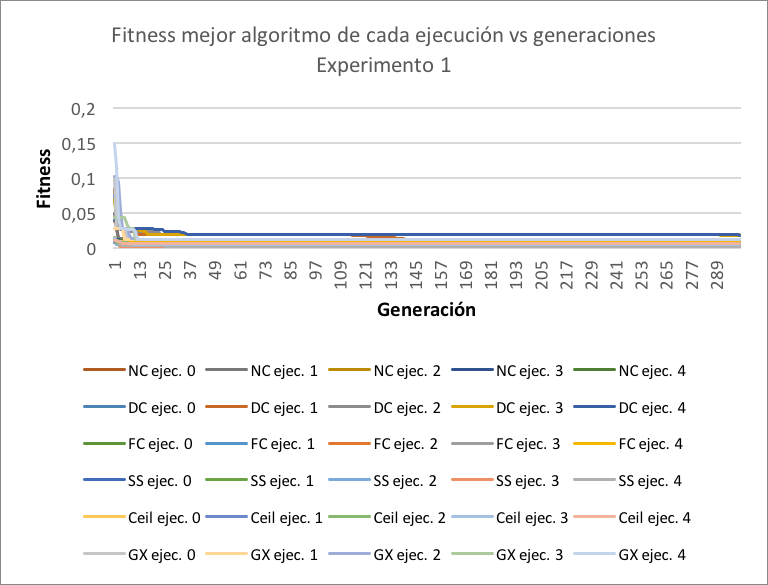
\includegraphics[width=13cm]{images/cap6/convergencia_exp1.png}
    \captionof{figure}{Fitness por generación experimento 1 (Elaboración propia, 2015)}\label{fig:convergencia_exp1}
\endgroup

\begingroup
    \centering
    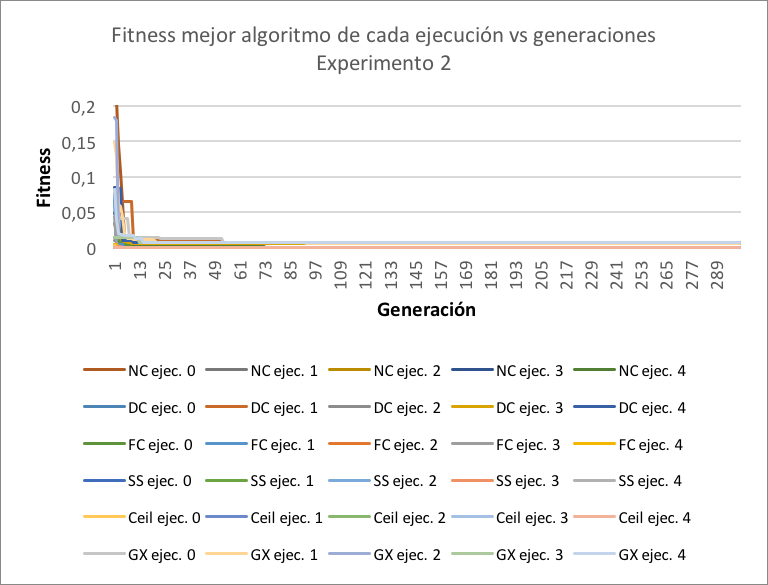
\includegraphics[width=13cm]{images/cap6/convergencia_exp2.png}
    \captionof{figure}{Fitness por generación experimento 2 (Elaboración propia, 2015)}\label{fig:convergencia_exp2}
\endgroup

Existe variedad en relación a la calidad de los algoritmos obtenidos. La distribución de los algoritmos por medio de su calidad en el proceso evolutivo a través de las generaciones es presentada en las Figuras \ref{fig:box_whisker_exp1} y \ref{fig:box_whisker_exp2}. En la Figura \ref{fig:box_whisker_exp1} se presenta el \textit{fitness} de los algoritmos obtenidos en el proceso evolutivo del experimento 1 y ejecución 0 que utiliza el grupo de evolución $SS$ ($ANKPSS1$) y el experimento 2 con ejecución 0 que utiliza el mismo grupo de evolución ($AIKPSS1$), mediante el uso de un gráfico de Box and Whisker. En estas Figuras solo son representadas algunas generaciones ($0, 25, 50, 75, …, 299$), para así poder apreciar la distribución de los algoritmos, debido a su extensa cantidad. Para cada una de las generaciones se presenta una división en cuatro secciones que representan a cada uno de los cuartiles y algunos \textit{outliers}. Cada uno de los cuartiles representa un 25\% (cuartil 1 25\%, cuartil 2 50\%, etc) de los individuos de cada generación. Dentro de las generaciones, aparece una $x$ que representa el promedio de los individuos de la generación, y una línea que divide la “caja” representando la media de los datos. De esta distribución, es posible inferir que el proceso evolutivo, al inicio la mayor cantidad de los individuos posee los peores valores de \textit{fitness}, donde los cuatro cuartiles se encuentran en un rango de $0,6$ a $1,2$ para el experimento 1 y $0,8$ a $1,0$ para el experimento 2, y a medida que avanzan las generaciones, esta distribución tiende a mejores valores. En general, es posible apreciar que existen varios \textit{outliers} en ambos gráficos, los que se encuentran distribuidos en la parte superior de las “cajas”. Esto se debe principalmente a que en cada generación aparecen nuevos individuos auto generados para completar la población, luego de aplicar el proceso de variación (mutación, cruzamiento, reproducción, etc). En ambos gráficos el \textit{fitness} promedio converge a valores menores a $0,2$, mientras que la media tiende a $0$ o valores muy pequeños. De esto último se desprende que al avanzar las generaciones, la mayoría de los individuos, sobre el 50\%, obtienen buenos resultados (menores a $0,1$). La distribución de los demás algoritmos generados por los otros experimentos es similar y puede ser inferida de la Tabla \ref{tab:resumen_exp1} y Tabla \ref{tab:resumen_exp2} donde se muestra el resumen de los experimentos 1 y 2, con sus respectivos sub-experimentos. En estas tablas se muestran datos generales de todos algoritmos obtenidos en la ejecución del sub-experimento para cada uno de los experimentos relacionados al PM-01, por ejemplo “NC ejec. 0” es la ejecución 0 del sub-experimento que utiliza el grupo NC. Dada la gran cantidad de algoritmos generados por sub-experimento y más aún los obtenidos de ambos experimentos durante el proceso evolutivo (aproximadamente 150 mil por sub-experimento), es que se selecciona al mejor de cada ejecución para ser evaluado con las instancias de prueba. Esto resulta en la evaluación de 60 algoritmos, siendo cinco los extraídos de cada uno de los 12 experimentos (experimento 1a, experimento 2a, experimento 1b, experimento 2b, etc). Los algoritmos a evaluar son los propuestos en la Tabla \ref{tab:mejores_pm01_exp1} y Tabla \ref{tab:mejores_pm01_exp2} para los experimentos 1 y 2 respectivamente. En las tablas donde se presentan los mejores algoritmos, el nombre que éstos tienen posee la siguiente forma: Algoritmo - Experimento (Tradicional \textbf{(N)} o co-evolución utilizando método de islas \textbf{(I)}) - Problema - Grupo instancias - Correlativo de 1 a 5. Un ejemplo de esto último es ANKPNC1, que se lee como Algoritmo (A) del experimento tradicional (N) para el problema de la mochila (KP) utilizando el grupo de instancias NC (NC) obtenido en la ejecución 1.

\begingroup
    \centering
    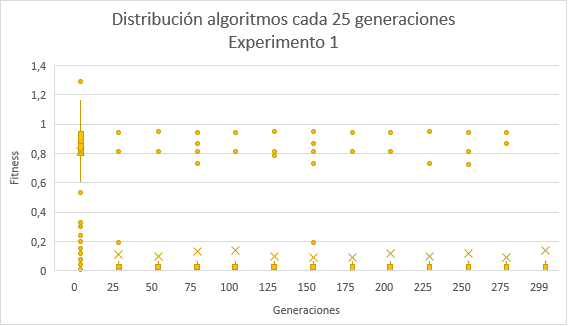
\includegraphics[width=13cm]{images/cap6/box_whisker_exp1.png}
    \captionof{figure}{Distribución algoritmos experimento 1 (Elaboración propia, 2015)}\label{fig:box_whisker_exp1}
\endgroup

\begingroup
    \centering
    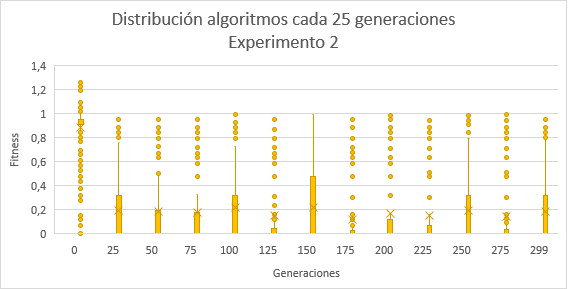
\includegraphics[width=13cm]{images/cap6/box_whisker_exp2.png}
    \captionof{figure}{Distribución algoritmos experimento 2 (Elaboración propia, 2015)}\label{fig:box_whisker_exp2}
\endgroup

\begin{table}[hbtp!]
\caption{Datos generales de los algoritmos obtenidos en el experimento 1}\label{tab:resumen_exp1}
\small
\centering
\begin{center}
\rowcolors{2}{gray!25}{white}
\begin{tabular}{c|ccc|ccc|ccc}
\hline
{\textbf{}} & \multicolumn{3}{c}{{\textbf{Fitness}}} & \multicolumn{3}{c}{{\textbf{Nº Nodos}}} & \multicolumn{3}{c}{{\textbf{Altura}}} \\ \hline
{\textbf{Nombre}} & \textbf{Peor} &	\textbf{Prom.} & \textbf{Mejor} & \textbf{Min.} & \textbf{Prom.} & \textbf{Máximo} & \textbf{Min.} & \textbf{Prom.} & \textbf{Máximo} \\ \hline
NC ejec. 0 & 1,1688 & 0,2232 & 0,0038 & 2 & 13,08 & 122 & 2 & 5,27 & 10 \\
NC ejec. 1 & 1,2133 & 0,2827 & 0,0037 & 2 & 12,16 & 116 & 2 & 4,70 & 10 \\
NC ejec. 2 & 1,3316 & 0,2309 & 0,0039 & 2 & 12,13 & 133 & 2 & 5,89 & 10 \\
NC ejec. 3 & 1,1607 & 0,2365 & 0,0057 & 2 & 10,59 & 121 & 2 & 4,38 & 10 \\
NC ejec. 4 & 1,2449 & 0,1393 & 0,0047 & 2 & 10,48 & 138 & 2 & 4,45 & 10 \\ \hline
DC ejec. 0 & 1,1567 & 0,2557 & 0,0178 & 2 & 12,52 & 109 & 2 & 5,78 & 10 \\
DC ejec. 1 & 1,1516 & 0,2262 & 0,0118 & 2 & 12,89 & 139 & 2 & 5,23 & 10 \\
DC ejec. 2 & 1,3174 & 0,2372 & 0,0187 & 2 & 12,39 & 126 & 2 & 4,60 & 10 \\
DC ejec. 3 & 1,2252 & 0,2168 & 0,0176 & 2 & 11,65 & 109 & 2 & 5,01 & 10 \\
DC ejec. 4 & 1,1508 & 0,2276 & 0,0178 & 2 & 10,81 & 144 & 2 & 5,40 & 10 \\ \hline
FC ejec. 0 & 1,1567 & 0,1775 & 0,0093 & 2 & 11,49 & 98 & 2 & 4,18 & 10 \\
FC ejec. 1 & 1,2166 & 0,1215 & 0,0096 & 2 & 6,54 & 105 & 2 & 3,56 & 10 \\
FC ejec. 2 & 1,2905 & 0,1699 & 0,0080 & 2 & 11,44 & 124 & 2 & 4,25 & 10 \\
FC ejec. 3 & 1,2133 & 0,2404 & 0,0078 & 2 & 9,47 & 103 & 2 & 4,93 & 10 \\
FC ejec. 4 & 1,2000 & 0,1936 & 0,0096 & 2 & 7,04 & 106 & 2 & 3,25 & 10 \\ \hline
SS ejec. 0 & 1,2900 & 0,1289 & 0,0021 & 2 & 10,85 & 123 & 2 & 3,96 & 10 \\
SS ejec. 1 & 1,3033 & 0,0420 & 0,0021 & 2 & 11,00 & 121 & 2 & 4,42 & 10 \\
SS ejec. 2 & 1,2389 & 0,2545 & 0,0021 & 2 & 11,27 & 108 & 2 & 4,76 & 10 \\
SS ejec. 3 & 1,2067 & 0,1964 & 0,0022 & 2 & 8,50 & 131 & 2 & 4,36 & 10 \\
SS ejec. 4 & 1,2493 & 0,1792 & 0,0021 & 2 & 10,42 & 125 & 2 & 5,43 & 10 \\ \hline
Ceil ejec. 0 & 1,2383 & 0,2175 & 0,0051 & 2 & 12,36 & 132 & 2 & 4,24 & 10 \\
Ceil ejec. 1 & 1,1510 & 0,1895 & 0,0058 & 2 & 11,05 & 117 & 2 & 5,35 & 10 \\
Ceil ejec. 2 & 1,2293 & 0,1332 & 0,0048 & 2 & 12,75 & 136 & 2 & 5,88 & 10 \\
Ceil ejec. 3 & 1,2128 & 0,1866 & 0,0048 & 2 & 10,51 & 134 & 2 & 4,26 & 10 \\
Ceil ejec. 4 & 1,2338 & 0,2189 & 0,0057 & 2 & 8,65 & 124 & 2 & 4,38 & 10 \\ \hline
GX ejec. 0 & 1,2172 & 0,2187 & 0,0126 & 2 & 8,86 & 120 & 2 & 4,60 & 10 \\
GX ejec. 1 & 1,1209 & 0,1530 & 0,0126 & 2 & 10,56 & 102 & 2 & 4,53 & 10 \\
GX ejec. 2 & 1,3110 & 0,2769 & 0,0123 & 2 & 12,16 & 139 & 2 & 4,68 & 10 \\
GX ejec. 3 & 1,1931 & 0,2250 & 0,0126 & 2 & 8,40 & 115 & 2 & 4,36 & 10 \\
GX ejec. 4 & 1,1819 & 0,2192 & 0,0126 & 2 & 9,37 & 123 & 2 & 4,43 & 10 \\
\hline
\end{tabular}
\end{center}
\caption*{(Elaboración propia, 2015)}
\end{table}

\begin{table}[hbtp!]
\caption{Datos generales de los algoritmos obtenidos en el experimento 2}\label{tab:resumen_exp2}
\small
\centering
\begin{center}
\rowcolors{2}{gray!25}{white}
\begin{tabular}{c|ccc|ccc|ccc}
\hline
{\textbf{}} & \multicolumn{3}{c}{{\textbf{Fitness}}} & \multicolumn{3}{c}{{\textbf{Nº Nodos}}} & \multicolumn{3}{c}{{\textbf{Altura}}} \\ \hline
{\textbf{Nombre}} & \textbf{Peor} &	\textbf{Prom.} & \textbf{Mejor} & \textbf{Min.} & \textbf{Prom.} & \textbf{Máximo} & \textbf{Min.} & \textbf{Prom.} & \textbf{Máximo} \\ \hline
NC ejec. 0 & 1,2700 & 0,2838 & 0,0000 & 2 & 9,67 & 120 & 2 & 4,89 & 10 \\
NC ejec. 1 & 1,3033 & 0,3810 & 0,0000 & 2 & 10,50 & 163 & 2 & 4,96 & 10 \\
NC ejec. 2 & 1,3233 & 0,3724 & 0,0000 & 2 & 10,42 & 127 & 2 & 4,28 & 10 \\
NC ejec. 3 & 1,3200 & 0,3549 & 0,0000 & 2 & 10,29 & 129 & 2 & 5,00 & 10 \\
NC ejec. 4 & 1,3000 & 0,3109 & 0,0000 & 2 & 7,67 & 133 & 2 & 4,06 & 10 \\ \hline
DC ejec. 0 & 1,2033 & 0,4185 & 0,0057 & 2 & 9,07 & 96 & 2 & 4,22 & 10 \\
DC ejec. 1 & 1,2967 & 0,3334 & 0,0057 & 2 & 9,97 & 119 & 2 & 4,15 & 10 \\
DC ejec. 2 & 1,2700 & 0,4415 & 0,0056 & 2 & 12,35 & 120 & 2 & 4,13 & 10 \\
DC ejec. 3 & 1,2667 & 0,3839 & 0,0057 & 2 & 9,74 & 110 & 2 & 4,63 & 10 \\
DC ejec. 4 & 1,2700 & 0,3774 & 0,0069 & 2 & 9,34 & 111 & 2 & 3,73 & 10 \\ \hline
FC ejec. 0 & 1,3733 & 0,3392 & 0,0000 & 2 & 8,27 & 142 & 2 & 4,08 & 10 \\
FC ejec. 1 & 1,2733 & 0,3799 & 0,0000 & 2 & 7,35 & 138 & 2 & 3,96 & 10 \\
FC ejec. 2 & 1,2803 & 0,3511 & 0,0000 & 2 & 8,94 & 140 & 2 & 4,23 & 10 \\
FC ejec. 3 & 1,2333 & 0,3418 & 0,0000 & 2 & 7,26 & 112 & 2 & 3,70 & 10 \\
FC ejec. 4 & 1,2267 & 0,2614 & 0,0000 & 2 & 6,31 & 100 & 2 & 3,51 & 10 \\ \hline
SS ejec. 0 & 1,2600 & 0,1862 & 0,0000 & 2 & 11,24 & 108 & 2 & 4,86 & 10 \\
SS ejec. 1 & 1,2267 & 0,2571 & 0,0000 & 2 & 9,27 & 98 & 2 & 4,15 & 10 \\
SS ejec. 2 & 1,3100 & 0,2828 & 0,0000 & 2 & 10,86 & 123 & 2 & 3,95 & 10 \\
SS ejec. 3 & 1,1867 & 0,2619 & 0,0000 & 2 & 10,96 & 130 & 2 & 4,78 & 10 \\
SS ejec. 4 & 1,3167 & 0,2163 & 0,0000 & 2 & 10,85 & 125 & 2 & 4,46 & 10 \\ \hline
Ceil ejec. 0 & 1,2267 & 0,2381 & 0,0000 & 2 & 9,14 & 107 & 2 & 4,32 & 10 \\
Ceil ejec. 1 & 1,2400 & 0,2326 & 0,0000 & 2 & 9,37 & 119 & 2 & 4,65 & 10 \\
Ceil ejec. 2 & 1,2733 & 0,1516 & 0,0000 & 2 & 9,38 & 118 & 2 & 4,27 & 10 \\
Ceil ejec. 3 & 1,3067 & 0,2221 & 0,0000 & 2 & 9,84 & 122 & 2 & 4,36 & 10 \\
Ceil ejec. 4 & 1,2408 & 0,2770 & 0,0000 & 2 & 9,42 & 115 & 2 & 4,35 & 10 \\ \hline
GX ejec. 0 & 1,2900 & 0,3662 & 0,0075 & 2 & 9,27 & 120 & 2 & 4,35 & 10 \\
GX ejec. 1 & 1,2567 & 0,3916 & 0,0064 & 2 & 11,46 & 133 & 2 & 4,61 & 10 \\
GX ejec. 2 & 1,2667 & 0,3458 & 0,0077 & 2 & 10,79 & 110 & 2 & 4,63 & 10 \\
GX ejec. 3 & 1,2932 & 0,3675 & 0,0075 & 2 & 9,65 & 123 & 2 & 4,67 & 10 \\
GX ejec. 4 & 1,2933 & 0,3994 & 0,0076 & 2 & 10,44 & 122 & 2 & 5,17 & 10 \\
\hline
\end{tabular}
\end{center}
\caption*{(Elaboración propia, 2015)}
\end{table}

En relación al \textit{fitness}, no existe una gran variación en la calidad de la GAA para los distintos algoritmos obtenidos durante el proceso evolutivo para el mismo conjunto de instancias. En las tablas \ref{tab:resumen_exp1} y \ref{tab:resumen_exp2} aparecen datos del mejor, peor y promedio del \textit{fitness} de todos los algoritmos generados utilizando alguno de los grupos de instancias clasificados en el sub-capítulo \ref{cap:sel_casos_adapt_pm01}. En relación a la Tabla \ref{tab:resumen_exp1}, es posible apreciar que el resultado tanto del mejor, peor y el promedio del \textit{fitness} de los algoritmos tiende a valores similares, lo que complementa las consideraciones mencionadas en \ref{cap:consideraciones}. En relación a los resultados del \textit{fitness} obtenido entre los distintos grupos de instancias, es posible apreciar que en algunos casos, existe una mayor diferencia que la presentada en los resultados dentro del mismo grupo, lo que se debe principalmente a las características del grupo de instancias utilizado en el proceso evolutivo. Para la Tabla \ref{tab:resumen_exp2} se ve que ocurre un efecto similar, tanto en la relación entre los algoritmos del mismo grupo, como en la comparación con los de otros grupos. Finalmente, los resultados que se obtienen en cada uno de los grupos al ser comparados entre experimentos, presentan una variación en la que los algoritmos del experimento 1 obtienen mejores resultados. Esta variación ocurre por que en el experimento 2 se generan algoritmos en distintas poblaciones con distintos criterios de evaluación (islas), lo que conlleva a una mayor variabilidad que la presentada en el experimento 1.

La variación de los algoritmos obtenidos en la GAA está relacionada con la estructura  que posee el árbol sintáctico obtenido durante el proceso evolutivo. En las tablas \ref{tab:resumen_exp1} y \ref{tab:resumen_exp2} aparecen datos del máximo, mínimo y promedio del número de nodos y la altura. Con respecto al número de nodos, existe variación en los algoritmos del mismo grupo y al ser comparados entre los distintos grupos. Aunque el número máximo de nodos alcanza valores sobre 100, el promedio es siempre menor a 15, cuyo valor fue determinado como máximo para no interferir en la calidad de los algoritmos (factor de legibilidad, véase \ref{cap:func_eval_pm01}). En relación a la altura de los árboles que representan a los algoritmos, se ve que también existe variación tanto entre los grupos como al compararlos con otros. El promedio de éstos tiende a valores entre 3 y 5, lo que se relaciona directamente con el número máximo permitido de nodos, ya que algunos de estos nodos representan funciones, las que solo tienen permitido un número determinado de hijos.

La calidad de los algoritmos obtenidos mediante el proceso evolutivo no tiene relación con el tiempo que demora el proceso evolutivo ni la generación en la que el o los mejores algoritmos aparecen dentro de la ejecución de este proceso. En las tablas \ref{tab:mejores_pm01_exp1} y \ref{tab:mejores_pm01_exp2}, es posible apreciar el tiempo de evolución de cada una de las ejecuciones y la generación en la que aparece el mejor individuo de ésta. En estas tablas es posible notar que existe variación tanto en el tiempo de cada una de las ejecuciones del proceso evolutivo y en la generación en la que el mejor individuo aparece.

El tamaño de los árboles que componen los algoritmos obedece al rango de tamaño predefinido en la función de legibilidad que se encuentra dentro de la función de evaluación (\textit{fitness}). En la Tabla \ref{tab:mejores_pm01_exp1} y \ref{tab:mejores_pm01_exp2} se muestra que no existe una convergencia hacia árboles de similares dimensiones. Como se observa en estas tablas, los árboles seleccionados varían entre 3 y 15 nodos con una altura entre 2 y 7 para el experimento 1, y entre 3 y 15 nodos, con una altura entre 2 y 6 para el experimento 2.

\begin{table}[hbtp!]
\caption{Datos generales del mejor algoritmo de cada experimento del experimento 1}\label{tab:mejores_pm01_exp1}
\small
\centering
\begin{center}
\rowcolors{2}{gray!25}{white}
\begin{tabular}{cccccc}
{\textbf{{Nombre}}} & {\textbf{{Fitness}}} & {\textbf{\begin{tabular}[c]{@{}c@{}}Nº de \\nodos\end{tabular}}} & {\textbf{{Altura}}} & {\textbf{\begin{tabular}[c]{@{}c@{}}Ejecución en la \\que aparece\end{tabular}}} & {\textbf{\begin{tabular}[c]{@{}c@{}}Tiempo \\(min)\end{tabular}}}\\ \hline
ANKPNC1 & 0,0038 & 15 & 6 & 30 & 21,10 \\
ANKPNC2 & 0,0037 & 15 & 5 & 231 & 23,09 \\
ANKPNC3 & 0,0039 & 14 & 7 & 100 & 24,40 \\
ANKPNC4 & 0,0057 & 15 & 5 & 14 & 19,25 \\
ANKPNC5 & 0,0047 & 9 & 4 & 17 & 18,58 \\ \hline
ANKPDC1 & 0,0187 & 14 & 6 & 291 & 17,16 \\
ANKPDC2 & 0,0118 & 15 & 6 & 138 & 30,04 \\
ANKPDC3 & 0,0187 & 15 & 5 & 57 & 19,65 \\
ANKPDC4 & 0,0187 & 13 & 5 & 16 & 17,30 \\
ANKPDC5 & 0,0187 & 15 & 7 & 148 & 19,49 \\ \hline
ANKPFC1 & 0,0093 & 14 & 4 & 4 & 17,63 \\
ANKPFC2 & 0,0096 & 3 & 2 & 0 & 22,49 \\
ANKPFC3 & 0,0082 & 14 & 5 & 129 & 22,33 \\
ANKPFC4 & 0,0078 & 15 & 8 & 282 & 24,55 \\
ANKPFC5 & 0,0096 & 3 & 2 & 0 & 19,92 \\ \hline
ANKPSS1 & 0,0021 & 14 & 4 & 4 & 13,65 \\
ANKPSS2 & 0,0021 & 10 & 4 & 3 & 19,70 \\
ANKPSS3 & 0,0021 & 15 & 5 & 94 & 20,74 \\
ANKPSS4 & 0,0022 & 5 & 3 & 3 & 18,90 \\
ANKPSS5 & 0,0021 & 9 & 5 & 32 & 16,88 \\ \hline
ANKPCeil1 & 0,0051 & 13 & 4 & 23 & 10,15 \\
ANKPCeil2 & 0,0058 & 13 & 5 & 12 & 10,96 \\
ANKPCeil3 & 0,0049 & 15 & 7 & 95 & 14,78 \\
ANKPCeil4 & 0,0048 & 11 & 4 & 8 & 11,63 \\
ANKPCeil5 & 0,0068 & 5 & 3 & 36 & 12,61 \\ \hline
ANKPGX1 & 0,0167 & 8 & 5 & 8 & 13,45 \\
ANKPGX2 & 0,0073 & 8 & 5 & 5 & 11,66 \\
ANKPGX3 & 0,0164 & 9 & 4 & 46 & 13,23 \\
ANKPGX4 & 0,0077 & 9 & 4 & 10 & 14,42 \\
ANKPGX5 & 0,0142 & 15 & 5 & 11 & 12,46 \\
\hline
\end{tabular}
\end{center}
\caption*{(Elaboración propia, 2015)}
\end{table}

\begin{table}[hbtp!]
\caption{Datos generales del mejor algoritmo de cada experimento del experimento 2}\label{tab:mejores_pm01_exp2}
\small
\centering
\begin{center}
\rowcolors{2}{gray!25}{white}
\begin{tabular}{ccccccc}
{\textbf{{Nombre}}} & {\textbf{{Fitness}}} & {\textbf{\begin{tabular}[c]{@{}c@{}}Nº de \\nodos\end{tabular}}} & {\textbf{{Altura}}} & {\textbf{\begin{tabular}[c]{@{}c@{}}Ejecución en la \\que aparece\end{tabular}}} & {\textbf{\begin{tabular}[c]{@{}c@{}}Isla en la \\que aparece\end{tabular}}} & {\textbf{\begin{tabular}[c]{@{}c@{}}Tiempo \\(min)\end{tabular}}}\\ \hline
AIKPNC1 & 0,0048 & 13 & 6 & 2 & 23 & 22,66 \\
AIKPNC2 & 0,0047 & 11 & 5 & 2 & 112 & 26,93 \\
AIKPNC3 & 0,0056 & 14 & 4 & 2 & 42 & 21,01 \\
AIKPNC4 & 0,0057 & 9 & 4 & 1 & 39 & 23,82 \\
AIKPNC5 & 0,0057 & 5 & 3 & 1 y 3 & 62 y 62 & 21,94 \\ \hline
AIKPDC1 & 0,0187 & 13 & 5 & 1 & 67 & 18,22 \\
AIKPDC2 & 0,0173 & 15 & 6 & 2 & 277 & 22,52 \\
AIKPDC3 & 0,0163 & 15 & 4 & 1 & 90 & 17,74 \\
AIKPDC4 & 0,0187 & 12 & 5 & 1 & 19 & 20,73 \\
AIKPDC5 & 0,0271 & 10 & 3 & 0 & 4 & 18,63 \\ \hline
AIKPFC1 & 0,0096 & 6 & 3 & 0 y 2 & 0 y 2 & 18,17 \\
AIKPFC2 & 0,0096 & 3 & 2 & 0 & 3 & 19,27 \\
AIKPFC3 & 0,0084 & 15 & 6 & 2 & 227 & 18,96 \\
AIKPFC4 & 0,0096 & 3 & 2 & 0, 1 y 3 & 2, 0 y 2 & 18,68 \\
AIKPFC5 & 0,0096 & 3 & 2 & 0 & 0 & 21,90 \\ \hline
AIKPSS1 & 0,0021 & 15 & 5 & 2 & 124 & 18,62 \\
AIKPSS2 & 0,0096 & 14 & 6 & 0 & 42 & 17,52 \\
AIKPSS3 & 0,0084 & 13 & 4 & 0 & 7 & 17,74 \\
AIKPSS4 & 0,0096 & 11 & 5 & 0 & 12 & 19,04 \\
AIKPSS5 & 0,0096 & 15 & 6 & 2 & 32 & 19,19 \\ \hline
AIKPCeil1 & 0,0057 & 10 & 4 & 2 & 62 y 62 & 17,85 \\
AIKPCeil2 & 0,0068 & 7 & 3 & 0 y 2 & 2 y 0 & 19,34 \\
AIKPCeil3 & 0,0058 & 15 & 6 & 2 & 60 & 20,64 \\
AIKPCeil4 & 0,0057 & 10 & 4 & 2 & 25 & 17,58 \\
AIKPCeil5 & 0,0075 & 14 & 6 & 0 & 145 & 24,74 \\ \hline
AIKPGX1 & 0,0157 & 11 & 5 & 2 & 241 & 19,48 \\
AIKPGX2 & 0,0063 & 11 & 5 & 0 y 2 & 214 y 222 & 15,25 \\
AIKPGX3 & 0,0150 & 15 & 5 & 0 y 2 & 22 y 11 & 18,46 \\
AIKPGX4 & 0,0077 & 15 & 5 & 0 & 12 & 16,77 \\
AIKPGX5 & 0,0147 & 9 & 4 & 2 & 34 & 16,94 \\
\hline
\end{tabular}
\end{center}
\caption*{(Elaboración propia, 2015)}
\end{table}

Los algoritmos generados son mejores para instancias de mayor tamaño. En el diseño del experimento, el criterio de división de las instancias para las islas del experimento 2 fue por medio del tamaño de éstas, siendo el tamaño la cantidad de ítems que posee la instancia y no la escala en que los valores del peso y beneficio se encuentren. En la Tabla \ref{tab:mejores_islas_pm01} se presentan los resultados de los mejores algoritmos de cada isla por ejecución. La isla 0 se compone de una función de evaluación por HITS y los grupos de instancias de tamaño 50 y 100. La isla 1 se compone de una función de evaluación por ERP y los grupos de instancias de tamaño 200 y 500, la isla 2 se compone de una función de evaluación por ERP y los grupos de instancias de tamaño 50 y 100, y finalmente, la isla 3 se compone de una función de evaluación por HITS y los grupos de instancias de tamaño 200 y 500. En esta Tabla se puede ver los resultados del ERP que obtuvo cada uno de éstos y el \textit{fitness} con el que finalmente fueron evaluados durante el proceso evolutivo. Los algoritmos generados en las islas 1 y 3 presentan un menor ERP en comparación a los generados en las islas 0 y 2. La Tabla \ref{tab:resumen_mejores_islas_pm01} presenta un resumen de la Tabla \ref{tab:mejores_islas_pm01} donde es más fácil apreciar la comparación entre las distintas islas. Considerando los resultados obtenidos en las ejecuciones de los diversos experimentos que utilizan gran variedad de grupos de instancias, es posible concluir que los mejores resultados en el proceso evolutivo son obtenidos por las instancias de mayor tamaño. Por otra parte, los resultados para las islas 0 y 3, presentan una gran variación entre el ERP y el \textit{fitness}, mientras que en las islas 1 y 2, los resultados son similares. Esto se debe a la particularidad de cada una de las funciones de evaluación, que buscan medir con un criterio distinto la calidad de los algoritmos generados. De lo anterior se desprende en relación al tamaño que es recomendable el uso de instancias de mayor tamaño para el proceso evolutivo. Mientras tanto, en relación al uso de la función de evaluación, cuando ésta sea relacionada a los HITS (cantidad de soluciones óptimas obtenidas) se sugiere la incorporación un porcentaje menor que considere el ER, esto debido a que la selección de los algoritmos es realizada considerando el valor del \textit{fitness} que considera solo a los algoritmos que obtienen un ER menor al \% determinado, por lo que un algoritmo que obtiene un ERP un poco mayor al aceptado por la función de evaluación HITS es penalizado de la misma forma que un algoritmo que obtenga un resultado muy malo. Por ejemplo, si el ER máximo para considerar un \textit{hit} es de $1,0\%$, un algoritmo que obtenga un $1,1\%$ de ER tiene el mismo \textit{fitness} que un algoritmo con un ER de $100\%$.

\begin{table}[hbtp!]
\caption{Resultados del ERP y fitness para el mejor individuo de cada isla de los sub-experimentos del experimento 2}\label{tab:mejores_islas_pm01}
\small
\centering
\begin{center}
\rowcolors{2}{gray!25}{white}
\begin{tabular}{c|cc|cc|cc|cc}
{\textbf{}} & \multicolumn{2}{c|}{{\textbf{Isla 0}}} & \multicolumn{2}{c|}{{\textbf{Isla 1}}} & \multicolumn{2}{c|}{{\textbf{Isla 2}}} & \multicolumn{2}{c}{{\textbf{Isla 3}}}\\ \hline
{\textbf{Nombre}} & {\textbf{ERP}} & {\textbf{Fitness}} & {\textbf{ERP}} & {\textbf{Fitness}} & {\textbf{ERP}} & {\textbf{Fitness}} & {\textbf{ERP}} & {\textbf{Fitness}} \\ \hline
NC ejec. 0 & 0.0070 & 0.1583 & 0.0029 & 0.0028 & 0.0068 & 0.0065 & 0.0029 & 0.0000 \\
NC ejec. 1 & 0.0070 & 0.1583 & 0.0029 & 0.0028 & 0.0070 & 0.0066 & 0.0029 & 0.0000 \\
NC ejec. 2 & 0.0055 & 0.0000 & 0.0029 & 0.0028 & 0.0053 & 0.0050 & 0.0029 & 0.0000 \\
NC ejec. 3 & 0.0053 & 0.0000 & 0.0029 & 0.0028 & 0.0053 & 0.0050 & 0.0033 & 0.0000 \\
NC ejec. 4 & 0.0092 & 0.3167 & 0.0029 & 0.0028 & 0.0090 & 0.0086 & 0.0029 & 0.0000 \\ \hline
DC ejec. 0 & 0.0497 & 0.4750 & 0.0060 & 0.0057 & 0.0333 & 0.0316 & 0.0060 & 0.3167 \\
DC ejec. 1 & 0.0497 & 0.4750 & 0.0060 & 0.0057 & 0.0281 & 0.0267 & 0.0104 & 0.3167 \\
DC ejec. 2 & 0.0497 & 0.4750 & 0.0059 & 0.0056 & 0.0279 & 0.0265 & 0.0168 & 0.1583 \\
DC ejec. 3 & 0.0497 & 0.4750 & 0.0060 & 0.0057 & 0.0318 & 0.0302 & 0.0069 & 0.3167 \\
DC ejec. 4 & 0.0497 & 0.4750 & 0.0073 & 0.0069 & 0.0497 & 0.0472 & 0.0074 & 0.3167 \\ \hline
FC ejec. 0 & 0.0151 & 0.6333 & 0.0036 & 0.0034 & 0.0151 & 0.0143 & 0.0051 & 0.0000 \\
FC ejec. 1 & 0.0151 & 0.6333 & 0.0051 & 0.0049 & 0.0151 & 0.0143 & 0.0051 & 0.0000 \\
FC ejec. 2 & 0.0135 & 0.4817 & 0.0046 & 0.0044 & 0.0128 & 0.0122 & 0.0051 & 0.0000 \\
FC ejec. 3 & 0.0151 & 0.6333 & 0.0051 & 0.0049 & 0.0151 & 0.0143 & 0.0051 & 0.0000 \\
FC ejec. 4 & 0.0151 & 0.6333 & 0.0051 & 0.0049 & 0.0151 & 0.0143 & 0.0051 & 0.0000 \\ \hline
SS ejec. 0 & 0.0027 & 0.0000 & 0.0004 & 0.0004 & 0.0027 & 0.0025 & 0.0003 & 0.0000 \\
SS ejec. 1 & 0.0036 & 0.0000 & 0.0003 & 0.0003 & 0.0036 & 0.0035 & 0.0031 & 0.0000 \\
SS ejec. 2 & 0.0033 & 0.0000 & 0.0004 & 0.0003 & 0.0033 & 0.0032 & 0.0027 & 0.0000 \\
SS ejec. 3 & 0.0063 & 0.0000 & 0.0003 & 0.0003 & 0.0035 & 0.0033 & 0.0027 & 0.0000 \\
SS ejec. 4 & 0.0036 & 0.0000 & 0.0003 & 0.0003 & 0.0036 & 0.0035 & 0.0015 & 0.0000 \\ \hline
Ceil ejec. 0 & 0.0074 & 0.0000 & 0.0004 & 0.0004 & 0.0066 & 0.0063 & 0.0011 & 0.0000 \\
Ceil ejec. 1 & 0.0091 & 0.1583 & 0.0004 & 0.0004 & 0.0091 & 0.0087 & 0.0011 & 0.0000 \\
Ceil ejec. 2 & 0.0076 & 0.0000 & 0.0004 & 0.0004 & 0.0075 & 0.0071 & 0.0043 & 0.0000 \\
Ceil ejec. 3 & 0.0069 & 0.0000 & 0.0005 & 0.0005 & 0.0068 & 0.0065 & 0.0053 & 0.0000 \\
Ceil ejec. 4 & 0.0100 & 0.1583 & 0.0025 & 0.0024 & 0.0100 & 0.0095 & 0.0051 & 0.0000 \\ \hline
GX ejec. 0 & 0.0179 & 0.5700 & 0.0079 & 0.0075 & 0.0166 & 0.0157 & 0.0085 & 0.1900 \\
GX ejec. 1 & 0.0160 & 0.3800 & 0.0067 & 0.0064 & 0.0160 & 0.0152 & 0.0085 & 0.1900 \\
GX ejec. 2 & 0.0179 & 0.5700 & 0.0081 & 0.0077 & 0.0179 & 0.0170 & 0.0085 & 0.1900 \\
GX ejec. 3 & 0.0179 & 0.5700 & 0.0079 & 0.0075 & 0.0179 & 0.0170 & 0.0085 & 0.1900 \\
GX ejec. 4 & 0.0179 & 0.5700 & 0.0080 & 0.0076 & 0.0177 & 0.0168 & 0.0085 & 0.1900 \\
\hline
\end{tabular}
\end{center}
\caption*{(Elaboración propia, 2015)}
\end{table}

\begin{table}[hbtp!]
\caption{Resumen por isla de cada sub-experimento del experimento 2}\label{tab:resumen_mejores_islas_pm01}
\small
\centering
\begin{center}
\rowcolors{2}{gray!25}{white}
\begin{tabular}{c|ccc|ccc}
{\textbf{}} & \multicolumn{3}{c|}{{\textbf{ERP}}} & \multicolumn{3}{c}{{\textbf{Fitness}}} \\ \hline
{\textbf{Nombre Isla}} & {\textbf{Peor}} & {\textbf{Prom.}} & {\textbf{Mejor}} & {\textbf{Peor}} & {\textbf{Prom.}} & {\textbf{Mejor}}\\ \hline
Isla 0 & 0,0497 & 0,0168 & 0,0027 & 0,6333 & 0,3000 & 0,0000 \\
Isla 1 & 0,0081 & 0,0038 & 0,0003 & 0,0077 & 0,0036 & 0,0003 \\
Isla 2 & 0,0497 & 0,0140 & 0,0027 & 0,0472 & 0,0133 & 0,0025 \\
Isla 3 & 0,0168 & 0,0053 & 0,0003 & 0,3167 & 0,0792 & 0,0000 \\
\hline
\end{tabular}
\end{center}
\caption*{(Elaboración propia, 2015)}
\end{table}

\subsection{Resultados de la evaluación}

Los algoritmos seleccionados para el proceso de evaluación empeoran al comparar los resultados obtenidos para los grupos de instancias de evolución en comparación a los de evaluación. La Figura \ref{fig:evol_vs_eval_exp1} muestra los resultados de la comparación entre los resultados de la evolución y evaluación para el experimento 1. En ésta es posible apreciar que los resultados de la evaluación empeoran para todos los sub-experimentos correspondientes al experimento 1. La Figura \ref{fig:evol_vs_eval_exp2} muestra los resultados de la comparación para el experimento 2, donde se ve que ocurre un efecto similar.

\begingroup
    \centering
    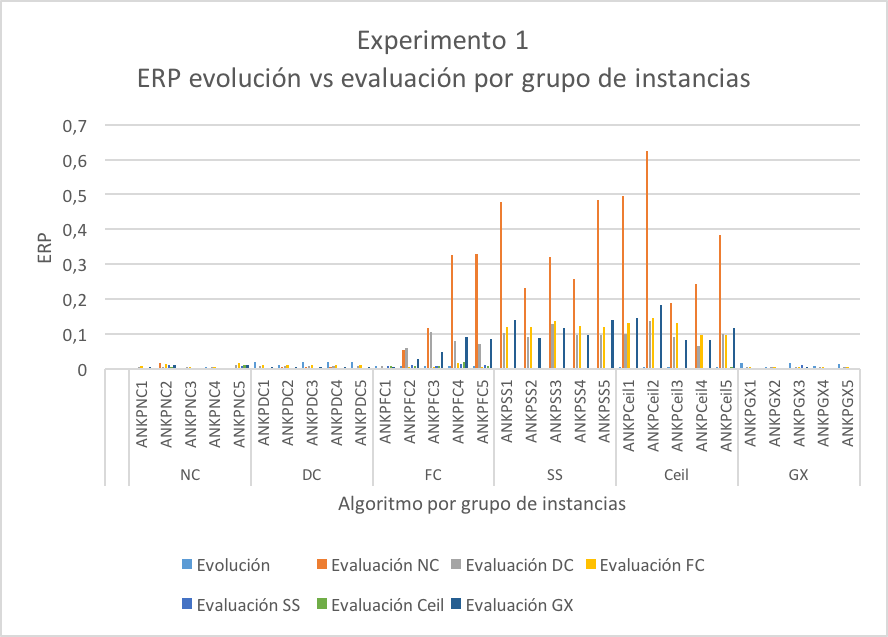
\includegraphics[width=13cm]{images/cap6/evol_vs_eval_exp1.png}
    \captionof{figure}{ERP de cada algoritmo por grupo sobre el conjunto de evaluación y evolución para el experimento 1 (Elaboración propia, 2015) }\label{fig:evol_vs_eval_exp1}
\endgroup

\begingroup
    \centering
    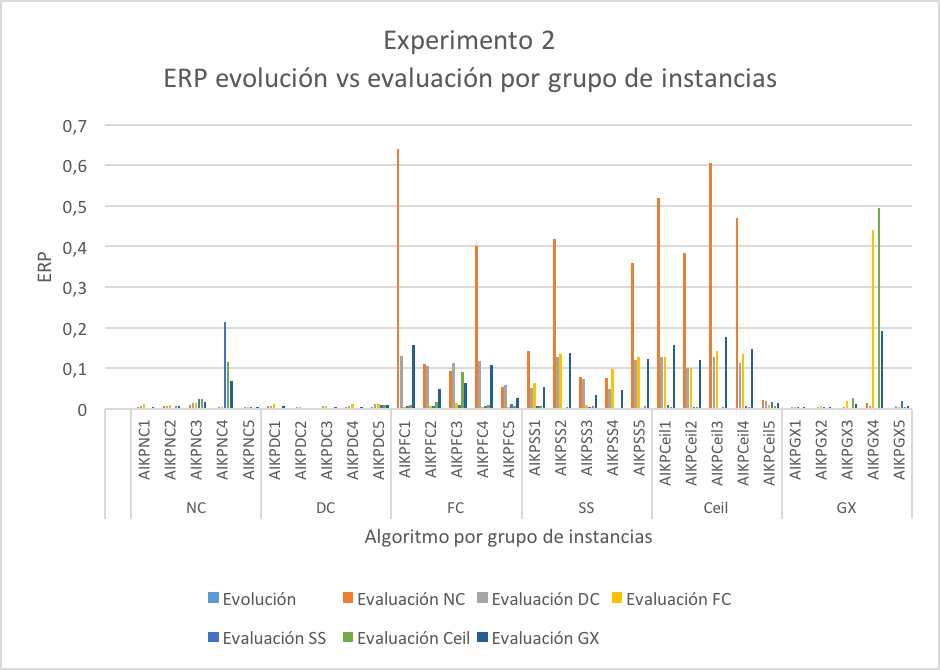
\includegraphics[width=13cm]{images/cap6/evol_vs_eval_exp2.png}
    \captionof{figure}{ERP de cada algoritmo por grupo sobre el conjunto de evaluación y evolución para el experimento 2 (Elaboración propia, 2015)}\label{fig:evol_vs_eval_exp2}
\endgroup

Los resultados obtenidos por los algoritmos producidos se sobre-especializan en el tipo de instancias de entrenamiento (evolución). Esta observación se desprende de la clasificación realizada para las instancias de acuerdo a su tipo. Como se muestra en la Tabla \ref{tab:evol_vs_eval_completa_exp1} para el experimento 1 y la Tabla \ref{tab:evol_vs_eval_completa_exp2} para el experimento 2, los resultados son similares para las instancias que tienen el mismo grupo de evolución y evaluación. Mientras que, para los otros casos, en su mayoría los resultados difieren.


\begin{table}[hbtp!]
\caption{Resultados del ERP para las instancias de evolución y evaluación para el mejor algoritmo de cada sub-experimento del experimento 1}\label{tab:evol_vs_eval_completa_exp1}
\small
\centering
\begin{center}
\rowcolors{2}{gray!25}{white}
\begin{tabular}{cc|cccccc}
\multicolumn{2}{c|}{{\textbf{}}} & \multicolumn{6}{c}{{\textbf{Grupos de instancias de evaluación}}} \\ \hline
{\textbf{Nombre}} & {\textbf{Evolución}} & {\textbf{NC}} & {\textbf{DC}} & {\textbf{FC}} & {\textbf{SS}} & {\textbf{Ceil}} & {\textbf{GX}} \\ \hline
ANKPNC1 & 0,004 & 0,005 & 0,007 & 0,009 & 0,004 & 0,002 & 0,005 \\
ANKPNC2 & 0,004 & 0,019 & 0,007 & 0,015 & 0,012 & 0,008 & 0,012 \\
ANKPNC3 & 0,004 & 0,004 & 0,007 & 0,008 & 0,003 & 0,002 & 0,005 \\
ANKPNC4 & 0,006 & 0,002 & 0,005 & 0,006 & 0,002 & 0,002 & 0,004 \\
ANKPNC5 & 0,005 & 0,005 & 0,012 & 0,017 & 0,010 & 0,011 & 0,011 \\ \hline
ANKPDC1 & 0,020 & 0,005 & 0,008 & 0,013 & 0,002 & 0,002 & 0,006 \\
ANKPDC2 & 0,012 & 0,007 & 0,010 & 0,013 & 0,003 & 0,003 & 0,007 \\
ANKPDC3 & 0,020 & 0,007 & 0,008 & 0,013 & 0,002 & 0,002 & 0,006 \\
ANKPDC4 & 0,020 & 0,006 & 0,008 & 0,013 & 0,002 & 0,002 & 0,006 \\
ANKPDC5 & 0,020 & 0,005 & 0,008 & 0,013 & 0,003 & 0,002 & 0,006 \\ \hline
ANKPFC1 & 0,010 & 0,003 & 0,008 & 0,005 & 0,008 & 0,008 & 0,006 \\
ANKPFC2 & 0,010 & 0,054 & 0,061 & 0,006 & 0,013 & 0,008 & 0,029 \\
ANKPFC3 & 0,009 & 0,118 & 0,106 & 0,007 & 0,009 & 0,010 & 0,050 \\
ANKPFC4 & 0,008 & 0,328 & 0,081 & 0,018 & 0,015 & 0,022 & 0,093 \\
ANKPFC5 & 0,010 & 0,330 & 0,073 & 0,006 & 0,013 & 0,008 & 0,086 \\ \hline
ANKPSS1 & 0,002 & 0,479 & 0,103 & 0,121 & 0,002 & 0,005 & 0,142 \\
ANKPSS2 & 0,002 & 0,233 & 0,092 & 0,121 & 0,002 & 0,005 & 0,091 \\
ANKPSS3 & 0,002 & 0,321 & 0,128 & 0,137 & 0,002 & 0,005 & 0,118 \\
ANKPSS4 & 0,002 & 0,257 & 0,097 & 0,125 & 0,002 & 0,005 & 0,097 \\
ANKPSS5 & 0,002 & 0,484 & 0,099 & 0,120 & 0,003 & 0,004 & 0,142 \\ \hline
ANKPCeil1 & 0,005 & 0,495 & 0,100 & 0,132 & 0,003 & 0,005 & 0,147 \\
ANKPCeil2 & 0,006 & 0,623 & 0,139 & 0,145 & 0,003 & 0,005 & 0,183 \\
ANKPCeil3 & 0,005 & 0,190 & 0,093 & 0,131 & 0,004 & 0,004 & 0,084 \\
ANKPCeil4 & 0,005 & 0,243 & 0,065 & 0,098 & 0,004 & 0,004 & 0,083 \\
ANKPCeil5 & 0,007 & 0,385 & 0,101 & 0,099 & 0,004 & 0,005 & 0,119 \\ \hline
ANKPGX1 & 0,018 & 0,002 & 0,006 & 0,006 & 0,004 & 0,002 & 0,004 \\
ANKPGX2 & 0,008 & 0,002 & 0,006 & 0,006 & 0,002 & 0,002 & 0,004 \\
ANKPGX3 & 0,017 & 0,002 & 0,006 & 0,006 & 0,011 & 0,003 & 0,006 \\
ANKPGX4 & 0,008 & 0,002 & 0,006 & 0,006 & 0,004 & 0,002 & 0,004 \\
ANKPGX5 & 0,015 & 0,002 & 0,006 & 0,006 & 0,002 & 0,003 & 0,004 \\
\hline
\end{tabular}
\end{center}
\caption*{(Elaboración propia, 2015)}
\end{table}

\begin{table}[hbtp!]
\caption{Resultados del ERP para las instancias de evolución y evaluación para el mejor algoritmo de cada sub-experimento del experimento 2}\label{tab:evol_vs_eval_completa_exp2}
\small
\centering
\begin{center}
\rowcolors{2}{gray!25}{white}
\begin{tabular}{cc|cccccc}
\multicolumn{2}{c|}{{\textbf{}}} & \multicolumn{6}{c}{{\textbf{Grupos de instancias de evaluación}}} \\ \hline
{\textbf{Nombre}} & {\textbf{Evolución}} & {\textbf{NC}} & {\textbf{DC}} & {\textbf{FC}} & {\textbf{SS}} & {\textbf{Ceil}} & {\textbf{GX}} \\ \hline
AIKPNC1 & 0,0050 & 0,0048 & 0,0083 & 0,0131 & 0,0030 & 0,0021 & 0,0063 \\
AIKPNC2 & 0,0050 & 0,0067 & 0,0087 & 0,0102 & 0,0024 & 0,0070 & 0,0070 \\
AIKPNC3 & 0,0059 & 0,0112 & 0,0161 & 0,0154 & 0,0237 & 0,0242 & 0,0181 \\
AIKPNC4 & 0,0060 & 0,0035 & 0,0057 & 0,0060 & 0,2135 & 0,1156 & 0,0689 \\
AIKPNC5 & 0,0060 & 0,0022 & 0,0058 & 0,0061 & 0,0042 & 0,0024 & 0,0041 \\ \hline
AIKPDC1 & 0,0197 & 0,0068 & 0,0082 & 0,0131 & 0,0024 & 0,0020 & 0,0065 \\
AIKPDC2 & 0,0182 & 0,0023 & 0,0056 & 0,0060 & 0,0024 & 0,0025 & 0,0038 \\
AIKPDC3 & 0,0172 & 0,0029 & 0,0065 & 0,0070 & 0,0025 & 0,0027 & 0,0043 \\
AIKPDC4 & 0,0197 & 0,0048 & 0,0083 & 0,0131 & 0,0030 & 0,0021 & 0,0063 \\
AIKPDC5 & 0,0285 & 0,0063 & 0,0117 & 0,0133 & 0,0105 & 0,0088 & 0,0101 \\ \hline
AIKPFC1 & 0,0101 & 0,6398 & 0,1303 & 0,0060 & 0,0087 & 0,0090 & 0,1588 \\
AIKPFC2 & 0,0101 & 0,1113 & 0,1070 & 0,0081 & 0,0087 & 0,0165 & 0,0503 \\
AIKPFC3 & 0,0089 & 0,0938 & 0,1123 & 0,0146 & 0,0110 & 0,0911 & 0,0646 \\
AIKPFC4 & 0,0101 & 0,4012 & 0,1178 & 0,0060 & 0,0087 & 0,0090 & 0,1085 \\
AIKPFC5 & 0,0101 & 0,0541 & 0,0604 & 0,0061 & 0,0132 & 0,0084 & 0,0285 \\ \hline
AIKPSS1 & 0,0023 & 0,1429 & 0,0527 & 0,0633 & 0,0080 & 0,0081 & 0,0550 \\
AIKPSS2 & 0,0101 & 0,4184 & 0,1287 & 0,1363 & 0,0012 & 0,0046 & 0,1378 \\
AIKPSS3 & 0,0089 & 0,0795 & 0,0741 & 0,0108 & 0,0044 & 0,0064 & 0,0350 \\
AIKPSS4 & 0,0101 & 0,0773 & 0,0503 & 0,0990 & 0,0013 & 0,0036 & 0,0463 \\
AIKPSS5 & 0,0101 & 0,3598 & 0,1196 & 0,1281 & 0,0034 & 0,0063 & 0,1235 \\ \hline
AIKPCeil1 & 0,0060 & 0,5195 & 0,1284 & 0,1270 & 0,0106 & 0,0058 & 0,1583 \\
AIKPCeil2 & 0,0071 & 0,3848 & 0,1022 & 0,1014 & 0,0041 & 0,0054 & 0,1196 \\
AIKPCeil3 & 0,0061 & 0,6045 & 0,1273 & 0,1434 & 0,0033 & 0,0041 & 0,1765 \\
AIKPCeil4 & 0,0060 & 0,4693 & 0,1144 & 0,1363 & 0,0086 & 0,0048 & 0,1467 \\
AIKPCeil5 & 0,0079 & 0,0221 & 0,0209 & 0,0107 & 0,0175 & 0,0074 & 0,0157 \\ \hline
AIKPGX1 & 0,0165 & 0,0023 & 0,0058 & 0,0060 & 0,0041 & 0,0024 & 0,0041 \\
AIKPGX2 & 0,0066 & 0,0035 & 0,0059 & 0,0079 & 0,0040 & 0,0023 & 0,0047 \\
AIKPGX3 & 0,0158 & 0,0022 & 0,0059 & 0,0188 & 0,0024 & 0,0281 & 0,0115 \\
AIKPGX4 & 0,0081 & 0,0157 & 0,0078 & 0,4410 & 0,0024 & 0,4945 & 0,1923 \\
AIKPGX5 & 0,0155 & 0,0027 & 0,0063 & 0,0061 & 0,0188 & 0,0049 & 0,0078 \\
\hline
\end{tabular}
\end{center}
\caption*{(Elaboración propia, 2015)}
\end{table}

Los algoritmos obtenidos mediante la evolución utilizando el grupo de instancias de adaptación $SS$ y $Ceil$, muestran una clara sobre especialización en las instancias que corresponden al mismo grupo. Estos grupos, como se mencionó en el diseño del experimento, poseen características muy similares. Específicamente, cuando se utilizaron para evolucionar los algoritmos, las instancias del grupo $SS$, surgieron los algoritmos $ANKPSS1$ a $ANKPSS5$ para el experimento 1 y los algoritmos $AIKPSS1$ a $AIKPSS5$ para el experimento 2. En la Tabla \ref{tab:evol_vs_eval_ss} se observan los resultados obtenidos para los cinco algoritmos de cada experimento con las instancias de evolución, solo para los algoritmos del grupo $SS$. Al observar los cinco algoritmos se detectan diferencias estructurales y también diferencias en el desempeño computacional. El mejor algoritmo obtenido es $ANKPSS4$ que presenta un error relativo promedio de $0,22\%$ en las 12 instancias de evolución. La estructura sintáctica del algoritmo se presenta en la Figura \ref{fig:ANKPSS4}. En esta figura se ve que el algoritmo utiliza como elementos la incorporación de nuevos ítems a la mochila por el menor beneficio, mayor peso, mayor ganancia ($beneficio / peso$), los que solo se preocupan de llenar la mochila. Entonces, el algoritmo opera estos terminales alternadamente hasta completar la mochila. Además, los terminales que agregan ítems de acuerdo al peso parecen ser los responsables finales de la especialización para este tipo de instancias. Es decir, el algoritmo $ANKPSS4$ se ha sobre especializado para las instancias de entrenamiento. Esta sobre especialización afecta en mayor medida a este grupo y al grupo $Ceil$, ya que, al tener una relación de igualdad (para el caso $SS$) y casi de igualdad (caso $Ceil$) entre el peso y el beneficio de los ítems a ingresar a la mochila, los algoritmos solo intentan llenar la mochila hasta alcanzar su capacidad. Como resultado, estos algoritmos en particular, obtienen los peores resultados al ser evaluados con los grupos de instancias distintas al de evolución.

\begin{table}[hbtp!]
\caption{Resultados del ERP de los algoritmos obtenidos por el grupo de instancias $SS$ para cada uno de los grupos de instancias de evaluación}\label{tab:evol_vs_eval_ss}
\small
\centering
\begin{center}
\begin{tabular}{ccc|cccccc}
\multicolumn{3}{c|}{{\textbf{}}} & \multicolumn{6}{c}{{\textbf{Grupos de instancias de evaluación}}} \\ \hline
{\textbf{Experimento}} & {\textbf{Nombre}} & {\textbf{Evolución}} & {\textbf{NC}} & {\textbf{DC}} & {\textbf{FC}} & {\textbf{SS}} & {\textbf{Ceil}} & {\textbf{GX}} \\ \hline
\begin{tabular}[c]{@{}c@{}} 
	Experimento 1 \\ SS 
\end{tabular} 		& 	\begin{tabular}[c]{@{}c@{}} ANKPSS1 \\ ANKPSS2 \\ ANKPSS3 \\ ANKPSS4 \\ ANKPSS5 \end{tabular} &
                        \begin{tabular}[c]{@{}c@{}} 0,002 \\ 0,002 \\ 0,002 \\ 0,002 \\ 0,002 \end{tabular} &
                        \begin{tabular}[c]{@{}c@{}} 0,479 \\ 0,233 \\ 0,321 \\ 0,257 \\ 0,484  \end{tabular} &
                        \begin{tabular}[c]{@{}c@{}} 0,103 \\ 0,092 \\ 0,128 \\ 0,097 \\ 0,099  \end{tabular} &
                        \begin{tabular}[c]{@{}c@{}} 0,121 \\ 0,121 \\ 0,137 \\ 0,125 \\ 0,120  \end{tabular} &
                        \begin{tabular}[c]{@{}c@{}} 0,002 \\ 0,002 \\ 0,002 \\ 0,002 \\ 0,003  \end{tabular} &
                        \begin{tabular}[c]{@{}c@{}} 0,005 \\ 0,005 \\ 0,005 \\ 0,005 \\ 0,004  \end{tabular} &
                        \begin{tabular}[c]{@{}c@{}} 0,142 \\ 0,091 \\ 0,118 \\ 0,097 \\ 0,142  \end{tabular} \\ \hline

\begin{tabular}[c]{@{}c@{}} 
	Experimento 2 \\ SS 
\end{tabular} 		& 	\begin{tabular}[c]{@{}c@{}} AIKPSS1 \\ AIKPSS2 \\ AIKPSS3 \\ AIKPSS4 \\ AIKPSS5 \end{tabular} &
                        \begin{tabular}[c]{@{}c@{}} 0,0023 \\ 0,0101 \\ 0,0089 \\ 0,0101 \\ 0,0101 \end{tabular} &
                        \begin{tabular}[c]{@{}c@{}} 0,1429 \\ 0,4184 \\ 0,0795 \\ 0,0773 \\ 0,3598 \end{tabular} &
                        \begin{tabular}[c]{@{}c@{}} 0,0527 \\ 0,1287 \\ 0,0741 \\ 0,0503 \\ 0,1196 \end{tabular} &
                        \begin{tabular}[c]{@{}c@{}} 0,0633 \\ 0,1363 \\ 0,0108 \\ 0,0990 \\ 0,1281 \end{tabular} &
                        \begin{tabular}[c]{@{}c@{}} 0,0080 \\ 0,0012 \\ 0,0044 \\ 0,0013 \\ 0,0034 \end{tabular} &
                        \begin{tabular}[c]{@{}c@{}} 0,0081 \\ 0,0046 \\ 0,0064 \\ 0,0036 \\ 0,0063 \end{tabular} &
                        \begin{tabular}[c]{@{}c@{}} 0,0550 \\ 0,1378 \\ 0,0350 \\ 0,0463 \\ 0,1235 \end{tabular} \\
\hline
\end{tabular}
\end{center}
\caption*{(Elaboración propia, 2015)}
\end{table}

\begingroup
    \centering
    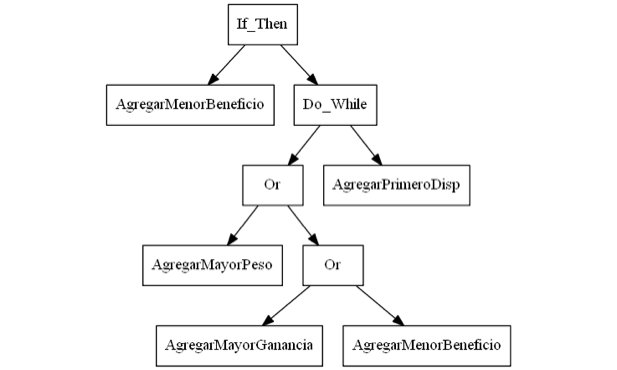
\includegraphics[width=13cm]{images/cap6/ANKPSS4.png}
    \captionof{figure}{Mejor algoritmo del experimento 1 para el grupo de instancias $SS$ (Elaboración propia, 2015)}\label{fig:ANKPSS4}
\endgroup

La sobre-especialización de los algoritmos se puede constatar simplemente revisando los resultados de su evaluación con instancias distintas del mismo grupo. Como se mencionó anteriormente, las tablas \ref{tab:evol_vs_eval_completa_exp1} y \ref{tab:evol_vs_eval_completa_exp2} presentan los resultados del ERP de los cinco algoritmos de cada sub-experimento para distintos grupos de instancias de cada experimento. Se observa que, en general, los algoritmos tienen un mejor rendimiento con las instancias del mismo grupo con el que se utilizaron las instancias para los casos de adaptación (evolución) en comparación a su rendimiento con las instancias de otros grupos. Las instancias del grupo $NC$, $DC$, $FC$, $Ceil$ y $GX$ siguen la misma lógica. Los resultados de la sobre especialización también son constatados para los otros grupos. Una clara excepción a esta sobre-especialización, es lo que ocurre en los grupos $NC$, $DC$, $FC$ y $GX$ al ser evaluados sobre los grupos $SS$ y $Ceil$. Esto se debe a que estas instancias “simplifican” el problema de estudio. Esta simplificación puede ser interpretada como “solo se debe llenar la mochila” y no a “llenar la mochila maximizando la ganancia” y se debe a que estas instancias poseen igualdad o una similitud entre el peso y beneficio que provee cada ítem al ser agregado a la mochila. La particularidad de estos grupos presenta menor dificultad para las funciones y terminales propuestos, generando que los algoritmos que han sido entrenados con otros grupos de instancias con características distintas, posean una mayor facilidad al momento de resolver las instancias de los grupos $SS$ y $Ceil$.

Los algoritmos obtenidos mediante la evolución utilizando el grupo de instancias combinadas $GX$, obtiene resultados similares a los obtenidos por otros algoritmos que evolucionaron con un solo grupo de adaptación. En la Tabla \ref{tab:evol_vs_eval_gx} se muestran los resultados que obtienen los algoritmos $ANKPGX1$ a $ANKPGX5$ para el proceso de evaluación con los distintos grupos del experimento 1. Es posible apreciar que los resultados obtenidos mediante la evolución utilizando instancias de diversos grupos, no posee una sobre especialización como ocurre con los otros algoritmos. Esto es debido a que los algoritmos se adaptan a una mayor cantidad de instancias, las que presentan una variación en la dificultad y características específicas que posee cada una para ser resuelta. En la Tabla \ref{tab:evol_vs_eval_gx} también se muestran los resultados que obtienen los algoritmos $AIKPGX1$ a $AIKPGX5$ para el proceso de evaluación con los distintos grupos del experimento 2, donde se puede constatar que ocurre un efecto similar al producido en el experimento 1.

\begin{table}[hbtp!]
\caption{Resultados del ERP de los algoritmos obtenidos por el grupo de instancias $GX$ para cada uno de los grupos de instancias de evaluación}\label{tab:evol_vs_eval_gx}
\small
\centering
\begin{center}
\begin{tabular}{ccc|cccccc}
\multicolumn{3}{c|}{{\textbf{}}} & \multicolumn{6}{c}{{\textbf{Grupos de instancias de evaluación}}} \\ \hline
{\textbf{Experimento}} & {\textbf{Nombre}} & {\textbf{Evolución}} & {\textbf{NC}} & {\textbf{DC}} & {\textbf{FC}} & {\textbf{SS}} & {\textbf{Ceil}} & {\textbf{GX}} \\ \hline
\begin{tabular}[c]{@{}c@{}} 
	Exp. 1 \\ GX 
\end{tabular} 		& 	\begin{tabular}[c]{@{}c@{}} ANKPGX1 \\ ANKPGX2 \\ ANKPGX3 \\ ANKPGX4 \\ ANKPGX5 \end{tabular} &
                        \begin{tabular}[c]{@{}c@{}} 0,0176 \\ 0,0077 \\ 0,0172 \\ 0,0081 \\ 0,0149 \end{tabular} &
                        \begin{tabular}[c]{@{}c@{}} 0,0022 \\ 0,0022 \\ 0,0022 \\ 0,0022 \\ 0,0022 \end{tabular} &
                        \begin{tabular}[c]{@{}c@{}} 0,0057 \\ 0,0059 \\ 0,0057 \\ 0,0057 \\ 0,0059 \end{tabular} &
                        \begin{tabular}[c]{@{}c@{}} 0,0060 \\ 0,0060 \\ 0,0060 \\ 0,0060 \\ 0,0061 \end{tabular} &
                        \begin{tabular}[c]{@{}c@{}} 0,0041 \\ 0,0024 \\ 0,0111 \\ 0,0041 \\ 0,0024 \end{tabular} &
                        \begin{tabular}[c]{@{}c@{}} 0,0024 \\ 0,0025 \\ 0,0029 \\ 0,0024 \\ 0,0026 \end{tabular} &
                        \begin{tabular}[c]{@{}c@{}} 0,0041 \\ 0,0038 \\ 0,0056 \\ 0,0041 \\ 0,0038 \end{tabular} \\ \hline

\begin{tabular}[c]{@{}c@{}} 
    Exp. 2 \\ GX 
\end{tabular}       &   \begin{tabular}[c]{@{}c@{}} AIKPGX1 \\ AIKPGX2 \\ AIKPGX3 \\ AIKPGX4 \\ AIKPGX5 \end{tabular} &
                        \begin{tabular}[c]{@{}c@{}} 0,0165 \\ 0,0066 \\ 0,0158 \\ 0,0081 \\ 0,0155 \end{tabular} &
                        \begin{tabular}[c]{@{}c@{}} 0,0023 \\ 0,0035 \\ 0,0022 \\ 0,0157 \\ 0,0027 \end{tabular} &
                        \begin{tabular}[c]{@{}c@{}} 0,0058 \\ 0,0059 \\ 0,0059 \\ 0,0078 \\ 0,0063 \end{tabular} &
                        \begin{tabular}[c]{@{}c@{}} 0,0060 \\ 0,0079 \\ 0,0188 \\ 0,4410 \\ 0,0061 \end{tabular} &
                        \begin{tabular}[c]{@{}c@{}} 0,0041 \\ 0,0040 \\ 0,0024 \\ 0,0024 \\ 0,0188 \end{tabular} &
                        \begin{tabular}[c]{@{}c@{}} 0,0024 \\ 0,0023 \\ 0,0281 \\ 0,4945 \\ 0,0049 \end{tabular} &
                        \begin{tabular}[c]{@{}c@{}} 0,0041 \\ 0,0047 \\ 0,0115 \\ 0,1923 \\ 0,0078 \end{tabular} \\
\hline
\end{tabular}
\end{center}
\caption*{(Elaboración propia, 2015)}
\end{table}

Los algoritmos producidos son muy rápidos para resolver los problemas de la mochila. En la Tabla \ref{tab:evol_vs_eval_tiempos_exp1} se muestra el tiempo que le toma al mejor algoritmo de cada ejecución resolver las instancias de cada uno de los grupos ($NC$, $DC$, $FC$, $SS$ y $Ceil$) para el experimento 1. Es importante destacar que cada uno de los grupos contiene 780 instancias que varían en tamaño de $100$ a $10.000$ ítems y el grupo GX contiene las $3.900$ instancias de los otros grupos (véase \ref{cap:sel_casos_adapt_pm01}). El tiempo empleado es en promedio cinco minutos, alcanzando menos de dos minutos el más rápido y casi 12 minutos el más lento de ellos. Adicionalmente, se puede ver que el grupo GX de evaluación (compuesto por todas las instancias de evaluación de los otros grupos) obtiene tiempos promedios de 22 minutos, obteniendo menos de 10 minutos el más rápido y casi una hora el más lento. Los algoritmos más rápidos resuelven en una milésima de segundo cada instancia, mientras que los más lentos las resuelven en aproximadamente un segundo. En la Tabla \ref{tab:evol_vs_eval_tiempos_exp2} se puede observar los tiempos en que los mejores algoritmos del experimento 2 resuelven las instancias para cada uno de los grupos, aunque, si bien los tiempos empleados en la evaluación no son iguales, son similares. Esto se debe a que todos los algoritmos producidos tienen una complejidad polinomial. %Agregar que grupo es más rápido de resolver o cosas así

\begin{table}[hbtp!]
\caption{Tiempo que demora en resolver el mejor algoritmo de cada sub-experimento del experimento 1, los grupos de evaluación}\label{tab:evol_vs_eval_tiempos_exp1}
\small
\centering
\begin{center}
\rowcolors{2}{gray!25}{white}
\begin{tabular}{c|cccccc}
{\textbf{}} & \multicolumn{6}{c}{{\textbf{Tiempo en minutos}}} \\ \hline
{\textbf{Nombre}} & {\textbf{NC}} & {\textbf{DC}} & {\textbf{FC}} & {\textbf{SS}} & {\textbf{Ceil}} & {\textbf{GX}} \\ \hline
ANKPNC1 & 5,36 & 4,26 & 5,83 & 3,41 & 4,77 & 23,62 \\
ANKPNC2 & 7,39 & 5,34 & 7,55 & 3,75 & 5,93 & 29,97 \\
ANKPNC3 & 5,32 & 4,12 & 5,73 & 3,33 & 4,58 & 23,08 \\
ANKPNC4 & 4,35 & 3,47 & 4,68 & 2,81 & 3,95 & 19,26 \\
ANKPNC5 & 4,72 & 3,59 & 4,92 & 2,82 & 3,86 & 19,91 \\
ANKPDC1 & 5,80 & 4,40 & 6,49 & 3,36 & 5,09 & 25,14 \\
ANKPDC2 & 6,67 & 5,33 & 6,56 & 3,44 & 5,73 & 27,72 \\
ANKPDC3 & 6,89 & 5,36 & 7,81 & 4,17 & 6,01 & 30,24 \\
ANKPDC4 & 4,67 & 3,65 & 5,26 & 2,89 & 4,18 & 20,65 \\
ANKPDC5 & 4,66 & 3,61 & 5,07 & 2,80 & 3,87 & 20,02 \\
ANKPFC1 & 5,78 & 4,44 & 6,36 & 3,39 & 5,20 & 25,17 \\
ANKPFC2 & 5,13 & 5,05 & 5,33 & 4,56 & 5,54 & 25,61 \\
ANKPFC3 & 11,82 & 11,68 & 11,46 & 11,37 & 11,25 & 57,58 \\
ANKPFC4 & 4,09 & 4,43 & 4,59 & 3,79 & 4,23 & 21,13 \\
ANKPFC5 & 4,54 & 4,72 & 4,84 & 3,80 & 4,50 & 22,39 \\
ANKPSS1 & 1,93 & 1,87 & 1,89 & 1,90 & 1,88 & 9,49 \\
ANKPSS2 & 2,49 & 1,78 & 1,80 & 1,86 & 1,91 & 9,83 \\
ANKPSS3 & 6,60 & 5,86 & 4,34 & 4,91 & 4,99 & 26,71 \\
ANKPSS4 & 2,32 & 1,72 & 1,80 & 1,81 & 1,80 & 9,44 \\
ANKPSS5 & 1,82 & 1,82 & 1,87 & 1,87 & 1,81 & 9,19 \\
ANKPCeil1 & 2,94 & 3,22 & 2,64 & 2,32 & 2,83 & 13,96 \\
ANKPCeil2 & 2,63 & 3,16 & 2,33 & 2,55 & 2,64 & 13,31 \\
ANKPCeil3 & 7,91 & 4,97 & 5,04 & 4,08 & 4,96 & 26,97 \\
ANKPCeil4 & 3,80 & 3,61 & 3,22 & 2,46 & 3,36 & 16,44 \\
ANKPCeil5 & 4,31 & 4,59 & 3,56 & 2,82 & 3,95 & 19,24 \\
ANKPGX1 & 4,59 & 3,70 & 5,14 & 2,92 & 4,20 & 20,55 \\
ANKPGX2 & 4,55 & 3,64 & 5,29 & 2,88 & 4,44 & 20,80 \\
ANKPGX3 & 9,02 & 7,04 & 10,03 & 4,84 & 7,72 & 38,64 \\
ANKPGX4 & 4,55 & 3,62 & 5,14 & 2,91 & 4,20 & 20,41 \\
ANKPGX5 & 5,58 & 4,35 & 6,14 & 3,33 & 4,68 & 24,09 \\
\hline
\end{tabular}
\end{center}
\caption*{(Elaboración propia, 2015)}
\end{table}

\begin{table}[hbtp!]
\caption{Tiempo que demora en resolver el mejor algoritmo de cada sub-experimento del experimento 2, los grupos de evaluación}\label{tab:evol_vs_eval_tiempos_exp2}
\small
\centering
\begin{center}
\rowcolors{2}{gray!25}{white}
\begin{tabular}{c|cccccc}
{\textbf{}} & \multicolumn{6}{c}{{\textbf{Tiempo en minutos}}} \\ \hline
{\textbf{Nombre}} & {\textbf{NC}} & {\textbf{DC}} & {\textbf{FC}} & {\textbf{SS}} & {\textbf{Ceil}} & {\textbf{GX}} \\ \hline
AIKPNC1 & 4,68 & 3,67 & 5,34 & 3,00 & 4,84 & 21,53 \\
AIKPNC2 & 10,31 & 8,04 & 11,18 & 6,16 & 10,97 & 46,66 \\
AIKPNC3 & 6,87 & 5,30 & 7,73 & 4,15 & 5,90 & 29,95 \\
AIKPNC4 & 10,20 & 7,95 & 11,22 & 2,10 & 4,82 & 36,28 \\
AIKPNC5 & 4,58 & 3,59 & 4,90 & 2,81 & 3,92 & 19,80 \\
AIKPDC1 & 6,87 & 5,43 & 7,72 & 4,35 & 6,22 & 30,60 \\
AIKPDC2 & 5,83 & 4,39 & 6,33 & 3,51 & 5,17 & 25,23 \\
AIKPDC3 & 5,68 & 4,41 & 6,38 & 3,55 & 5,16 & 25,17 \\
AIKPDC4 & 4,62 & 3,66 & 5,17 & 2,99 & 4,24 & 20,68 \\
AIKPDC5 & 4,60 & 3,51 & 4,99 & 2,82 & 3,84 & 19,77 \\
AIKPFC1 & 4,29 & 6,10 & 6,14 & 6,16 & 6,13 & 28,82 \\
AIKPFC2 & 6,42 & 7,00 & 6,38 & 6,40 & 6,20 & 32,41 \\
AIKPFC3 & 17,12 & 9,37 & 5,32 & 5,20 & 3,85 & 40,87 \\
AIKPFC4 & 4,52 & 5,07 & 5,10 & 5,06 & 4,97 & 24,71 \\
AIKPFC5 & 5,12 & 4,88 & 5,04 & 4,05 & 4,53 & 23,61 \\
AIKPSS1 & 9,61 & 32,65 & 2,95 & 2,95 & 4,09 & 52,24 \\
AIKPSS2 & 3,02 & 3,00 & 2,46 & 2,56 & 2,80 & 13,84 \\
AIKPSS3 & 5,65 & 4,89 & 6,12 & 4,66 & 5,15 & 26,47 \\
AIKPSS4 & 4,05 & 2,93 & 3,51 & 2,49 & 3,20 & 16,18 \\
AIKPSS5 & 3,05 & 3,02 & 2,40 & 2,58 & 2,60 & 13,65 \\
AIKPCeil1 & 2,93 & 3,64 & 2,71 & 2,56 & 3,29 & 15,12 \\
AIKPCeil2 & 4,08 & 4,61 & 3,68 & 3,01 & 4,19 & 19,57 \\
AIKPCeil3 & 2,30 & 2,75 & 2,24 & 2,40 & 2,45 & 12,13 \\
AIKPCeil4 & 2,86 & 3,05 & 2,54 & 2,54 & 2,87 & 13,86 \\
AIKPCeil5 & 4,68 & 3,65 & 5,25 & 3,39 & 4,19 & 21,16 \\
AIKPGX1 & 4,73 & 3,72 & 5,25 & 2,87 & 4,31 & 20,88 \\
AIKPGX2 & 5,26 & 4,19 & 5,73 & 3,13 & 4,66 & 22,97 \\
AIKPGX3 & 4,64 & 3,71 & 4,92 & 2,91 & 3,90 & 20,08 \\
AIKPGX4 & 10,03 & 7,79 & 0,34 & 6,05 & 0,44 & 24,64 \\
AIKPGX5 & 5,90 & 4,58 & 6,38 & 3,79 & 4,87 & 25,52 \\
\hline
\end{tabular}
\end{center}
\caption*{(Elaboración propia, 2015)}
\end{table}

Los algoritmos obtenidos mediante el proceso co-evolutivo utilizando el método de islas tienen un desempeño computacional similar a los algoritmos obtenidos mediante el proceso tradicional. En las tablas \ref{tab:mejores_exp_hits_pm01} y \ref{tab:mejores_exp_erp_pm01} se muestran los resultados de cinco mejores algoritmos obtenidos para cada experimento. Estos algoritmos fueron los mejores de cada uno de los sub-experimentos de acuerdo a los resultados obtenidos al ser evaluados con los grupos de evaluación. Específicamente, en la Tabla \ref{tab:mejores_exp_hits_pm01} se presentan los mejores individuos de acuerdo a la cantidad de instancias que logran resolver de forma óptima. Mientras que en la Tabla \ref{tab:mejores_exp_erp_pm01} se presentan los mejores individuos que obtuvieron el menor ERP en el grupo de evaluación. En estas tablas se presentan los indicadores de cada algoritmo y el error relativo que se obtuvo al evaluar los algoritmos con el mismo conjunto de instancias de evaluación y la cantidad de soluciones óptimas que encuentra. Tal como se observa, el error relativo promedio de los algoritmos del primer experimento es similar al del segundo experimento. Los resultados obtenidos por ambos experimentos siguen una distribución normal, así lo muestra el \textit{test de Shapiro-Wilk}. En consecuencia,  el \textit{test} de ANOVA que proporciona bajo un 95\% de confiabilidad que no existe diferencia significativa en los datos obtenidos, por lo que no es posible rechazar la hipótesis nula. El resultado contrasta descubrimientos realizados por otros autores para algoritmos genéticos, lo que puede ser inferido puesto que algunos de los resultados obtenidos utilizando el método de la PG con co-evolución muestran una mejora en la calidad de los algoritmos, la que es estadísticamente despreciable.

\begin{table}[hbtp!]
\caption{Mejores individuos por cantidad de soluciones encontradas en grupo de evaluación}\label{tab:mejores_exp_hits_pm01}
\small
\centering
\begin{center}
\begin{tabular}{ccc|ccc|ccc}
\multicolumn{3}{c}{{\textbf{ }}} & \multicolumn{3}{|c|}{{\textbf{Error Relativo}}} & \multicolumn{3}{c}{{\textbf{ }}} \\
{\textbf{Grupo}} & {\textbf{Exp.}} & {\textbf{Nombre}} & {\textbf{Peor}} & {\textbf{Prom.}} & {\textbf{Mejor}} & {\textbf{Soluciones}} & {\textbf{Nodos}} & {\textbf{Altura}}\\ \hline
NC & 	\begin{tabular}[c]{@{}c@{}} 1 \\ 2 \end{tabular} &
		\begin{tabular}[c]{@{}c@{}} ANKPNC4 \\ AIKPNC5 \end{tabular} &
		\begin{tabular}[c]{@{}c@{}} 0,2114 \\ 0,8044   \end{tabular} &
		\begin{tabular}[c]{@{}c@{}} 0,0036 \\ 0,0041   \end{tabular} &
		\begin{tabular}[c]{@{}c@{}} 0 \\ 0 			   \end{tabular} &
		\begin{tabular}[c]{@{}c@{}} 205 \\ 189         \end{tabular} &
		\begin{tabular}[c]{@{}c@{}} 5 \\ 3 			   \end{tabular} &
		\begin{tabular}[c]{@{}c@{}} 15 \\ 5 		   \end{tabular} \\ \hline

DC & 	\begin{tabular}[c]{@{}c@{}} 1 \\ 2 \end{tabular} &
		\begin{tabular}[c]{@{}c@{}} ANKPDC2 \\ AIKPDC1 \end{tabular} &
		\begin{tabular}[c]{@{}c@{}} 1,0000 \\ 0,5933   \end{tabular} &
		\begin{tabular}[c]{@{}c@{}} 0,0073 \\ 0,0065   \end{tabular} &
		\begin{tabular}[c]{@{}c@{}} 0 \\ 0 			   \end{tabular} &
		\begin{tabular}[c]{@{}c@{}} 303 \\ 185         \end{tabular} &
		\begin{tabular}[c]{@{}c@{}} 6 \\ 5 			   \end{tabular} &
		\begin{tabular}[c]{@{}c@{}} 15 \\ 13 		   \end{tabular} \\ \hline

FC & 	\begin{tabular}[c]{@{}c@{}} 1 \\ 2 \end{tabular} &
		\begin{tabular}[c]{@{}c@{}} ANKPFC1 \\ AIKPFC5 \end{tabular} &
		\begin{tabular}[c]{@{}c@{}} 0,2805 \\ 0,8035   \end{tabular} &
		\begin{tabular}[c]{@{}c@{}} 0,0063 \\ 0,0285   \end{tabular} &
		\begin{tabular}[c]{@{}c@{}} 0 \\ 0 			   \end{tabular} &
		\begin{tabular}[c]{@{}c@{}} 96 \\ 12         \end{tabular} &
		\begin{tabular}[c]{@{}c@{}} 4 \\ 2 			   \end{tabular} &
		\begin{tabular}[c]{@{}c@{}} 14 \\ 3 		   \end{tabular} \\ \hline

SS & 	\begin{tabular}[c]{@{}c@{}} 1 \\ 2 \end{tabular} &
		\begin{tabular}[c]{@{}c@{}} ANKPSS4 \\ AIKPSS4 \end{tabular} &
		\begin{tabular}[c]{@{}c@{}} 0,9027 \\ 0,7692   \end{tabular} &
		\begin{tabular}[c]{@{}c@{}} 0,0972 \\ 0,0463   \end{tabular} &
		\begin{tabular}[c]{@{}c@{}} 0 \\ 0 			   \end{tabular} &
		\begin{tabular}[c]{@{}c@{}} 68 \\ 102          \end{tabular} &
		\begin{tabular}[c]{@{}c@{}} 3 \\ 5 			   \end{tabular} &
		\begin{tabular}[c]{@{}c@{}} 5 \\ 11 		   \end{tabular} \\ \hline

Ceil & 	\begin{tabular}[c]{@{}c@{}} 1 \\ 2 \end{tabular} &
		\begin{tabular}[c]{@{}c@{}} ANKPCeil2 \\ AIKPCeil3 \end{tabular} &
		\begin{tabular}[c]{@{}c@{}} 0,9790 \\ 0,9790   \end{tabular} &
		\begin{tabular}[c]{@{}c@{}} 0,1830 \\ 0,1765   \end{tabular} &
		\begin{tabular}[c]{@{}c@{}} 0 \\ 0 			   \end{tabular} &
		\begin{tabular}[c]{@{}c@{}} 67 \\ 65          \end{tabular} &
		\begin{tabular}[c]{@{}c@{}} 5 \\ 6 			   \end{tabular} &
		\begin{tabular}[c]{@{}c@{}} 13 \\ 15 		   \end{tabular} \\ \hline

GX & 	\begin{tabular}[c]{@{}c@{}} 1 \\ 2 \end{tabular} &
		\begin{tabular}[c]{@{}c@{}} ANKPGX3 \\ AIKPGX2 \end{tabular} &
		\begin{tabular}[c]{@{}c@{}} 0,8363 \\ 0,8044   \end{tabular} &
		\begin{tabular}[c]{@{}c@{}} 0,0056 \\ 0,0047   \end{tabular} &
		\begin{tabular}[c]{@{}c@{}} 0 \\ 0 			   \end{tabular} &
		\begin{tabular}[c]{@{}c@{}} 215 \\ 192          \end{tabular} &
		\begin{tabular}[c]{@{}c@{}} 4 \\ 5			   \end{tabular} &
		\begin{tabular}[c]{@{}c@{}} 9 \\ 15 		   \end{tabular} \\
\hline
\end{tabular}
\end{center}
\caption*{(Elaboración propia, 2015)}
\end{table}

\begin{table}[hbtp!]
\caption{Mejores individuos por menor ERP en grupo de evaluación}\label{tab:mejores_exp_erp_pm01}
\small
\centering
\begin{center}
\begin{tabular}{ccc|ccc|ccc}
\multicolumn{3}{c}{{\textbf{ }}} & \multicolumn{3}{|c|}{{\textbf{Error Relativo}}} & \multicolumn{3}{c}{{\textbf{ }}} \\
{\textbf{Grupo}} & {\textbf{Exp.}} & {\textbf{Nombre}} & {\textbf{Peor}} & {\textbf{Prom.}} & {\textbf{Mejor}} & {\textbf{Soluciones}} & {\textbf{Nodos}} & {\textbf{Altura}}\\ \hline
NC & 	\begin{tabular}[c]{@{}c@{}} 1 \\ 2 \end{tabular} &
		\begin{tabular}[c]{@{}c@{}} ANKPNC4 \\ AIKPNC5 \end{tabular} &
		\begin{tabular}[c]{@{}c@{}} 0,2114 \\ 0,8044   \end{tabular} &
		\begin{tabular}[c]{@{}c@{}} 0,0036 \\ 0,0041   \end{tabular} &
		\begin{tabular}[c]{@{}c@{}} 0 \\ 0 			   \end{tabular} &
		\begin{tabular}[c]{@{}c@{}} 205 \\ 189         \end{tabular} &
		\begin{tabular}[c]{@{}c@{}} 5 \\ 3 			   \end{tabular} &
		\begin{tabular}[c]{@{}c@{}} 15 \\ 5 		   \end{tabular} \\ \hline

DC & 	\begin{tabular}[c]{@{}c@{}} 1 \\ 2 \end{tabular} &
		\begin{tabular}[c]{@{}c@{}} ANKPDC1 \\ AIKPDC2 \end{tabular} &
		\begin{tabular}[c]{@{}c@{}} 0,5933 \\  0,2114  \end{tabular} &
		\begin{tabular}[c]{@{}c@{}} 0,0060 \\  0,0038  \end{tabular} &
		\begin{tabular}[c]{@{}c@{}} 0 \\ 0 			   \end{tabular} &
		\begin{tabular}[c]{@{}c@{}} 188 \\ 178         \end{tabular} &
		\begin{tabular}[c]{@{}c@{}} 6 \\ 6 			   \end{tabular} &
		\begin{tabular}[c]{@{}c@{}} 14 \\ 15 		   \end{tabular} \\ \hline

FC & 	\begin{tabular}[c]{@{}c@{}} 1 \\ 2 \end{tabular} &
		\begin{tabular}[c]{@{}c@{}} ANKPFC1 \\ AIKPFC5 \end{tabular} &
		\begin{tabular}[c]{@{}c@{}} 0,2805 \\ 0,8035   \end{tabular} &
		\begin{tabular}[c]{@{}c@{}} 0,0063 \\ 0,0285   \end{tabular} &
		\begin{tabular}[c]{@{}c@{}} 0 \\ 0 			   \end{tabular} &
		\begin{tabular}[c]{@{}c@{}} 96 \\ 12         \end{tabular} &
		\begin{tabular}[c]{@{}c@{}} 4 \\ 2 			   \end{tabular} &
		\begin{tabular}[c]{@{}c@{}} 14 \\ 3 		   \end{tabular} \\ \hline

SS & 	\begin{tabular}[c]{@{}c@{}} 1 \\ 2 \end{tabular} &
		\begin{tabular}[c]{@{}c@{}} ANKPSS2 \\ AIKPSS3 \end{tabular} &
		\begin{tabular}[c]{@{}c@{}} 0,8590 \\ 0,7056   \end{tabular} &
		\begin{tabular}[c]{@{}c@{}} 0,0905 \\ 0,0350   \end{tabular} &
		\begin{tabular}[c]{@{}c@{}} 0 \\ 0 			   \end{tabular} &
		\begin{tabular}[c]{@{}c@{}} 63 \\ 10           \end{tabular} &
		\begin{tabular}[c]{@{}c@{}} 4 \\ 4 			   \end{tabular} &
		\begin{tabular}[c]{@{}c@{}} 10 \\ 13		   \end{tabular} \\ \hline

Ceil & 	\begin{tabular}[c]{@{}c@{}} 1 \\ 2 \end{tabular} &
		\begin{tabular}[c]{@{}c@{}} ANKPCeil4 \\ AIKPCeil5 \end{tabular} &
		\begin{tabular}[c]{@{}c@{}} 0,9299 \\ 0,9391   \end{tabular} &
		\begin{tabular}[c]{@{}c@{}} 0,0830 \\ 0,0157   \end{tabular} &
		\begin{tabular}[c]{@{}c@{}} 0 \\ 0 			   \end{tabular} &
		\begin{tabular}[c]{@{}c@{}} 48 \\ 53           \end{tabular} &
		\begin{tabular}[c]{@{}c@{}} 4 \\ 6 			   \end{tabular} &
		\begin{tabular}[c]{@{}c@{}} 11 \\ 14 		   \end{tabular} \\ \hline

GX & 	\begin{tabular}[c]{@{}c@{}} 1 \\ 2 \end{tabular} &
		\begin{tabular}[c]{@{}c@{}} ANKPGX2 \\ AIKPGX1 \end{tabular} &
		\begin{tabular}[c]{@{}c@{}} 0,2114 \\ 0,8044   \end{tabular} &
		\begin{tabular}[c]{@{}c@{}} 0,0038 \\ 0,0041   \end{tabular} &
		\begin{tabular}[c]{@{}c@{}} 0 \\ 0 			   \end{tabular} &
		\begin{tabular}[c]{@{}c@{}} 200 \\ 184          \end{tabular} &
		\begin{tabular}[c]{@{}c@{}} 5 \\ 5			   \end{tabular} &
		\begin{tabular}[c]{@{}c@{}} 8 \\ 11 		   \end{tabular} \\
\hline
\end{tabular}
\end{center}
\caption*{(Elaboración propia, 2015)}
\end{table}

\subsection{Estructura de los algoritmos generados}

Para facilitar la comprensión de los algoritmos, en esta sección se presenta una figura que muestra el árbol sintáctico del algoritmo junto a una breve explicación de cómo funciona. Los algoritmos descritos en esta sección incluyen sólo al mejor algoritmo de los que fueron señalados en la Tabla \ref{tab:mejores_exp_hits_pm01} y \ref{tab:mejores_exp_erp_pm01} para cada experimento. Estos algoritmos son $ANKPDC2$ y $AIKPGX2$ para la Tabla \ref{tab:mejores_exp_erp_pm01}, que representan a los mejores algoritmos para el problema de la mochila utilizando como criterio encontrar la mayor cantidad de soluciones óptimas para las instancias de evaluación. Para la Tabla \ref{tab:mejores_exp_hits_pm01} son seleccionados los algoritmos $ANKPNC4$ y $AIKPDC2$ que representan a los mejores algoritmos para el problema de la mochila siguiendo el criterio de obtener el menor ERP para las instancias de evaluación.

\subsubsection{ANKPDC2}

El $ANKPDC2$ es el mejor algoritmo obtenido en el experimento 1, utilizando como criterio la cantidad de soluciones que encuentra en el grupo de evaluación. En la Figura \ref{fig:ANKPDC2} se puede ver el algoritmo por medio de su árbol sintáctico. Este algoritmo posee 15 nodos y una altura de 6, compuesto de 7 terminales y 8 funciones. Este algoritmo sigue una lógica puramente constructiva, utilizando distintos criterios tiene por objetivo el llenado de la mochila.
Los pasos a realizar por este algoritmo inician con el ingreso del elemento con el mayor beneficio. Si se realiza el ingreso, se procede a realizar un ciclo \textit{“while”} con la condición de \textit{“true”}, es decir, se ejecuta el árbol derecho hasta que no se produzcan más cambios. El árbol derecho consta de el ingreso de ítems a la mochila iniciando por el de mayor ganancia, posteriormente el primero de la lista de disponibles y posteriormente se ingresa a otro ciclo que llena todos los elementos restantes de acuerdo a su menor peso. Este proceso se realiza hasta alcanzar la capacidad máxima de la mochila. El terminal “AgregarMayorGanancia” ubicado en la rama derecha no es ejecutado. La lógica de este algoritmo es un goloso con el criterio principal de agregar los ítem que provean la mayor ganancia.

\begingroup
    \centering
    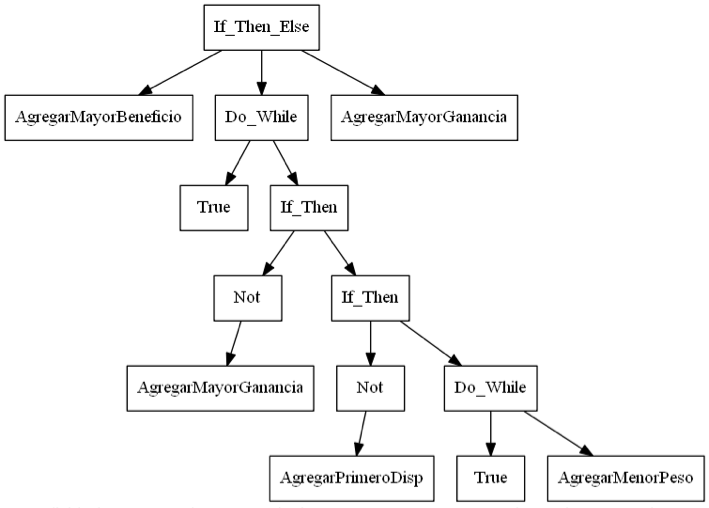
\includegraphics[width=13cm]{images/cap6/ANKPDC2.png}
    \captionof{figure}{Mejor algoritmo del experimento 1 por cantidad de soluciones óptimas obtenidas (Elaboración propia, 2015)}\label{fig:ANKPDC2}
\endgroup

\subsubsection{AIKPGX2}

El $AIKPGX2$ es el mejor algoritmo obtenido en el experimento 2, utilizando como criterio la cantidad de soluciones que encuentra en el grupo de evaluación. En la Figura \ref{fig:AIKPGX2} se puede ver el algoritmo por medio de su árbol sintáctico. Este algoritmo posee 15 nodos y una altura de 5, se encuentra compuesto de 8 terminales y 7 funciones. A diferencia del algoritmo anterior, este algoritmo utiliza un terminal que elimina siguiendo una lógica constructiva y de refinamiento.
Los pasos a realizar por este algoritmo inician con un ciclo \textit{“while”} donde se ingresan ítems de acuerdo a la mayor ganancia y menor peso. Posteriormente, se ejecuta el árbol derecho agregando ítems de acuerdo a su mayor ganancia y mayor beneficio. Si cinco ítems son agregados, se procede a eliminar el ítem con la peor ganancia y se ejecuta nuevamente el algoritmo. La lógica que sigue este algoritmo es de un goloso, que en un determinado momento realiza un refinamiento.

\begingroup
    \centering
    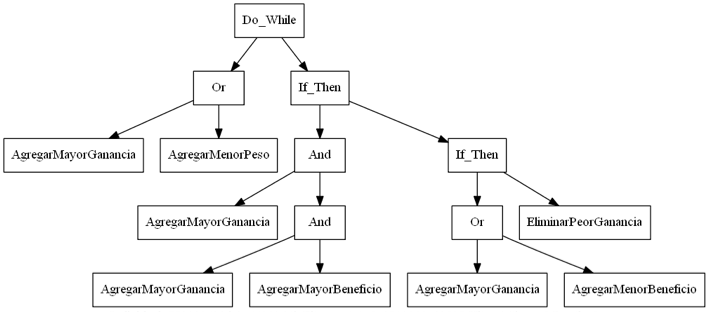
\includegraphics[width=13cm]{images/cap6/AIKPGX2.png}
    \captionof{figure}{Mejor algoritmo del experimento 2 por cantidad de soluciones óptimas obtenidas (Elaboración propia, 2015)}\label{fig:AIKPGX2}
\endgroup

\subsubsection{ANKPNC4}

El $ANKPNC4$ es el mejor algoritmo obtenido en el experimento 1, utilizando como criterio la obtención del menor ERP al ser evaluado en el grupo de evaluación. En la Figura \ref{fig:ANKPNC4} se puede ver el árbol sintáctico del algoritmo. Este algoritmo posee 15 nodos y una altura de 5, está compuesto de 9 terminales y 6 funciones. Este algoritmo sigue una lógica constructiva y de refinamiento.
El algoritmo inicia su procedimiento mediante un ciclo \textit{“while”}. Comienza insertando 3 ítems a la mochila con los criterios de mayor ganancia, primero disponible y menor peso para posteriormente eliminar el con peor beneficio de éstos. A continuación, agrega ítems a la mochila de acuerdo a su mayor ganancia, si no es posible agregar al de mayor ganancia, se procede a agregar el de menor peso. Finalmente, vuelve a comenzar el algoritmo. La lógica de este algoritmo es un goloso con el criterio principal de agregar los ítem que provean la mayor ganancia y en un determinado momento intenta realizar un refinamiento.

\begingroup
    \centering
    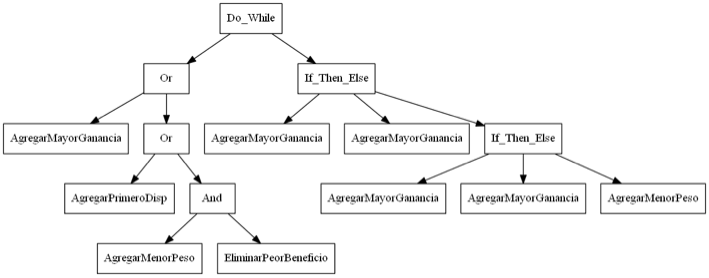
\includegraphics[width=13cm]{images/cap6/ANKPNC4.png}
    \captionof{figure}{Mejor algoritmo del experimento 1 por menor ERP (Elaboración propia, 2015)}\label{fig:ANKPNC4}
\endgroup

\subsubsection{AIKPDC2}

El $AIKPDC2$ es el mejor algoritmo obtenido en el experimento 2, utilizando como criterio la obtención del menor ERP al ser evaluado en el grupo de evaluación. En la Figura \ref{fig:AIKPDC2} se puede ver el árbol sintáctico del algoritmo. Este algoritmo posee 13 nodos y una altura de 5, se compone de 8 terminales y 5 funciones. Este algoritmo sigue una lógica constructiva y de refinamiento.
Este algoritmo inicia con un ciclo \textit{“while”} que se ejecuta hasta llenar la mochila. La construcción se realiza por medio del ingreso de ítems por su mayor beneficio, y posteriormente por su mayor ganancia hasta que la mochila se encuentra llena. A continuación, se entra a un nuevo ciclo, donde se elimina el ítem con peor ganancia y se intenta agrega el con menor peso, si no es posible agregar se vuelve a eliminar el de peor ganancia. Este último ciclo es ejecutado hasta que se pueda agregar a la mochila un elemento con menor peso. La lógica de este algoritmo es un goloso con el criterio principal de agregar los ítem que provean la mayor ganancia y en un determinado momento intenta realizar un refinamiento.

\begingroup
    \centering
    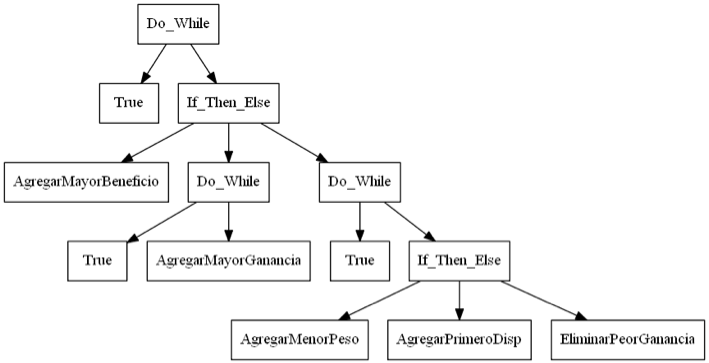
\includegraphics[width=13cm]{images/cap6/AIKPDC2.png}
    \captionof{figure}{Mejor algoritmo del experimento 1 por menor ERP (Elaboración propia, 2015)}\label{fig:AIKPDC2}
\endgroup

%Podría agregar algo respecto a que grupo pertenecen las mejores

Algunas estructuras algorítmicas descubiertas por la PG parecen ser más eficientes que otras en la determinación de la mejor solución para la mochila. Específicamente, es posible apreciar en las figuras que representan los árboles sintácticos que el terminal más utilizado es el de “AgregarMayorGanancia”. Este terminal, en varias ocasiones va acompañado de un ciclo \textit{“while”}, lo que permite llenar la mochila siguiendo el criterio de llenado de este terminal. El terminal que elimina ítems de la mochila que más aparece es “EliminarPeorGanancia”, el cual es utilizado por los algoritmos para eliminar algunos de los elementos y, posteriormente, utilizar otro terminal para llenar el espacio restante. El terminal que aparece posterior al de “EliminarPeorGanancia” es el de “AgregarMenosPeso”, que sirve para agregar un refinamiento al criterio entregado por el terminal de “AgregarMayorGanancia”. Las estructuras siguen la misma lógica de los algoritmos goloso que en algunos casos presenta un refinamiento por medio de la eliminación de algunos ítems para posteriormente realizar un nuevo ingreso de éstos bajo otro criterio.

\subsection{Construcciones inocuas}

Algunos de los algoritmos generados por los métodos utilizados, poseen una estructura inútil o ineficiente. Esto ocurre porque una estructura que deja la mochila vacía, cumple con el criterio de suficiencia, ya que es una posible solución, aunque la calidad de ésta no es buena. Estas soluciones son parte del proceso evolutivo y la forma en que éste las deja de considerar el por medio de la función de evaluación. Algunas de las estructuras generadas son las siguientes:
\begin{itemize}
	\item IfThen(Agregar, Eliminar): esta estructura agrega un elemento y luego lo elimina.
	\item Do\_While(Agregar, Eliminar), Do\_While(True, Eliminar), Do\_While(Eliminar, Eliminar): en estas estructuras ocurre un efecto similar al de la estructura anterior, pero un máximo de tres veces, debido a que el ciclo \textit{“while”} fue implementado con un criterio de término si no genera cambios en la función de evaluación en tres iteraciones.
	\item Not(Eliminar): retorna verdadero, pero no realiza ningún cambio en la mochila.
\end{itemize}

\section{Resultados PVV}

\subsection{Resultados del proceso evolutivo}

Para el problema del vendedor viajero, la GAA converge de forma sistemática para las diversas ejecuciones realizadas. El efecto es similar al ocurrido en el PM-01 y a otros trabajos de la literatura, donde se produce una convergencia en los resultados para ambos experimentos. La Figura \ref{fig:convergencia_exp3} y la Figura \ref{fig:convergencia_exp4} muestran las ejecuciones realizadas por los experimentos 3 y 4 de acuerdo al \textit{fitness} a lo largo de las generaciones. En los gráficos, cada línea corresponde al mejor algoritmo de cada ejecución del programa. En estas figuras es posible apreciar la rápida convergencia de las ejecuciones y que el \textit{fitness} de cada una de éstas converge a un valor similar.

\begingroup
    \centering
    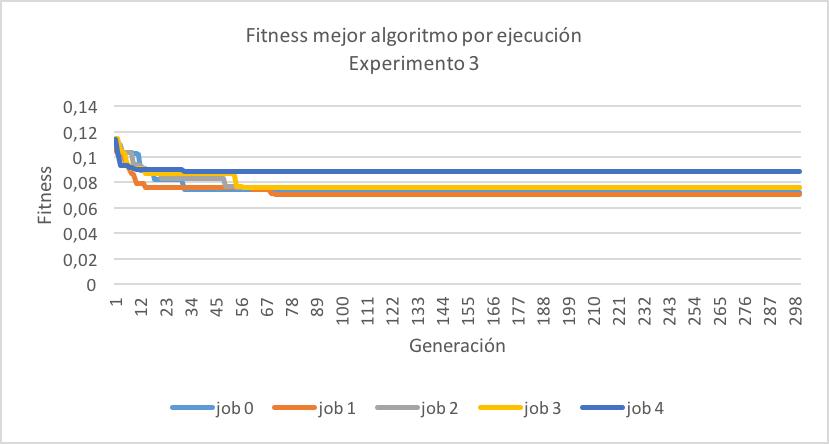
\includegraphics[width=13cm]{images/cap6/convergencia_exp3.png}
    \captionof{figure}{Fitness del mejor algoritmo de cada ejecución por generación para el experimento 3 (Elaboración propia, 2015)}\label{fig:convergencia_exp3}
\endgroup

\begingroup
    \centering
    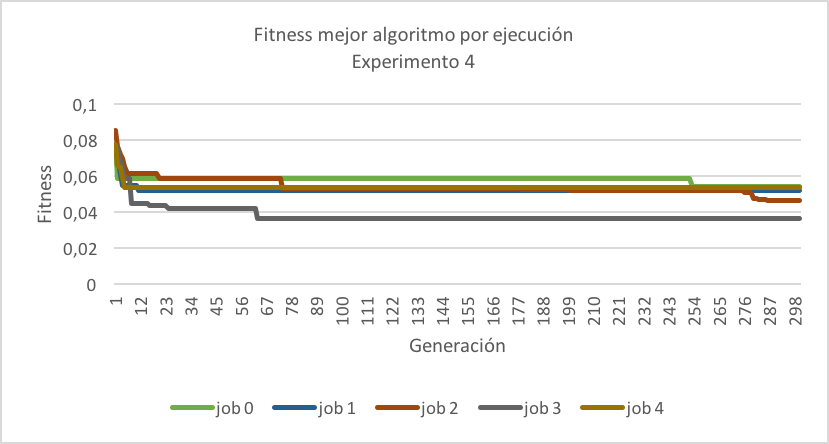
\includegraphics[width=13cm]{images/cap6/convergencia_exp4.png}
    \captionof{figure}{Fitness del mejor algoritmo de cada ejecución por generación ppara el experimento 4 (Elaboración propia, 2015)}\label{fig:convergencia_exp4}
\endgroup

Existe una gran variedad en relación a la calidad de los algoritmos obtenidos. La distribución de los algoritmos por medio de su calidad en el proceso evolutivo a través de las generaciones, es presentada en las Figuras \ref{fig:box_whisker_exp3} y \ref{fig:box_whisker_exp4}. Estas figuras presentan el \textit{fitness} de los algoritmos obtenidos en el proceso evolutivo del experimento 3 y el experimento 4, mediante el uso de un gráfico de \textit{Box and Whisker}. Al igual que para el PM-01, en estas Figuras solo son representadas algunas generaciones (0, 25, 50, 75, …, 299), para así poder apreciar la distribución de los algoritmos, debido a su extensa cantidad de algoritmos generados. Al igual que para el PM-01, es posible inferir que al inicio del proceso evolutivo la mayor cantidad de los individuos posee los peores valores de \textit{fitness}, para el experimento 3 en la generación 0 los cuatro cuartiles se encuentran en un rango de $4.000$ a $4.500$, ya en la generación 25 aparecen individuos con un \textit{fitness} bajo, lo que posiciona los cuartiles en un rango de \textit{fitness} de $0$ a $4.000$ y, posteriormente al avanzar las generaciones se converge a menores valores para la población. Para el experimento 2 se aprecia que en la generación 0 se inicia con un rango de \textit{fitness} de $0$ a $7.000$, donde la mitad de los algoritmos tiene un \textit{fitness} menor a $2.000$, a medida que avanzan las generaciones, esta distribución tiende a mejores valores, los que por la escala generada para mostrar la primera generación no logran apreciarse graficamente, pero éstos oscilan en un rango entre $0$ y $1$, es decir, la “caja” se encuentra dentro del rango mencionado. En general, es posible apreciar que existen varios \textit{outliers} en ambos gráficos, los que se encuentran distribuidos en la parte superior de las “cajas”. En particular el gráfico presentado en la Figura \ref{fig:box_whisker_exp4}, desde la generación 25 en adelante solo es posible apreciar los \textit{outliers}, esto se debe a que las parsimonias aplicadas a este problema empeoran de forma considerable los valores del \textit{fitness}. En ambos gráficos el \textit{fitness} promedio converge a valores menores que oscilan entre $500$ y $1.000$, mientras que la media tiende a $0$ o valores muy pequeños. De esto último, se desprende que los algoritmos tienden a “eliminar” los valores de las parsimonias para mejorar su valor de \textit{fitness} a medida que avanzan las generaciones. La distribución sigue una tendencia de mejora en los resultados de la función de evaluación que es lo esperado. Este efecto ocurre en todas las ejecuciones y aunque la distribución no es igual para todos los casos, sigue una tendencia similar a las presentadas en las figuras descritas anteriormente. La tendencia de los algoritmos puede ser inferida de la Tabla \ref{tab:resumen_exp3} y \ref{tab:resumen_exp4}, donde es posible apreciar que los algoritmos presentan similitudes en sus valores máximos, mínimos y promedio. Dada la cantidad de algoritmos generados, se selecciona para el proceso de evaluación, solo al mejor individuo de cada una de las ejecuciones por experimento. Como resultado, son evaluados 10 algoritmos, siendo cinco los extraídos del experimento 3 y los otros cinco del experimento 4. 

\begingroup
    \centering
    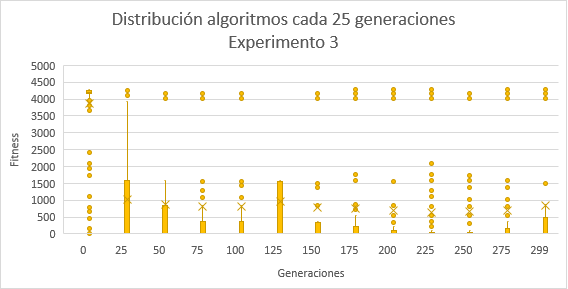
\includegraphics[width=14cm]{images/cap6/box_whisker_exp3.png}
    \captionof{figure}{Distribución de los algoritmos experimento 3 (Elaboración propia, 2015)}\label{fig:box_whisker_exp3}
\endgroup

\begingroup
    \centering
    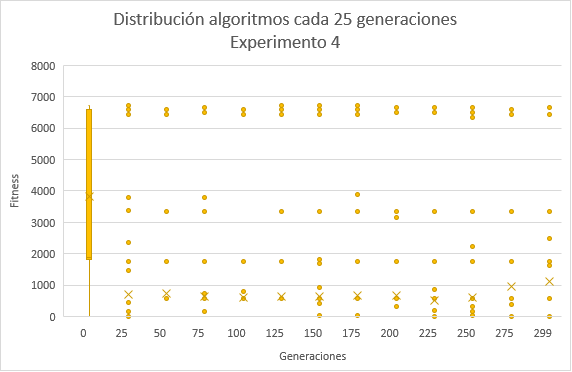
\includegraphics[width=14cm]{images/cap6/box_whisker_exp4.png}
    \captionof{figure}{Distribución de los algoritmos experimento 4 (Elaboración propia, 2015)}\label{fig:box_whisker_exp4}
\endgroup

\begin{table}[ht]
\caption{Datos generales de los algoritmos obtenidos en el experimento 3}\label{tab:resumen_exp3}
\small
\centering
\begin{center}
\rowcolors{2}{gray!25}{white}
\begin{tabular}{c|ccc|ccc|ccc}
\hline
{\textbf{}} & \multicolumn{3}{c}{{\textbf{Fitness}}} & \multicolumn{3}{c}{{\textbf{Nº Nodos}}} & \multicolumn{3}{c}{{\textbf{Altura}}} \\ \hline
{\textbf{Nombre}} & \textbf{Peor} &	\textbf{Prom.} & \textbf{Mejor} & \textbf{Min.} & \textbf{Prom.} & \textbf{Máximo} & \textbf{Min.} & \textbf{Prom.} & \textbf{Máximo} \\ \hline
ejec. 0 & 6731,6667 & 678,8823 & 0,0538 & 2 & 6,4742 & 120 & 2 & 3,1448 & 10 \\
ejec. 1 & 6731,0667 & 1072,3096 & 0,0520 & 2 & 8,7007 & 131 & 2 & 4,1905 & 10 \\
ejec. 2 & 6734,2000 & 867,7404 & 0,0461 & 2 & 9,3059 & 140 & 2 & 4,6702 & 10 \\
ejec. 3 & 6732,2667 & 739,3558 & 0,0364 & 2 & 7,9342 & 126 & 2 & 3,6788 & 10 \\
ejec. 4 & 6733,4000 & 1107,9228 & 0,0533 & 2 & 8,6260 & 133 & 2 & 3,3546 & 9 \\
\hline
\end{tabular}
\end{center}
\caption*{(Elaboración propia, 2015)}
\end{table}

\begin{table}[ht]
\caption{Datos generales de los algoritmos obtenidos en el experimento 4}\label{tab:resumen_exp4}
\small
\centering
\begin{center}
\rowcolors{2}{gray!25}{white}
\begin{tabular}{c|ccc|ccc|ccc}
\hline
{\textbf{}} & \multicolumn{3}{c}{{\textbf{Fitness}}} & \multicolumn{3}{c}{{\textbf{Nº Nodos}}} & \multicolumn{3}{c}{{\textbf{Altura}}} \\ \hline
{\textbf{Nombre}} & \textbf{Peor} &	\textbf{Prom.} & \textbf{Mejor} & \textbf{Min.} & \textbf{Prom.} & \textbf{Máximo} & \textbf{Min.} & \textbf{Prom.} & \textbf{Máximo} \\ \hline
ejec. 0 & 4300,1444 & 849,5119 & 0,0724 & 2 & 11,5701 & 117 & 2 & 5,0646 & 10 \\
ejec. 1 & 4299,8778 & 870,1784 & 0,0708 & 2 & 12,2544 & 104 & 2 & 6,4230 & 10 \\
ejec. 2 & 4303,7444 & 1168,2259 & 0,0758 & 2 & 10,5527 & 146 & 2 & 4,5922 & 10 \\
ejec. 3 & 4301,3444 & 336,8097 & 0,0762 & 2 & 12,6993 & 127 & 2 & 6,0875 & 10 \\
ejec. 4 & 4301,2778 & 1422,5640 & 0,0889 & 2 & 7,0219 & 132 & 2 & 3,4251 & 10 \\
\hline
\end{tabular}
\end{center}
\caption*{(Elaboración propia, 2015)}
\end{table}

No existe una gran variación en la calidad de la GAA para los distintos algoritmos obtenidos durante el proceso evolutivo para el mismo conjunto de instancias. En las tablas \ref{tab:resumen_exp3} y \ref{tab:resumen_exp4} aparecen datos del mejor, peor y promedio del \textit{fitness} de todos los algoritmos generados utilizando alguno de los grupos de instancias clasificados en el sub-capítulo \ref{cap:sel_casos_adapt_pvv}. En relación a la Tabla \ref{tab:resumen_exp3}, es posible apreciar que el resultado tanto del mejor y el peor \textit{fitness} de los algoritmos tiende a valores similares, mientras que el promedio presenta una mayor variación, lo que se debe a la escala de los números obtenidos por la penalización en la función de evaluación (véase \ref{cap:func_eval_pvv}), donde la aparición de uno más o uno menos de los algoritmos con peor \textit{fitness} influye considerablemente. Para la Tabla \ref{tab:resumen_exp4} se ve que ocurre un efecto similar. Finalmente, los resultados que se obtienen en cada uno de los grupos al ser comparados entre experimentos, presentan una variación en la que los algoritmos del experimento 3 obtienen mejores resultados. Esta variación ocurre por que en el experimento 4 se generan algoritmos en distintas poblaciones con distintos criterios de evaluación (islas), lo que conlleva a una mayor variabilidad que la presentada en el experimento 3.

La variación de los algoritmos obtenidos en la GAA está relacionada con la estructura  que posee el árbol sintáctico obtenido durante el proceso evolutivo. Un efecto similar al presentado para los experimentos relacionados al PM-01, ocurre en las tablas \ref{tab:resumen_exp3} y \ref{tab:resumen_exp4}, donde aparecen datos del máximo, mínimo y promedio del número de nodos y la altura. Con respecto al número de nodos, existe variación en los algoritmos que alcanza valores máximos sobre 100, mientras que el promedio es siempre menor a 15, cuyo valor fue determinado como máximo para no interferir en la calidad de los algoritmos (factor de legibilidad, véase \ref{cap:func_eval_pvv}). En relación a la altura de los árboles que representan a los algoritmos, se ve que también existe variación en el promedio. Esto se relaciona directamente con el número de nodos máximo permitido, ya que algunos de estos nodos representan funciones, las que solo tienen permitido un número determinado de hijos.

La calidad de los algoritmos obtenidos mediante el proceso evolutivo no tiene relación con el tiempo que demora el proceso evolutivo ni la generación en la que el o los mejores algoritmos aparecen dentro de la ejecución de este proceso. En las tablas \ref{tab:mejores_pvv_exp3} y \ref{tab:mejores_pvv_exp4}, es posible apreciar el tiempo de evolución de cada una de las ejecuciones y la generación en la que aparece el mejor individuo de ésta. En estas tablas, además, es posible notar que existe variación tanto en el tiempo de cada una de las ejecuciones del proceso evolutivo y en la generación en la que el mejor individuo aparece. El nombre de los algoritmos posee la siguiente forma: Algoritmo - Experimento (Tradicional \textbf{(N)} o co-evolución utilizando método de islas \textbf{(I)}) - Problema - Correlativo de 1 a 5. Un ejemplo de esto último es ANTSP1, que se lee como Algoritmo (A) del experimento tradicional (N) para el problema del vendedor viajero (TSP) obtenido en la ejecución 1.

El tamaño de los árboles que componen los algoritmos obedece al rango de tamaño predefinido en la función de legibilidad que se encuentra dentro de la función de evaluación (\textit{fitness}). En las tablas \ref{tab:mejores_pvv_exp3} y \ref{tab:mejores_pvv_exp4} se muestra que no existe una convergencia hacia árboles de similares dimensiones. Como se observa en estas tablas, los árboles seleccionados varían entre 8 y 15 nodos con una altura entre 4 y 8 para el experimento 3, y entre 3 y 15 nodos, con una altura entre 2 y 6 para el experimento 4.

\begin{table}[ht]
\caption{Datos generales del mejor algoritmo de cada experimento del experimento 3}\label{tab:mejores_pvv_exp3}
\small
\centering
\begin{center}
\rowcolors{2}{gray!25}{white}
\begin{tabular}{cccccc}
{\textbf{{Nombre}}} & {\textbf{{Fitness}}} & {\textbf{\begin{tabular}[c]{@{}c@{}}Nº de \\nodos\end{tabular}}} & {\textbf{{Altura}}} & {\textbf{\begin{tabular}[c]{@{}c@{}}Ejecución en la \\que aparece\end{tabular}}} & {\textbf{\begin{tabular}[c]{@{}c@{}}Tiempo \\(horas)\end{tabular}}}\\ \hline
ANTSP1 & 0,0528 & 13 & 6 & 140 & 24,2040 \\
ANTSP2 & 0,0511 & 15 & 8 & 70 & 23,8845 \\
ANTSP3 & 0,0535 & 15 & 6 & 51 & 19,1857 \\
ANTSP4 & 0,0539 & 15 & 7 & 56 & 24,0360 \\
ANTSP5 & 0,0614 & 8 & 4 & 29 & 14,1123 \\
\hline
\end{tabular}
\end{center}
\caption*{(Elaboración propia, 2015)}
\end{table}


\begin{table}[ht]
\caption{Datos generales del mejor algoritmo de cada experimento del experimento 4}\label{tab:mejores_pvv_exp4}
\small
\centering
\begin{center}
\rowcolors{2}{gray!25}{white}
\begin{tabular}{ccccccc}
{\textbf{{Nombre}}} & {\textbf{{Fitness}}} & {\textbf{\begin{tabular}[c]{@{}c@{}}Nº de \\nodos\end{tabular}}} & {\textbf{{Altura}}} & {\textbf{\begin{tabular}[c]{@{}c@{}}Ejecución en la \\que aparece\end{tabular}}} & {\textbf{\begin{tabular}[c]{@{}c@{}}Isla en la \\que aparece\end{tabular}}} & {\textbf{\begin{tabular}[c]{@{}c@{}}Tiempo \\(horas)\end{tabular}}}\\ \hline
AITSP1 & 0,0803 & 3 & 2 & 2 & 0 & 16,6950 \\
AITSP2 & 0,0558 & 13 & 7 & 271 & 2 & 13,0391 \\
AITSP3 & 0,0621 & 11 & 5 & 182 & 3 & 13,9234 \\
AITSP4 & 0,0544 & 9 & 4 & 62 y 54 & 1 y 3 & 10,8758 \\
AITSP5 & 0,0620 & 15 & 5 & 262 & 2 & 14,9751 \\
\hline
\end{tabular}
\end{center}
\caption*{(Elaboración propia, 2015)}
\end{table}

Las parsimonias utilizadas en los algoritmos no afectan el proceso evolutivo. En los experimentos 3 y 4 se agregaron elementos a la función de evaluación o \textit{fitness} que consideraban una penalización para características propias del problema que generen infactibilidades. Estos elementos empeoran de forma exponencial los valores de la función de evaluación al inicio del proceso evolutivo, y a medida que las generaciones avanzan, estos valores disminuyen llegando a cero. En la Tabla \ref{tab:parsimonias} se puede ver que los elementos de la parsimonia se hacen 0 para todos los mejores algoritmos obtenidos en ambos experimentos. Estos resultados son esperables, ya que las parsimonias afectan en mayor medida (mayor escala) a la función de evaluación, y los elementos que la componen no presentan mayor dificultad, debido a que principalmente se ven afectadas en caso de que los circuitos no estén completos, es decir, se produzca una solución infactible.

\begin{table}[hbtp!]
\caption{Elementos de la parsimonia para los mejores algoritmos de cada experimento.}\label{tab:parsimonias}
\small
\centering
\begin{center}
\begin{tabular}{ccccccc}
{\textbf{Experimento}} & {\textbf{Nombre}} & {\textbf{$ERP$}} & {\textbf{$leg$}} & {\textbf{$PPA$}} & {\textbf{$ERC$}} & {\textbf{$Fitness$}} \\ \hline
Experimento 3		& 	\begin{tabular}[c]{@{}c@{}} ANTSP1 \\ ANTSP2 \\ ANTSP3 \\ ANTSP4 \\ ANTSP5  \end{tabular} &
						\begin{tabular}[c]{@{}c@{}} 0,0528 \\ 0,0511 \\ 0,0535 \\ 0,0539 \\ 0,0614  \end{tabular} &
						\begin{tabular}[c]{@{}c@{}}  0 	   \\ 0 	 \\ 0 	   \\ 0 	 \\ 0 		\end{tabular} &
						\begin{tabular}[c]{@{}c@{}} 4296,6111 \\ 4296,6111 \\ 4296,6111 \\ 4296,6111 \\ 4296,6111 \end{tabular} &
						\begin{tabular}[c]{@{}c@{}}  0 	   \\ 0 	 \\ 0 	   \\ 0 	 \\ 0 		\end{tabular} &
						\begin{tabular}[c]{@{}c@{}} 0,0528 \\ 0,0511 \\ 0,0535 \\ 0,0539 \\ 0,0614  \end{tabular} \\ \hline
Experimento 4		& 	\begin{tabular}[c]{@{}c@{}} AITSP1 \\ AITSP2 \\ AITSP3 \\ AITSP4 \\ AITSP5  \end{tabular} &
						\begin{tabular}[c]{@{}c@{}} 0,0803 \\ 0,0558 \\ 0,0621 \\ 0,0544 \\ 0,0620  \end{tabular} &
						\begin{tabular}[c]{@{}c@{}}  0 	   \\ 0 	 \\ 0 	   \\ 0 	 \\ 0 		\end{tabular} &
						\begin{tabular}[c]{@{}c@{}} 4296,6111 \\ 4296,6111 \\ 4296,6111 \\ 4296,6111 \\ 4296,6111 \end{tabular} &
						\begin{tabular}[c]{@{}c@{}}  0 	   \\ 0 	 \\ 0 	   \\ 0 	 \\ 0 		\end{tabular} &
						\begin{tabular}[c]{@{}c@{}} 0,0803 \\ 0,0558 \\ 0,0621 \\ 0,0544 \\ 0,0620  \end{tabular} \\
\hline
\end{tabular}
\end{center}
\caption*{(Elaboración propia, 2015)}
\end{table}

Los algoritmos generados a partir del proceso evolutivo utilizando el grupo de instancias con un menor coeficiente de correlación obtienen mejores resultados. Para la clasificación de instancias a utilizar por cada una de las islas es utilizado su coeficiente de correlación. En la Tabla \ref{tab:mejores_islas_pvv} se presentan los resultados de los mejores algoritmos de cada isla por ejecución. En esta Tabla se puede ver los resultados del ERP que obtuvo cada uno de éstos y el \textit{fitness} con el que finalmente fueron evaluados durante el proceso evolutivo. Considerando los resultados obtenidos en las ejecuciones de los experimentos donde las islas 0 y 2 utilizan el grupo de instancias 2 y las islas 1 y 3 utilizan el grupo de instancias 1, es posible apreciar que existe una diferencia en la calidad de los resultados de los algoritmos en el proceso evolutivo, que en algunas ejecuciones es menor a un 2\% de ERP al comparar las islas 1 y 3 con las otras islas. Por otra parte, los resultados para las islas 0 y 3, que poseen igual función de evaluación por HITS (cantidad de soluciones óptimas obtenidas), presentan una gran variación entre el ERP y el \textit{fitness}, mientras que en las islas 1 y 2 con función de evaluación por medio de su ERP, obtienen resultados similares. Este efecto es similar al presentado en los resultados del PM-01, donde la función de evaluación, cuando es relacionada a los HITS para obtener el valor del \textit{fitness}, presentan una calidad similar tanto si su ERP es bueno como si no lo es.

\begin{table}[hbtp!]
\caption{Resumen del fitness promedio y ERP de cada isla por ejecución del experimento 4}\label{tab:mejores_islas_pvv}
\small
\centering
\begin{center}
\rowcolors{2}{gray!25}{white}
\begin{tabular}{c|cc|cc|cc|cc}
{\textbf{}} & \multicolumn{2}{c|}{{\textbf{Isla 0}}} & \multicolumn{2}{c|}{{\textbf{Isla 1}}} & \multicolumn{2}{c|}{{\textbf{Isla 2}}} & \multicolumn{2}{c}{{\textbf{Isla 3}}}\\ \hline
{\textbf{Nombre}} & {\textbf{ERP}} & {\textbf{Fitness}} & {\textbf{ERP}} & {\textbf{Fitness}} & {\textbf{ERP}} & {\textbf{Fitness}} & {\textbf{ERP}} & {\textbf{Fitness}} \\ \hline
ejec. 0 & 0,0876 & 0,6667 & 0,0538 & 0,0538 & 0,0638 & 0,0638 & 0,0687 & 0,4444 \\
ejec. 1 & 0,0768 & 0,6667 & 0,0520 & 0,0520 & 0,0540 & 0,0540 & 0,0548 & 0,4444 \\
ejec. 2 & 0,0586 & 0,4444 & 0,0461 & 0,0461 & 0,0545 & 0,0545 & 0,0523 & 0,3333 \\
ejec. 3 & 0,0686 & 0,5556 & 0,0364 & 0,0364 & 0,0521 & 0,0521 & 0,0364 & 0,2222 \\
ejec. 4 & 0,0876 & 0,6667 & 0,0533 & 0,0533 & 0,0582 & 0,0582 & 0,0636 & 0,4444 \\
\hline
\end{tabular}
\end{center}
\caption*{(Elaboración propia, 2015)}
\end{table}

\subsection{Resultados de la evaluación}

Los algoritmos seleccionados para el proceso de evaluación empeoran al comparar los resultados obtenidos para los grupos de instancias de evolución en comparación a los de evaluación. La Figura \ref{fig:evol_vs_eval_exp3_4} muestra los resultados de la comparación entre los resultados de la evolución y evaluación para los experimentos 3 y 4.

\begingroup
    \centering
    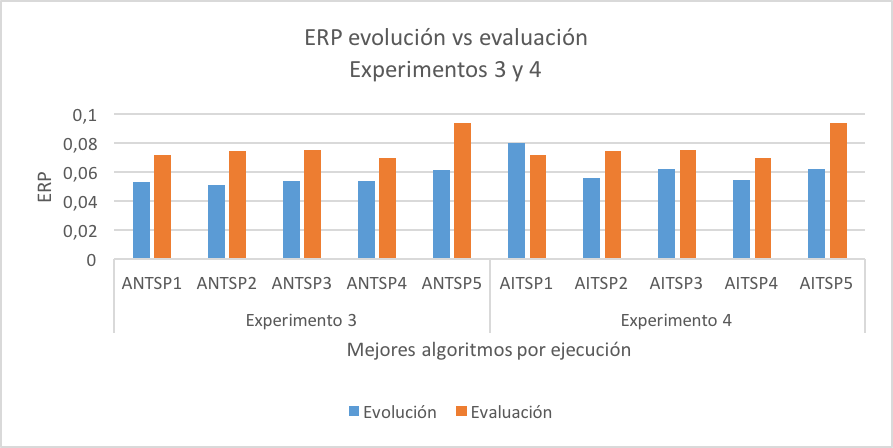
\includegraphics[width=14cm]{images/cap6/evol_vs_eval_exp3_4.png}
    \captionof{figure}{ERP de los resultados obtenidos en la evaluación del grupo de instancias de evolución en comparación al grupo de evaluación (Elaboración propia, 2015)}\label{fig:evol_vs_eval_exp3_4}
\endgroup

Los algoritmos producidos son muy rápidos para resolver los problemas del vendedor viajero. En la Tabla \ref{tab:evol_vs_eval_tiempos_exp3_4} se muestra el tiempo que le toma al mejor algoritmo de cada ejecución resolver las instancias de evaluación para el experimento 3 y 4. El tiempo empleado por los algoritmos del experimento 3 es en promedio 6 minutos y medio, alcanzando menos de 5 minutos el más rápido y casi 11 minutos el más lento de ellos. Los algoritmos más rápidos resuelven en seis segundos aproximados cada instancia, mientras que los más lentos las resuelven en poco más de 12 segundos. Para los algoritmos generados en el experimento 4, se tienen tiempos similares. Estos resultados son esperables, ya que los terminales son acciones con complejidad polinomial y de las funciones sólo el ciclo \textit{while} puede aumentar la complejidad de los algoritmos producidos, sin embargo, este posee una restricción de termino en caso de que en más de tres iteraciones no se produzca algún cambio en el valor de la función de evaluación.
%Agregar el tamaño de las instancias de evaluación.

\begin{table}[hbtp!]
\caption{Tiempo que demoran los mejores algoritmos para resolver las instancias de evaluación}\label{tab:evol_vs_eval_tiempos_exp3_4}
\small
\centering
\begin{center}
\rowcolors{2}{gray!25}{white}
\begin{tabular}{cc|cc}
\multicolumn{2}{c|}{{\textbf{Experimento 3}}} & \multicolumn{2}{c}{{\textbf{Experimento 4}}} \\ \hline
{\textbf{Nombre}} & {\textbf{Tiempo (min)}} & {\textbf{Nombre}} & {\textbf{Tiempo (min)}} \\ \hline
ANTSP1 & 5,7883 & AITSP1 & 5,7883 \\
ANTSP2 & 4,8759 & AITSP2 & 4,8759 \\
ANTSP3 & 5,0715 & AITSP3 & 5,0715 \\
ANTSP4 & 10,5594 & AITSP4 & 10,5594 \\
ANTSP5 & 5,9571 & AITSP5 & 5,9571 \\
\hline
\end{tabular}
\end{center}
\caption*{(Elaboración propia, 2015)}
\end{table}

Los algoritmos obtenidos mediante el proceso co-evolutivo utilizando el método de islas tienen un desempeño computacional similar a los algoritmos obtenidos mediante el proceso tradicional. Los algoritmos obtenidos durante el proceso evolutivo en ambos experimentos para el PVV no logran obtener soluciones óptimas, por lo que no es posible obtener los mejores de acuerdo a la cantidad de soluciones óptimas. Es por esto que sólo se utiliza el criterio de menor ERP para seleccionar a los mejores. En la Tabla \ref{tab:mejores_exp_erp_pvv} se muestran los resultados del mejor algoritmo obtenido para cada experimento de acuerdo a su menor ERP en el grupo de evaluación. En esta Tabla se presentan los indicadores de cada algoritmo y el error relativo que se obtuvo al evaluar los algoritmos con el mismo conjunto de instancias de evaluación y la cantidad de soluciones óptimas que encuentra. 
Tal como se observa, el error relativo promedio de los algoritmos del primer experimento es similar al del segundo experimento. Los resultados obtenidos por ambos experimentos siguen una distribución normal, así lo muestra el \textit{test de Shapiro-Wilk}. En consecuencia,  el \textit{test} de ANOVA que proporciona bajo un 95\% de confiabilidad que no existe diferencia significativa en los datos obtenidos, por lo que no es posible rechazar la hipótesis nula. El resultado contrasta descubrimientos realizados por otros autores para algoritmos genéticos, lo que puede ser inferido puesto que algunos de los resultados obtenidos utilizando el método de la PG con co-evolución muestran una mejora en la calidad de los algoritmos, la que es estadísticamente despreciable.

\begin{table}[hbtp!]
\caption{Mejores individuos por menor ERP en grupo de evaluación}\label{tab:mejores_exp_erp_pvv}
\small
\centering
\begin{center}
\begin{tabular}{cc|ccc|ccc}
\multicolumn{2}{c}{{\textbf{ }}} & \multicolumn{3}{|c|}{{\textbf{Error Relativo}}} & \multicolumn{3}{c}{{\textbf{ }}} \\
{\textbf{Exp.}} & {\textbf{Nombre}} & {\textbf{Peor}} & {\textbf{Prom.}} & {\textbf{Mejor}} & {\textbf{Soluciones}} & {\textbf{Nodos}} & {\textbf{Altura}}\\ \hline
Tradicional & ANTSP4 & 0,1094 & 0,0693 & 0,0114 & 0 & 15 & 7 \\
Islas & AITSP2 & 0,1144 & 0,0672 & 0,0229 & 0 & 13 & 7 \\
\hline
\end{tabular}
\end{center}
\caption*{(Elaboración propia, 2015)}
\end{table}


\subsection{Estructuras de los algoritmos generados}

En esta sección se presenta una figura que muestra el árbol sintáctico del algoritmo junto a una breve explicación de cómo funciona. Los algoritmos descritos en esta sección incluyen los algoritmos señalados en la Tabla \ref{tab:mejores_exp_erp_pvv}. Estos algoritmos son $ANTSP4$ para el experimento 3 y $AITSP2$ para el experimento 4, que fueron seleccionados por obtener el menor ERP al ser evaluados en las instancias de evaluación.

\subsubsection{ANTSP4}

El $ANTSP4$ es el mejor algoritmo obtenido en el experimento 3. En la Figura \ref{fig:ANTSP4} se puede ver el algoritmo por medio de su árbol sintáctico. Este algoritmo posee 15 nodos y una altura de 7, compuesto de 8 terminales y 7 funciones. Este algoritmo sigue una lógica puramente constructiva, donde utilizando distintos criterios tiene por objetivo sólo completar el circuito.

Los pasos a realizar por este algoritmo inician con el ciclo \textit{“while”} con la condición de intentar agregar el mejor vecino. A continuación, pregunta si es posible agregar el mejor vecino y nuevamente aparece la estructura que realiza la misma pregunta. Si ambas son posibles, se intenta agregar una ciudad que genere el menor arco. Posteriormente, si es posible agregar el elemento más cercano al centro, se prosigue a agregar la ciudad que genere el menor arco. Más adelante, se entra a un nuevo ciclo que itera agregando el mejor vecino y la ciudad que genere el menor arco hasta completar el circuito. Finalmente, el circuito creado por el algoritmo es sometido a la heurística \textit{2-opt} para intentar mejorar el resultado.

\begingroup
    \centering
    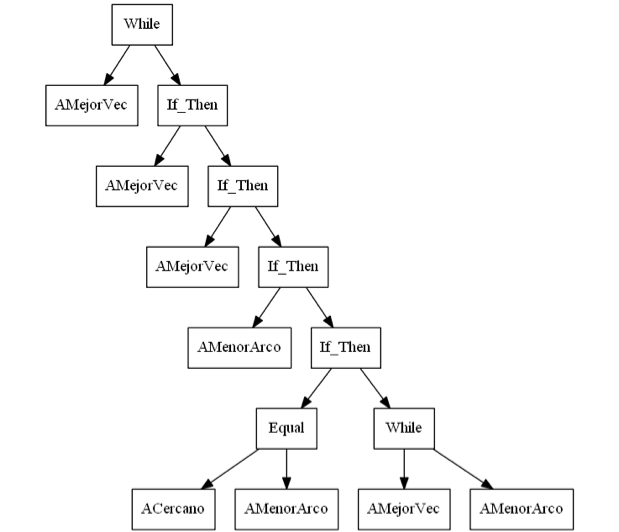
\includegraphics[width=13cm]{images/cap6/ANTSP4.png}
    \captionof{figure}{Mejor algoritmo del experimento 3 (Elaboración propia, 2015)}\label{fig:ANTSP4}
\endgroup

\subsubsection{AITSP2}

El $AITSP2$ es el mejor algoritmo obtenido en el experimento 4. En la Figura \ref{fig:AITSP2} se puede ver el algoritmo por medio de su árbol sintáctico. Este algoritmo posee 13 nodos y una altura de 7, se encuentra compuesto de 6 terminales y 7 funciones. Este algoritmo también sigue una lógica puramente constructiva, donde utilizando distintos criterios tiene por objetivo sólo completar el circuito.
La estructura de este árbol es similar a la obtenida por el mejor algoritmo del experimento 3. En esta estructura se inicia con la adición al circuito del elemento más cercano al centro, para luego agregar la ciudad que genere el menor arco. A continuación, se inicia un ciclo donde si es posible agregar la ciudad que genere el menor arco, se procede a agregar el más cercano al centro. Si esto es posible, se itera agregando la ciudad que genere el menor arco y el mejor vecino hasta completar el circuito. Finalmente, el circuito creado por el algoritmo es sometido a la heurística \textit{2-opt} para intentar mejorar el resultado.

\begingroup
    \centering
    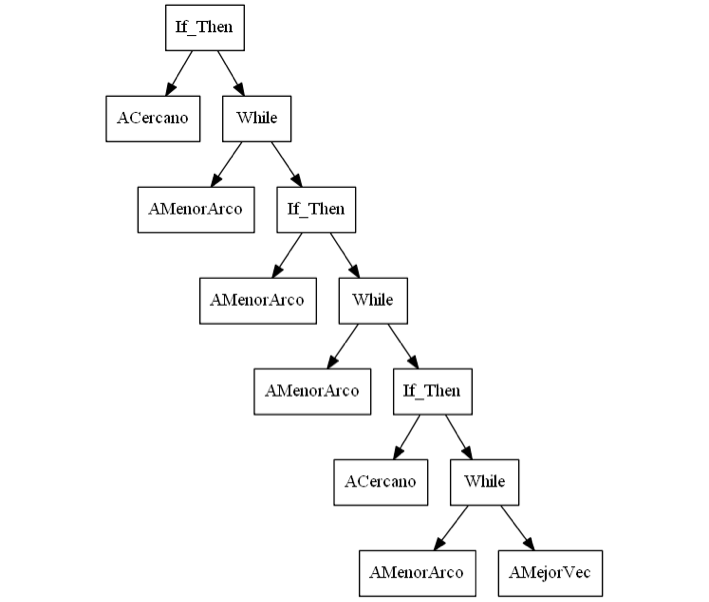
\includegraphics[width=14cm]{images/cap6/AITSP2.png}
    \captionof{figure}{Mejor algoritmo del experimento 4 (Elaboración propia, 2015)}\label{fig:AITSP2}
\endgroup

Algunas estructuras algorítmicas descubiertas por la PG parecen ser más eficientes que otras en la determinación de la mejor solución para el PVV. Específicamente, es posible apreciar en las figuras que representan los árboles sintácticos que los terminales más utilizados son los de “AMenorArco” y “AMejorVecino”. Éstos permiten armar el circuito agregando las ciudades que aumenten en menor medida el costo del circuito con dos criterios. Los criterios son agregar el de menor costo al final y el de agregar una ciudad en cualquier parte del circuito que aumente de menor medida el costo, para “AMenorArco” y “AMejorVecino” respectivamente. El otro terminal que aparece es el de “ACercano”, que agrega al final del circuito la ciudad más cercana al centro. Finalmente, se opera la heurística de optimización \textit{2-opt}, lo que finalmente produce una mejora sustancial sobre las soluciones. En conclusión, los algoritmos generados buscan la producción de un buen circuito para ser optimizado por la heurística \textit{2-opt}.

\subsection{Construcciones inocuas}

Los algoritmos producidos por los experimentos 3 y 4 tienen un efecto similar en algunos de los árboles producidos en los otros experimentos. Algunos de estos efectos son los producidos por las estructuras inútiles. Estas estructuras operan sobre las ciudades del circuito, pero finalmente el resultado es un circuito vacío. Estas soluciones son parte del proceso evolutivo y la forma en que éste las deja de considerar el por medio de la función de evaluación. Algunas de las estructuras generadas son las siguientes:

\begin{itemize}
	\item IfThen(Agregar, Eliminar): esta estructura agrega una ciudad y luego la elimina.
	\item Do\_While(Agregar, Eliminar), Do\_While(True, Eliminar), Do\_While(Eliminar, Eliminar): en estas estructuras se agregan y eliminan elementos de forma iterativa, resultando en que la salida es el circuito vacío.
	\item Not(Eliminar): retorna verdadero, pero no realiza ningún cambio en el circuito.
	\item Las estructuras son similares, ya que los terminales de forma general agregan o eliminan elementos a la solución.
\end{itemize}


\chapter{DISCUSIÓN DE LOS RESULTADOS}
\label{cap:discusion_resultados}

%DESCOMENTAR ESTAS LÍNEAS SI EL CAPÍTULO TIENE FIGURAS O TABLAS
% \addtocontents{lof}{{\bf \noindent Figuras del capítulo \arabic{chapter}}}
% \addtocontents{lot}{{\bf \noindent Tablas del capítulo \arabic{chapter}}}

Durante el proceso evolutivo fueron generados cientos de miles de algoritmos por cada experimento. De estos algoritmos, se escogieron solo los 5 mejores por cada experimento siendo analizados en total 70 de ellos (60 para el PM-01 y 10 para el PVV). A partir de estos algoritmos seleccionados y analizados, se procedió a encontrar a los mejores de cada experimento para realizar un análisis de la estructura de éstos. Los mejores de cada experimento fueron seleccionados en base a dos criterios: el algoritmo que tuviese el menor ERP y el algoritmo que entregase la mayor cantidad de soluciones óptimas. Esto último no se consiguió en el problema del vendedor viajero, ya que ninguno de los algoritmos encontrados pudo obtener soluciones óptimas de las instancias seleccionadas. Por lo que finalmente, para los experimentos 1 y 2 fueron seleccionados los cuatro mejores algoritmos (dos por menor ERP y dos por mayor cantidad de soluciones óptimas) y para los experimentos 3 y 4 los dos mejores de acuerdo al menor ERP obtenido.

Las estructuras encontradas dentro de los mejores algoritmos poseen características similares, por lo que es posible considerar que éstas fueron las más exitosas dentro de la evolución. Para el problema de la mochila bidimensional, la estructura con mayor éxito fue la que contenía los terminales “AgregarMayorGanancia”, “AgregarMenosPeso” y “EliminarPeorGanancia”, donde éstos operan para realizar el llenado de la mochila por medio del terminal “AgregarMayorGanancia”, la que agrega ítems a la mochila de acuerdo a la mayor ganancia (relación $beneficio/peso$), realizando un refinamiento con “EliminarPeorGanancia” que es el inverso del anterior, donde se elimina el de peor ganancia y, posteriormente, utilizar el terminal que agrega los elementos con menor peso “AgregarMenosPeso”. Estos terminales son iterados mediante el uso de las funciones, dentro de las que destacan “Do\_While” e “IfThen”. Los resultados obtenidos por estos algoritmos no superan el $1\%$ de error para los grupos de instancias utilizadas en el conjunto de evaluación en comparación al resultado óptimo de la literatura. En relación a los algoritmos que fueron obtenidos por los experimentos 3 y 4 (para el problema del vendedor viajero), también existen tres terminales que destacan dentro de la estructura “AMenorArco”, “AMejorVecino” y “ACercano”. Estos terminales siguen una estructura que busca armar el circuito de forma completa, sin realizar cambios eliminando parte del circuito. La forma en que estos terminales opera se basa, principalmente, en agregar el circuito que genere el arco de menor costo utilizando el terminal “AMenorArco”. Los otros terminales (“AMejorVecino” y “ACercano) operan para obtener un pequeño tramo del circuito, el que da paso para completar el circuito con el terminal “AMenorArco”. Al igual que los algoritmos obtenidos en los experimentos 1 y 2, éstos operan utilizando principalmente las mismas funciones (“Do\_While” e “IfThen”). Los resultados obtenidos por los algoritmos para el PVV promedian el $7\%$ de error para los grupos de instancias utilizadas en el conjunto de evaluación en comparación al resultado óptimo de la literatura.

Los mejores algoritmos generados por los métodos utilizados poseen un tamaño (cantidad de nodos) reducido, siendo los más grandes de 15 nodos. Este tamaño fue el determinado como número máximo de nodos permitido y todos los mejores algoritmos tienden a lo más, a este tamaño. El tamaño permite realizar un análisis sobre la estructura que éstos poseen con el fin de identificar el funcionamiento y sus principales características. Este análisis de la estructura permite identificar a los algoritmos como heurísticas constructivas y con algún tipo de refinamiento (en el caso de los relacionados al PM-01) y solo constructivas (para los relacionados al PVV).

La sobre-especialización de los algoritmos obtenidos mediante ambos métodos pudo ser constatada para los algoritmos obtenidos por los experimentos 1 y 2 (PM-01). Dada la gran cantidad de instancias y las clasificaciones realizadas para éstas en la literatura \citep{pisinger_2005}, se pudo realizar gran variedad de sub-experimentos, los que permitieron dar a conocer para el conjunto de terminales y funciones definidos, las instancias más fáciles y más difíciles de resolver; además, los algoritmos tienden a sobre-especializarse cuando todas las instancias utilizadas en el proceso evolutivo poseen las mismas características. Otro factor que pudo ser constatado gracias a la clasificación de instancias, fue que los algoritmos durante el proceso evolutivo obtienen mejores resultados para instancias de mayor tamaño.

Para los experimentos 2 y 4 se utilizaron diferentes funciones de evaluación (por HIT y por ERP). Al analizar la calidad que tienen los algoritmos generados en base a su ERP en comparación a su función de evaluación, fue posible determinar que en los casos donde se utiliza la función de evaluación por HIT, para algunos casos el ERP era menor que el obtenido por las que utilizan la función de evaluación con ERP. Esto se debe a que los algoritmos evaluados con la función por HIT, deben cumplir con un error relativo máximo para que sea considerado, resultando en que a pesar de que el ERP sea bajo, el valor de su función de evaluación no lo es. Por otra parte, esta evaluación por HIT califica de igual manera a un algoritmo que no alcanza un mejor valor que el máximo permitido.

Las parsimonias aplicadas durante el proceso evolutivo para los experimentos relacionados al PVV no afectan los resultados. Las parsimonias utilizadas en estos experimentos fueron para forzar o dirigir los algoritmos de acuerdo al conocimiento del problema para obtener soluciones factibles de éstos y para que el tamaño de los algoritmos no supere un número determinado. En todos los resultados obtenidos por los mejores algoritmos, las parsimonias tienen valor 0, esto permite dar pie a considerar incluir otras que posean características del problema.

La relación entre los experimentos por cada problema (1 con 2 y 3 con 4), no logra obtener una diferencia significativa en la calidad de los resultados, por lo que no es posible determinar que las muestras sean estadísticamente diferentes. Es decir, no es posible determinar que un método sea mejor que el otro. Sin embargo, una de las diferencias se encuentra en el tiempo que le toma al proceso evolutivo llevar a cabo cada una de las ejecuciones, donde el tiempo más significativo puede ser encontrado en los relacionados al PVV, éstos promedian 21 horas para el experimento 3 y 16 horas para el experimento 4. Con estos resultados surgen algunas preguntas que pueden ser planteadas para la PG utilizando co-evolución con islas que ameritarían una nueva experimentación, tales como: ¿cuál es el número óptimo de islas?, ¿cuál es el tamaño óptimo de la población global?, ¿deberían las islas tener la misma población?, ¿las funciones de evaluación utilizadas permiten seleccionar siempre a los mejores individuos o deben ser modificadas?, ¿es conveniente utilizar el método con co-evolución por la diferencia en el tiempo empleado en el proceso evolutivo?. Adicionalmente, al producir algoritmos que se generan de forma automática y presentan novedad, se abre la posibilidad de mejorar los elementos con el que fueron diseñados los experimentos, de esta forma surgen otras preguntas como: ¿el tamaño de las instancias utilizadas en el proceso evolutivo debe ser mayor?, ¿son el conjunto de funciones y terminales adecuados para resolver los problemas?, ¿existen elementos que considerar como parsimonia dentro de la función de evaluación?.


\chapter{CONCLUSIONES}
\label{cap:conclusiones}

%DESCOMENTAR ESTAS LÍNEAS SI EL CAPÍTULO TIENE FIGURAS O TABLAS
% \addtocontents{lof}{{\bf \noindent Figuras del capítulo \arabic{chapter}}}
% \addtocontents{lot}{{\bf \noindent Tablas del capítulo \arabic{chapter}}}

El desarrollo de este trabajo tenía como objetivo general comparar los algoritmos obtenidos mediante el uso de los métodos de PG tradicional con el de PG con co-evolución para los problemas de la mochila binaria y el problema del vendedor viajero.

En base al estudio del estado del arte y revisión de la literatura, se ha podido encontrar que existen diversas técnicas para afrontar estos problemas con buenos resultados. Sin embargo, aun queda trabajo por realizar, ya que mientras no se encuentre la solución para éstos problemas, los estudios sobre estos siguen sumando importancia. Dentro de estos estudios, la PG como una hiper-heurística sigue cobrando mayor importancia.

Los resultados de este estudio indican que los algoritmos tienen alta eficiencia y efectividad para resolver los problemas. Específicamente, los algoritmos para el PM-01 obtienen resultados que son similares al óptimo, en promedio $0,1\%$ de error que son similares a los obtenidos por otros autores utilizando la PG \citep{sepulveda_2011, parada_2015} y los del PVV un $7\%$ de error que igualmente poseen similitud a los obtenidos en la literatura \citep{sepulveda_2011}. Estos resultados pueden ser constatados en la tabla de resultados, donde cada algoritmo fue evaluado con un conjunto de instancias de evaluación las que contenían tanto similares como diferentes características a las utilizadas en los casos de adaptación del proceso evolutivo.

No todos los terminales ni funciones aparecen en las estructuras de los algoritmos obtenidos, lo que indica claramente que algunas de éstas son mejores durante el proceso evolutivo. Como se especificó en los capítulos donde se habla de las estructuras y en los resultados, sólo algunos de los terminales y funciones destacan para cada problema, siendo muchos más los utilizados. Para el PM-01, ocurre un proceso de llenado y refinamiento de la mochila, mientras que para el PVV se arma el circuito de menor costo para posteriormente refinarlo utilizando la heurística \textit{2-opt}.

Las instancias obtenidas para el desarrollo del experimento, han servido para concluir respecto a la importancia que tienen las características propias de éstas para la GAA, de acuerdo a su clasificación para la calidad de los los resultados que finalmente obtienen los algoritmos. En particular destacan las clasificaciones utilizadas en los experimentos 1 y 2, las que permiten concluir que la sobre-especialización con la que se generan los algoritmos para determinados grupos. Además, permiten dar a conocer que instancias que generan los mejores algoritmos en el proceso evolutivo, son las que presentan mayor diversidad entre beneficio y peso, mientras que las peores tienen una relación directa o de igualdad. Por otra parte, la clasificación de instancias para el PVV, los resultados del proceso evolutivo y los hallazgos sobre la sobre-especialización en el PM-01, permiten inferir que un grupo de instancias con un menor coeficiente de correlación son mejores para la calidad de los algoritmos generados.

La PG es un proceso en el que se explora combinaciones de diversos componentes elementales de heurísticas, que entregan un resultado de acuerdo a alguna combinación de estos componentes. Al incluir el método de co-evolución, resultó solo en una nueva forma de explorar de estas combinaciones alcanzando valores muy similares a los obtenidos por la PG tradicional. Finalmente, no es posible mostrar una diferencia estadística sobre los resultados obtenidos mediante el uso de PG con co-evolución en comparación a los obtenidos utilizando la PG de forma tradicional, por lo que las Hipótesis presentadas en este trabajo son rechazadas.



% ----------------------------------------------------------
% ----------- TERCERA PARTE --------------------------------
% \backmatter %Elimina la numeraci�n
% ### Bibliograf�a de este documento ###
\bibliographystyle{apa-good}
\bibliography{referencias}

% ----------------------------------------------------------
% ----------- CUARTA PARTE ---------------------------------
%\appendix
%\addappheadtotoc %agregar ap�ndice al i�ndice. Si no tiene ap�ndices COMENTAR o BORRAR
% \noappendicestocpagenum %quitar n�mero de p�ginas a los ap�ndices
% ### APENDICES ###
%\fontsize{9}{10.8} %tama�o de letra para ap�ndices es 9pt
%\linespread{1.0} %interlineado de 1 para los ap�ndices
%\small % Lo mismo que lo anterior, haber si funciona

%\include{apendices/Apendice-1} % Manuales de Usuario
%\include{apendices/Apendice-2} % Eventos
%\include{apendices/Apendice-3} % Clases
%\include{apendices/Apendice-4} % Peticiones HTTP y objetos transferidos
%\include{apendices/Apendice-5} % Uso de memoria
%\include{apendices/Apendice-6} % Archivos de entrada
%\include{apendices/Apendice-7} % C�digo fuente de ejemplo de aplicaci�n concreta
\end{document} %\\end
